\chapter{Анализ потоков тепла на основе динамико-стохастической модели}
\label{chc:Analysis}
Рассмотрим результаты, полученные с использованием описанных в главе~\ref{ch:Methods} методов к данным реанализа из базы ERA5 по акватории Северной Атлантики. 


В данной главе рассматривается взаимное влияние этих величин, выявляются области преобладания диффузионной составляющей над дрейфовой. Поскольку параметр диффузии является матричной величиной, эта матрица векторизована с использованием разложения на собственные векторы и значения. Физический смысл этих разложений и результирующие пространственные структуры, а также их изменения во времени соответствуют системе океанских течений в атлантической меридиональной опрокидывающей циркуляции~\cite{Caesar2018} и крупномасштабным тепловым волнам.

Рассматриваются как точечные оценки случайных коэффициентов $a(t,X)$ и $b(t, X)$ в СДУ Ито~\eqref{eq:Ito}, так и взаимосвязи между ними за почти $44$ года наблюдений. Расчеты проведны для различных осреднений (сутки, месяц и т.д.), результаты отображаются на динамических картах для рассматриваемого временного интервала для всех изучаемых точек акватории Северной Атлантики. Ниже приведены примеры построенных карт для некоторых выбранных моментов времени, демонстрирующие описываемые эффекты.


\section{Данные реанализа}
В работе изучаются данные реанализа базы ERA5 явного и скрытого потоков тепла, температуры поверхности океана (Sea Surface Temperature -- SST) и атмосферного давления в Северной Атлантике за период с $1$ января $1979$ года по $31$ декабря $2024$ года.
Данные сосредоточены в узлах равномерной сетки с шагом в $0.5$ градуса, покрывающей область Северной Атлантики. Границы сетки по широте составляют от $-90$ до $0$ градусов, а по долготе -- от $0$ до $80$ градусов. Шаг измерений по времени составляет $6$ часов, на одни сутки приходится $4$ измерения: в полночь, $06:00$, $12:00$ и $18:00$.

На рисунке~\ref{fig:flux_example} представлен пример визуализации данных потоков тепла с суточным усреднением: график слева соответствует явным, а справа -- скрытым потокам тепла. Цветовая шкала меняется от синего (при отрицательных значениях потоков) до белого (при значениях, близких к нулю) и далее до красного (при положительных значениях). Яркость цвета в конкретной точке соответствует удаленности значения от нуля. Темно-зеленым цветом обозначены участки суши.

\begin{figure}[!h]
	\centering
	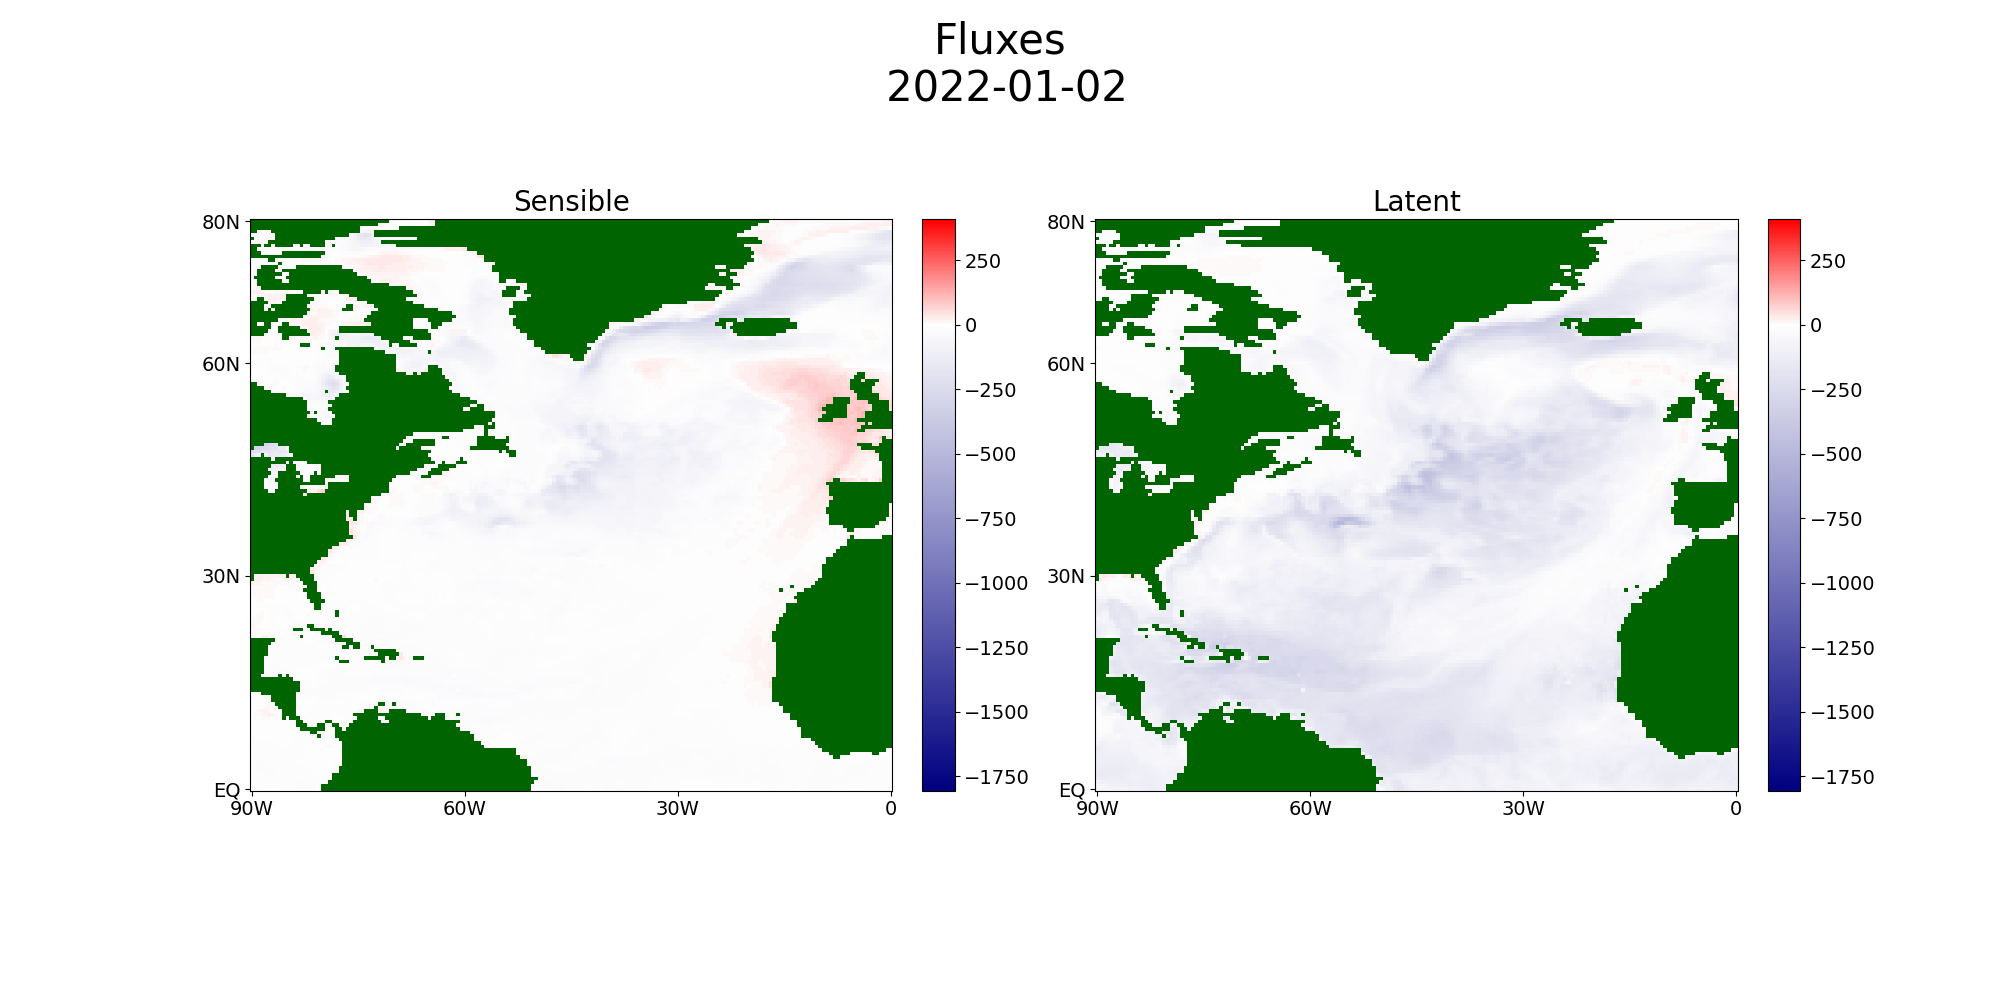
\includegraphics[width=\textwidth]{Flux_00002}
	\caption{Пример визуализация данных по акватории Северной Атлантики с суточным усреднением: слева -- явные, справа -- скрытые потоки}
	\label{fig:flux_example}
\end{figure}


На рисунке~\ref{fig:data_example} показан пример визуализации данных суммарного потока тепла, SST и давления с ежедневным усреднением: картинка слева соответствует суммарному тепловому потоку, в середине - температуре поверхности океана, а справа -- атмосферному давлению. Цветовая шкала на левом графике меняется с синего (при отрицательных значениях) до белого (при значениях, близких к нулю), а затем до красного (при положительных значениях). Яркость цвета в определенной точке соответствует удаленности модуля значения от нуля. Для среднего и правого графиков, очевидно, значения могут быть только положительными, поэтому их шкала значений варьируется от белого (при значениях, близких к нулю) до ярко-красного. Светло-зеленый цвет обозначает участки суши.


\begin{figure}
	\centering
	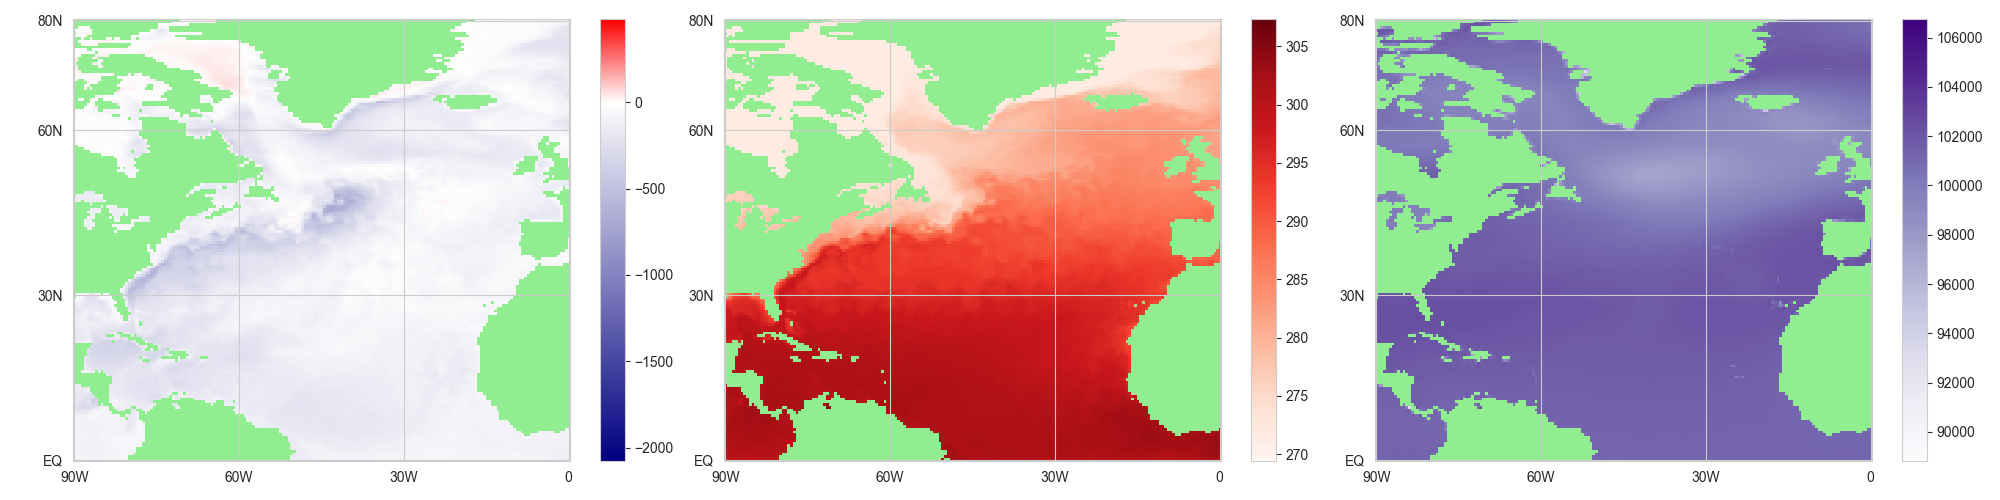
\includegraphics[width=\textwidth]{16436.png}
	\caption{Пример используемых данных: суммарный тепловой поток, SST и атмосферное давление, усредненные данные за $1$ января $2024$ года}
	\label{fig:data_example}
\end{figure}

Три рассмотренные переменные сильно коррелируют друг с другом, что видно из их попарных корреляций. Пример корреляций за $7$ дней показан на рисунке~\ref{fig:correlations}. В то же время нельзя говорить о существовании какого-то одного типа зависимости: скорее, выделяются определенные области или зоны с положительными или отрицательными корреляциями.

\begin{figure}
	\centering
	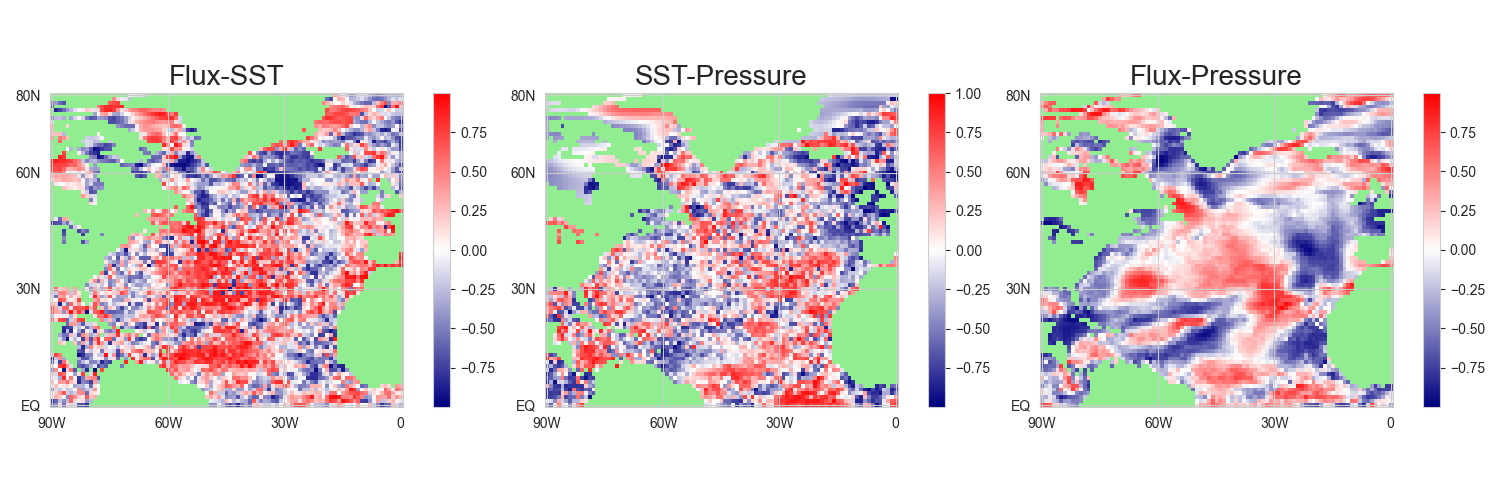
\includegraphics[width=\textwidth]{Correlations.png}
	\caption{Попарные корреляции суммарного теплового потока, SST и атмосферного давления за период $01.01.2024-08.01.2024$}
	\label{fig:correlations}
\end{figure}

%Теперь оба метода применяются к данным пространственно-временного реанализа тепловых потоков между океаном и атмосферой в Северной Атлантике за период $1979-2022$ годов. Для проверки и сравнения результатов методов на реальных данных используются данные повторного анализа из базы данных ERA5 для явных и скрытых тепловых потоков, описанные в разделе \ref{Data}.

\section{Проверка существования решения СДУ на используемых данных}
\label{app:Existance}
Решением СДУ вида~\eqref{eq:Ito} является диффузионный процесс с коэффициентом диффузии $b^2(t,X)$ и коэффициентом переноса $a(t,X)$. Случайные коэффициенты $a(t,X)$ и $b(t,X)$ представляют собой условное математическое ожидание и дисперсию приращений потока соответственно:
\begin{gather*}
	a(t,X) = \frac{\E(X(t+dt)-X(t)|X(t)=x)}{dt}, \quad
	% 		\end{equation}
% 		\begin{equation}
	b(t,X) = \frac{\D(X(t+dt)-X(t)|X(t)=x)}{dt}.
\end{gather*}

Предположим, что $a(t,X)$ и $b(t,X)$ –- борелевские функции, определенные при $x \in \R^1$, $t \in [t_0,T]$. Тогда рассматриваемое СДУ эквивалентно следующему уравнению (начальное условие $X(t_0)$ предполагается заданным):
\begin{equation}
	\label{integral_Ito}
	X(t) = X(t_0) + \int_{t_0}^{t} a(s, X(s))ds + \int_{t_0}^{t} b(s, X(s))dW(s).
\end{equation}

Для существования решения уравнения~\eqref{integral_Ito} для некоторого $K$ необходимо~\cite{Skorohod} выполнение условий вида:
\begin{enumerate}
	\item для всех $x$ и $y \in \R^1$: 
	% 			\begin{equation*}
		$|a(t,x)-a(t,y)|+|b(t,x)-b(t,y)| \leqslant K|x-y|$,
		% 			\end{equation*}
	\item для всех $x \in \R^1$: 
	% 			\begin{equation*}\
		$|a(t,x)|^2+|b(t,x)|^2 \leqslant K(1+x^2)$.
		% 			\end{equation*}
\end{enumerate}

Причем если при этом $X_1 (t)$ и $X_2(t)$ -– два непрерывных решения уравнения \ref{integral_Ito}, то они неразличимы.
% 		\begin{equation*}
	% 			\P \left\lbrace \sup_{t_0 \leqslant t \leqslant T} |X_1(t) - X_2(t)| > 0 \right\rbrace = 0.
	% 		\end{equation*}
% 		Более того, при условиях этой теоремы решение уравнения~\ref{integral_Ito} будет процессом Маркова, вероятности перехода которого определяются соотношением:
% 		\begin{equation*}
	% 			P(t,x,s,A)= P\left\lbrace X_(t,x) (s) \in A\right\rbrace 
	% 		\end{equation*}

Проверим выполнение этих условий для анализируемых данных, а именно -- найдем оценку константы $K$. Для неравенства из первого пункта естественным образом будем рассматривать случай $x \ne y$. Имеем:
% 		Оценим константу $K$ в этом неравенстве отдельно для каждого потока следующим образом: найдем минимум выражения $|x-y|$ при $x \ne y$ для всех значений потоков $x$ и $y$, имеющихся в данных. Затем для каждого $t \in [t_0,T]$ максимизируем разности $|a(t,x)-a(t,y)|+|b(t,x)-b(t,y)|$ и возьмем максимум по $t$. Тогда для 
\begin{equation*}
	K \geqslant \frac{\max(|a(t,x)-a(t,y)|+|b(t,x)-b(t,y)|)}{\min(|x-y|)}.
\end{equation*}
% 	первое неравенство будет выполнено для рассматриваемого типа потока. Для того, чтобы получить универсальную константу для обоих типов потоков, возьмем максимум из двух оценок.

Для второго неравенства, учитывая, что $(1+x^2 )\geqslant 1$, получим:
\begin{equation*}
	K \geqslant \max\limits_{x \in \R^1, t \in [t_0,T]}(|a(t,x)|^2 + |b(t,x)|^2).
\end{equation*}
% 	где максимум берется по всем присутствующих в данных значениям потока $x$ и при всех $t \in [t_0,T]$.

В данных присутствует небольшое количество выбросов, которые могут в несколько раз превосходить типичные значения коэффициентов. Для определения коэффцициентов в неравенствах они могут быть исключены: в качестве максимума для каждого типа потока выбирается квантиль порядка $0.97$, а в качестве минимума – $0.03$. 
В силу объема данных вычисление квантилей на всем промежутке времени одновременно затруднительно, поэтому квантили считались на отрезках по $1000$ дней, а затем в качестве верхней квантили брался максимум из них на каждом отрезке, а в качестве нижней –- минимум. Кроме того, введем условие отделимости от $0$ разности $x-y$, эмпирически выбран порог $0.1$.

С учетом введенных ограничений были получены следующие значения верхних и нижних квантилей для $a$ и $b$: $b_{up} = 148.02$, $b_{low} = 0$ (из физического смысла, случаи комплексных $b$ и потому отрицательных значений не рассматриваются), $a_{up} = 40.77$, $a_{low} = -32.02$. При таких введенных ограничениях получаем оценку на K для первого неравенства	$K_1 \geqslant 2209$ и для второго -- 	$K_2 \geqslant 23572$. 	Таким образом, необходимое конечное значение $K$ существует, гарантируя корректность применяемой в работе математической модели.


\section{Коэффициент сноса}
Рассмотрим сначала оценки для коэффициента сноса $a(t,X)$, то есть динамической составляющей процесса.
При визуализации (см. рисунок~\ref{fig:ab_mean_year}) используется цветовая шкала, аналогичная потокам на рисунке~\ref{fig:flux_example}: цвет меняется от темно-синего при отрицательных значениях полученных оценок до белого при значениях, близких к нулю, и далее до темно-красного при увеличении положительных значений. Яркость цвета в конкретной точке соответствует удаленности значения от нуля. Темно-зеленым цветом обозначены участки суши.

По результатам анализа многолетних данных установлено, что максимумы динамической составляющей соответствуют направлению основного потока Гольфстрима. Типичной для коэффициента сноса является ситуация, в которой в фиксированной точке направление движения потока меняется на противоположное быстрее, чем за сутки. На динамических картах это выражается в изменении ее раскраски с синего цвета на красный (или наоборот) при отрисовке двух подряд идущих дней.

В период с октября по апрель наблюдаются более высокие абсолютные значения оценок (что соответствует более ярким цветам на картах), в то время как в летние месяцы значения носят более умеренный характер. В таблице~\ref{tab:quantiles_a} представлены диапазоны между квантилями уровня $0.1$ и $0.9$ в летний и зимний периоды для полученных оценок коэффициента сноса двух типов потоков - $a_1$ и $a_2$, соответственно. 

\begin{table}[h!]
	\centering
	\caption{Диапазоны значений в летние и зимние периоды между квантилями уровня $0.1$ и $0.9$ для $a_1$ и $a_2$}
	\begin{tabular}{|c|c|c|c|c|}
		\hline
		Период & 1979-1989гг. &  1989-1999гг. & 1999-2009гг. & 2009-2019гг.\\
		\hline
		$a_1$, лето & $[-3.8, 4.1]$ & $[-4.1, 4.1]$ & $[-4.1, 4.3]$ & $[-4.1, 4.3]$\\ 
		\hline
		$a_1$, зима & $[-11.2, 10.2]$ & $[-12.2, 10.5]$ & $[-11.6, 10.9]$ & $[-10.2, 8.9]$\\ 
		\hline
		$a_2$, лето & $[-13.1, 13.8]$ & $[-13.5, 13.8]$ & $[-14.1, 14.8]$ & $[-14.5, 15.5]$\\
		\hline
		$a_2$, зима & $[-23.9, 24.7]$ & $[-24.9, 25.6]$ & $[-24.1, 26.2]$ & $[-24.6, 25.4]$\\ 
		\hline
	\end{tabular}
	\label{tab:quantiles_a}
\end{table}

Для наглядной демонстрации этого эффекта на рисунке~\ref{fig:ab_mean_year} изображены оценки коэффициента сноса по акватории за так называемый средний год: для $6$ выбранных дней за год в различные сезоны ($15$ февраля, апреля, июня, августа, октября и декабря) для явного (рисунок~\ref{fig:ab_mean_year}a)) и скрытого (рисунок~\ref{fig:ab_mean_year}b)) потоков усредняются наблюдения за $43$ анализируемых года ($1979$--$2021$ гг.). Полные данные за $2022$ год на момент подготовки текста еще не были доступны, поэтому в данном случае в расчетах не использовались.

\begin{figure}[h!]
	\center{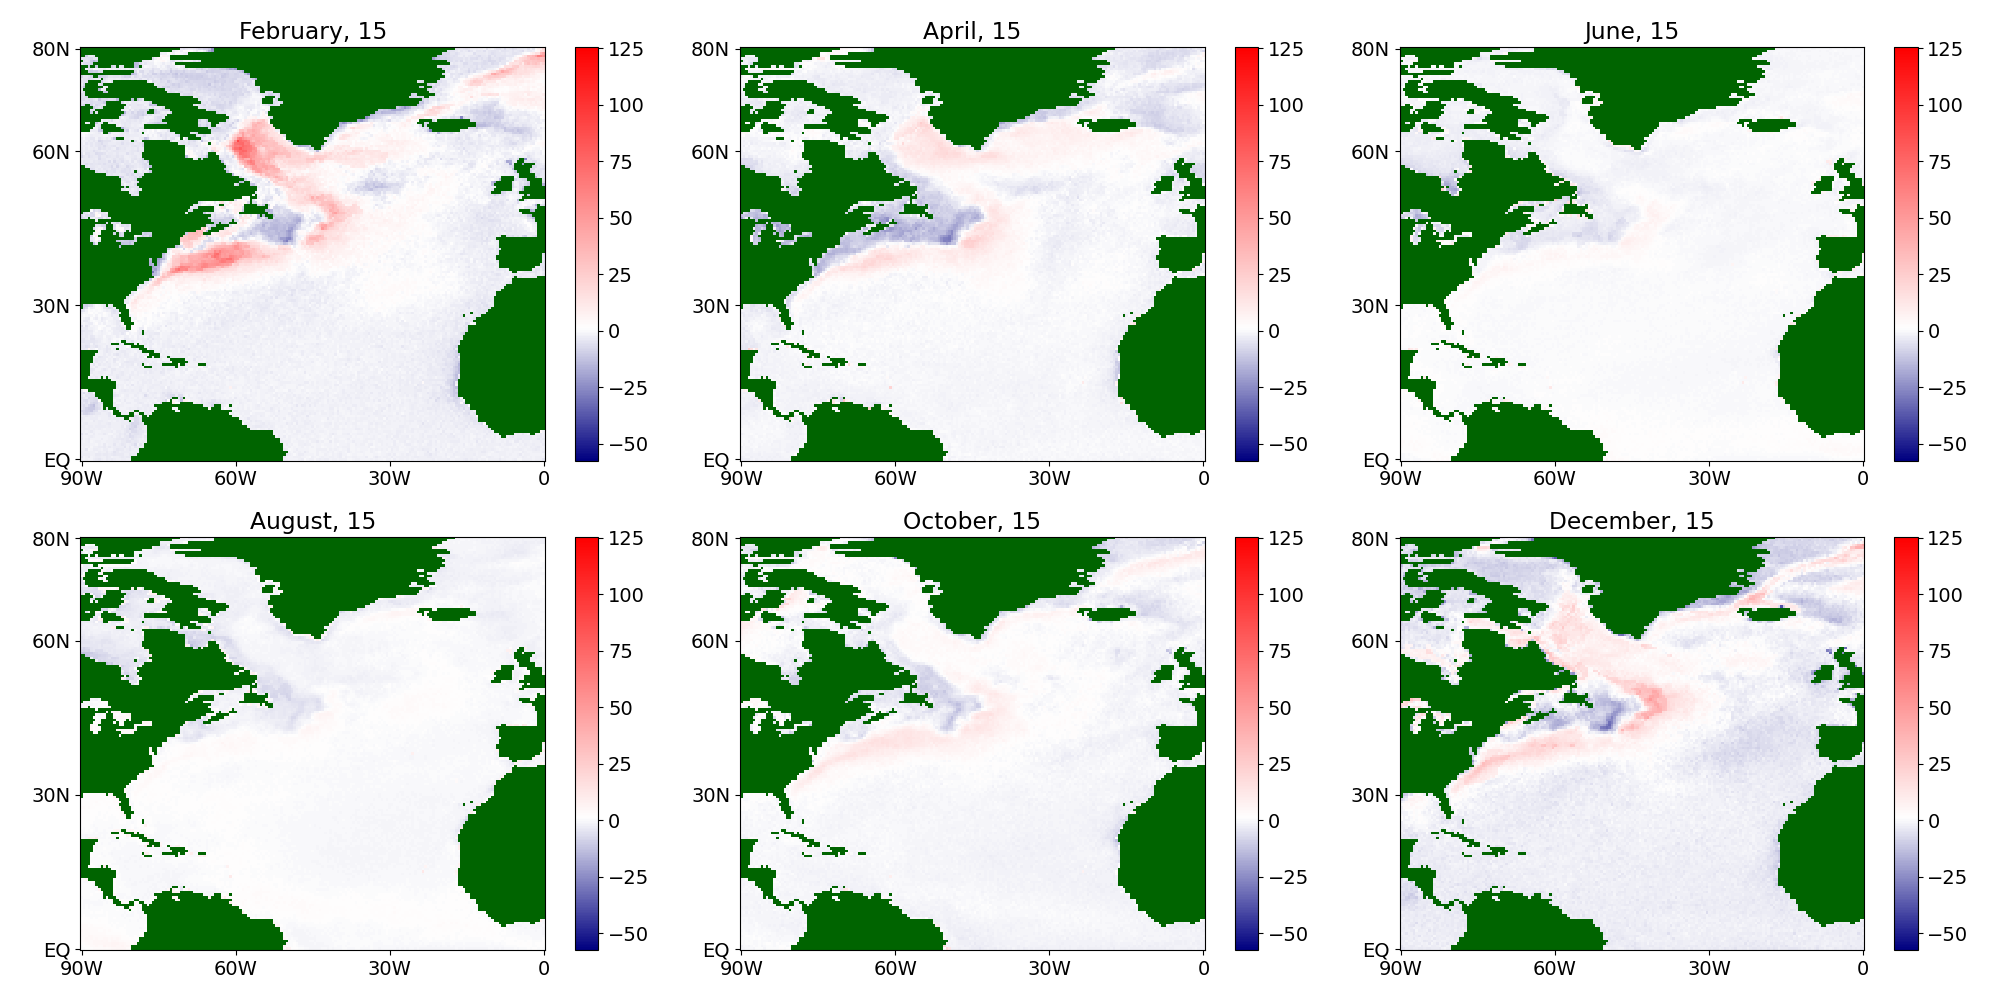
\includegraphics[width=\textwidth]{A_sens_mean_year}}\\
	a)
	\center{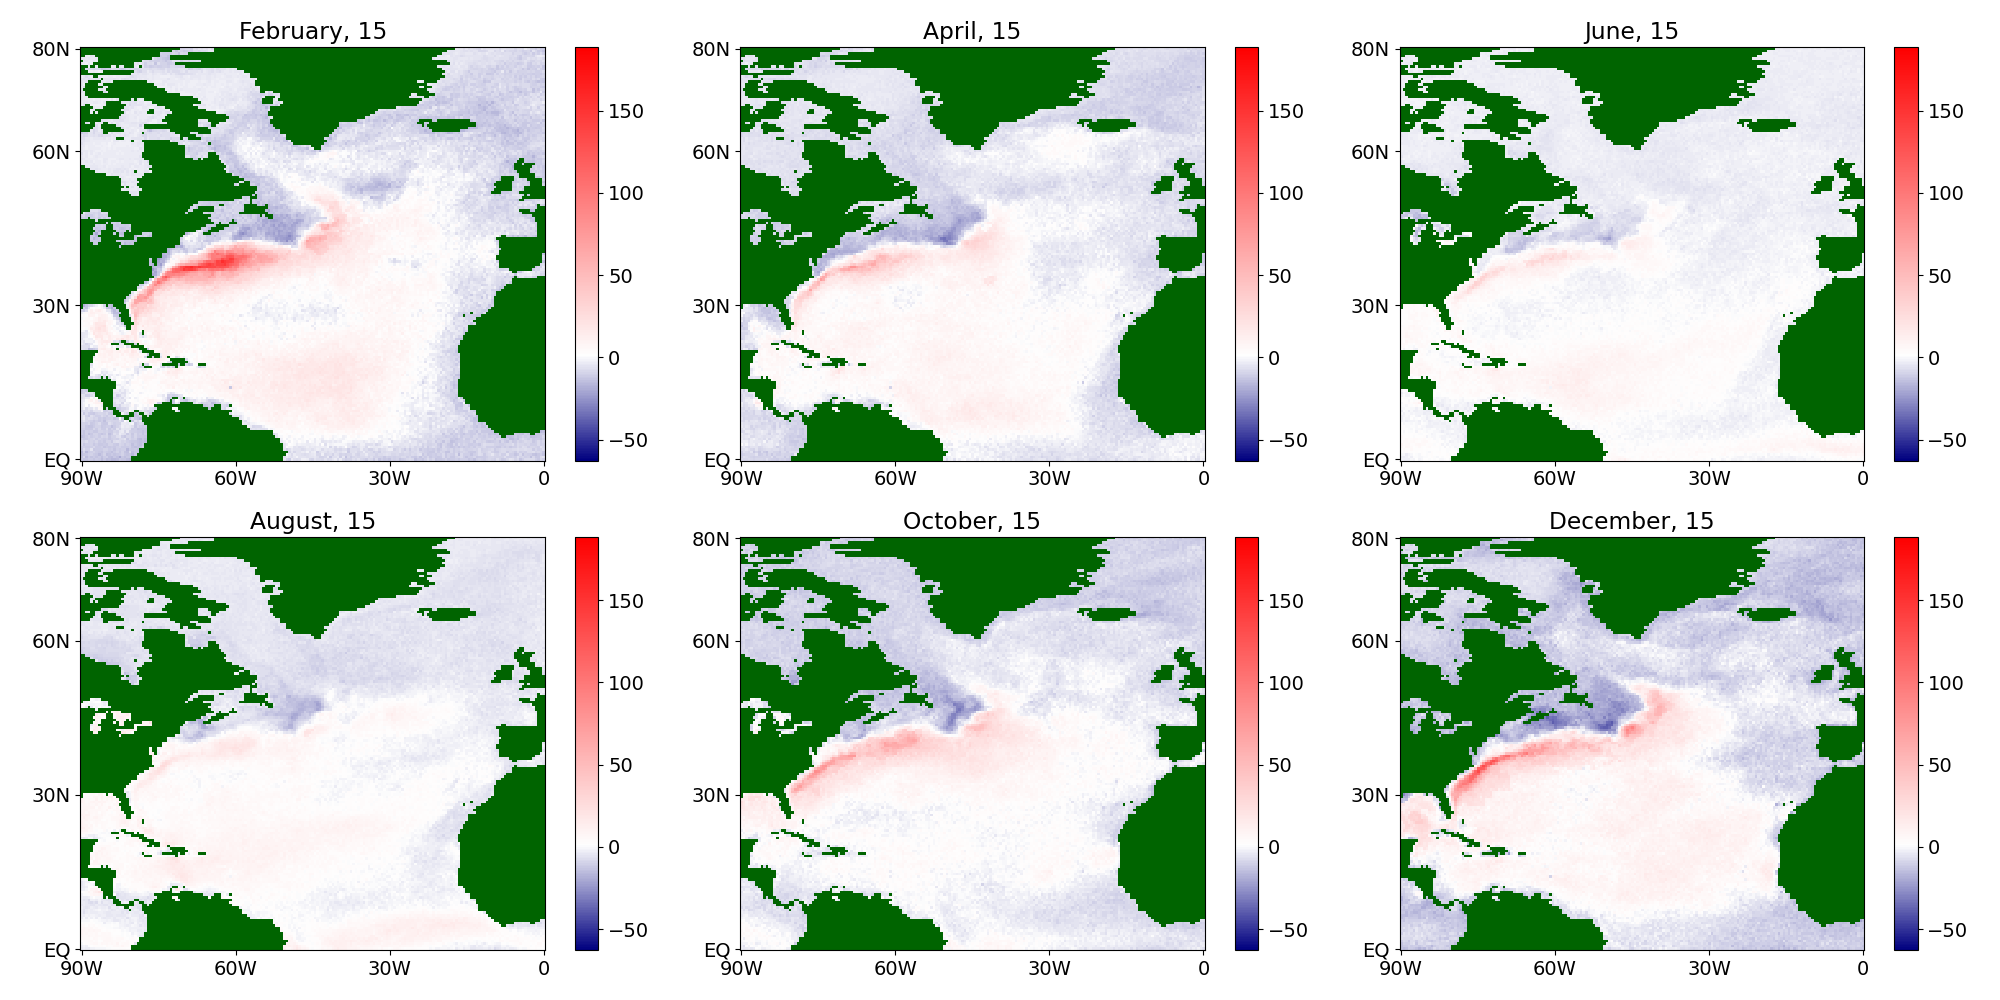
\includegraphics[width=\textwidth]{A_lat_mean_year}}\\
	b)
	
	\caption{Значения коэффициента сноса для явного (a) и скрытого (b) потоков в течение среднего года, $1979$--$2021$ гг.} 
	\label{fig:ab_mean_year}
\end{figure}

С точки зрения геофизики, эти районы показывают преобладание явного потока тепла (рис.~\ref{fig:ab_mean_year}a), то есть непосредственно разности температур вода--воздух и их динамику во времени с преимущественным направлением внутри океана: в зимние месяцы хорошо видна зона основного течения Гольфстрима. Наоборот, поток из атмосферы (нагрев океана) наблюдается в районе Лабрадорского течения. В переходный период (апрель--май) зона передачи тепла в атмосферу уменьшается (температуры выравниваются), а холодное Лабрадорское течение по-прежнему забирает тепло из атмосферы, имея минимальную динамику вдоль Атлантического побережья. В летние месяцы все процессы выравниваются, и наблюдаемые явления возобновляются только в ноябре--декабре. При этом <<холодная>> зона в районе Лабрадора остается, хотя контраст с окружающим воздухом уменьшается.

Все эти процессы гораздо заметнее для скрытых потоков (рис~\ref{fig:ab_mean_year}b), для которых передача тепла (влаги) из атмосферы в океан в северных широтах происходит практически на протяжении всего года, так как нагретая и влажная атмосфера при столкновении с относительно холодным океаном сохраняет стационарное состояние в обширных областях. Только вдоль Северо-Атлантического течения и Скандинавского побережья прослеживается слабый положительный скрытый поток. 

\section{Коэффициент диффузии}
Для матричного коэффициента диффузии $b(t,X)$ также были построены оценки за весь рассматриваемый период с шагом в $1$ день. Пример для одного из дней февраля $2022$ года приведен на рисунке~\ref{fig:b_example}. Расположение оценок на картах соответствует структуре матрицы $b$, приведенной в формуле~\eqref{eq:b_coeff_est}: левый верхний квадрат отвечает элементу $b_{11}(t,X)$ и т.д. Для отображения значений на карте используется красный цвет различной интенсивности.

\begin{figure}[h!]
	\centering
	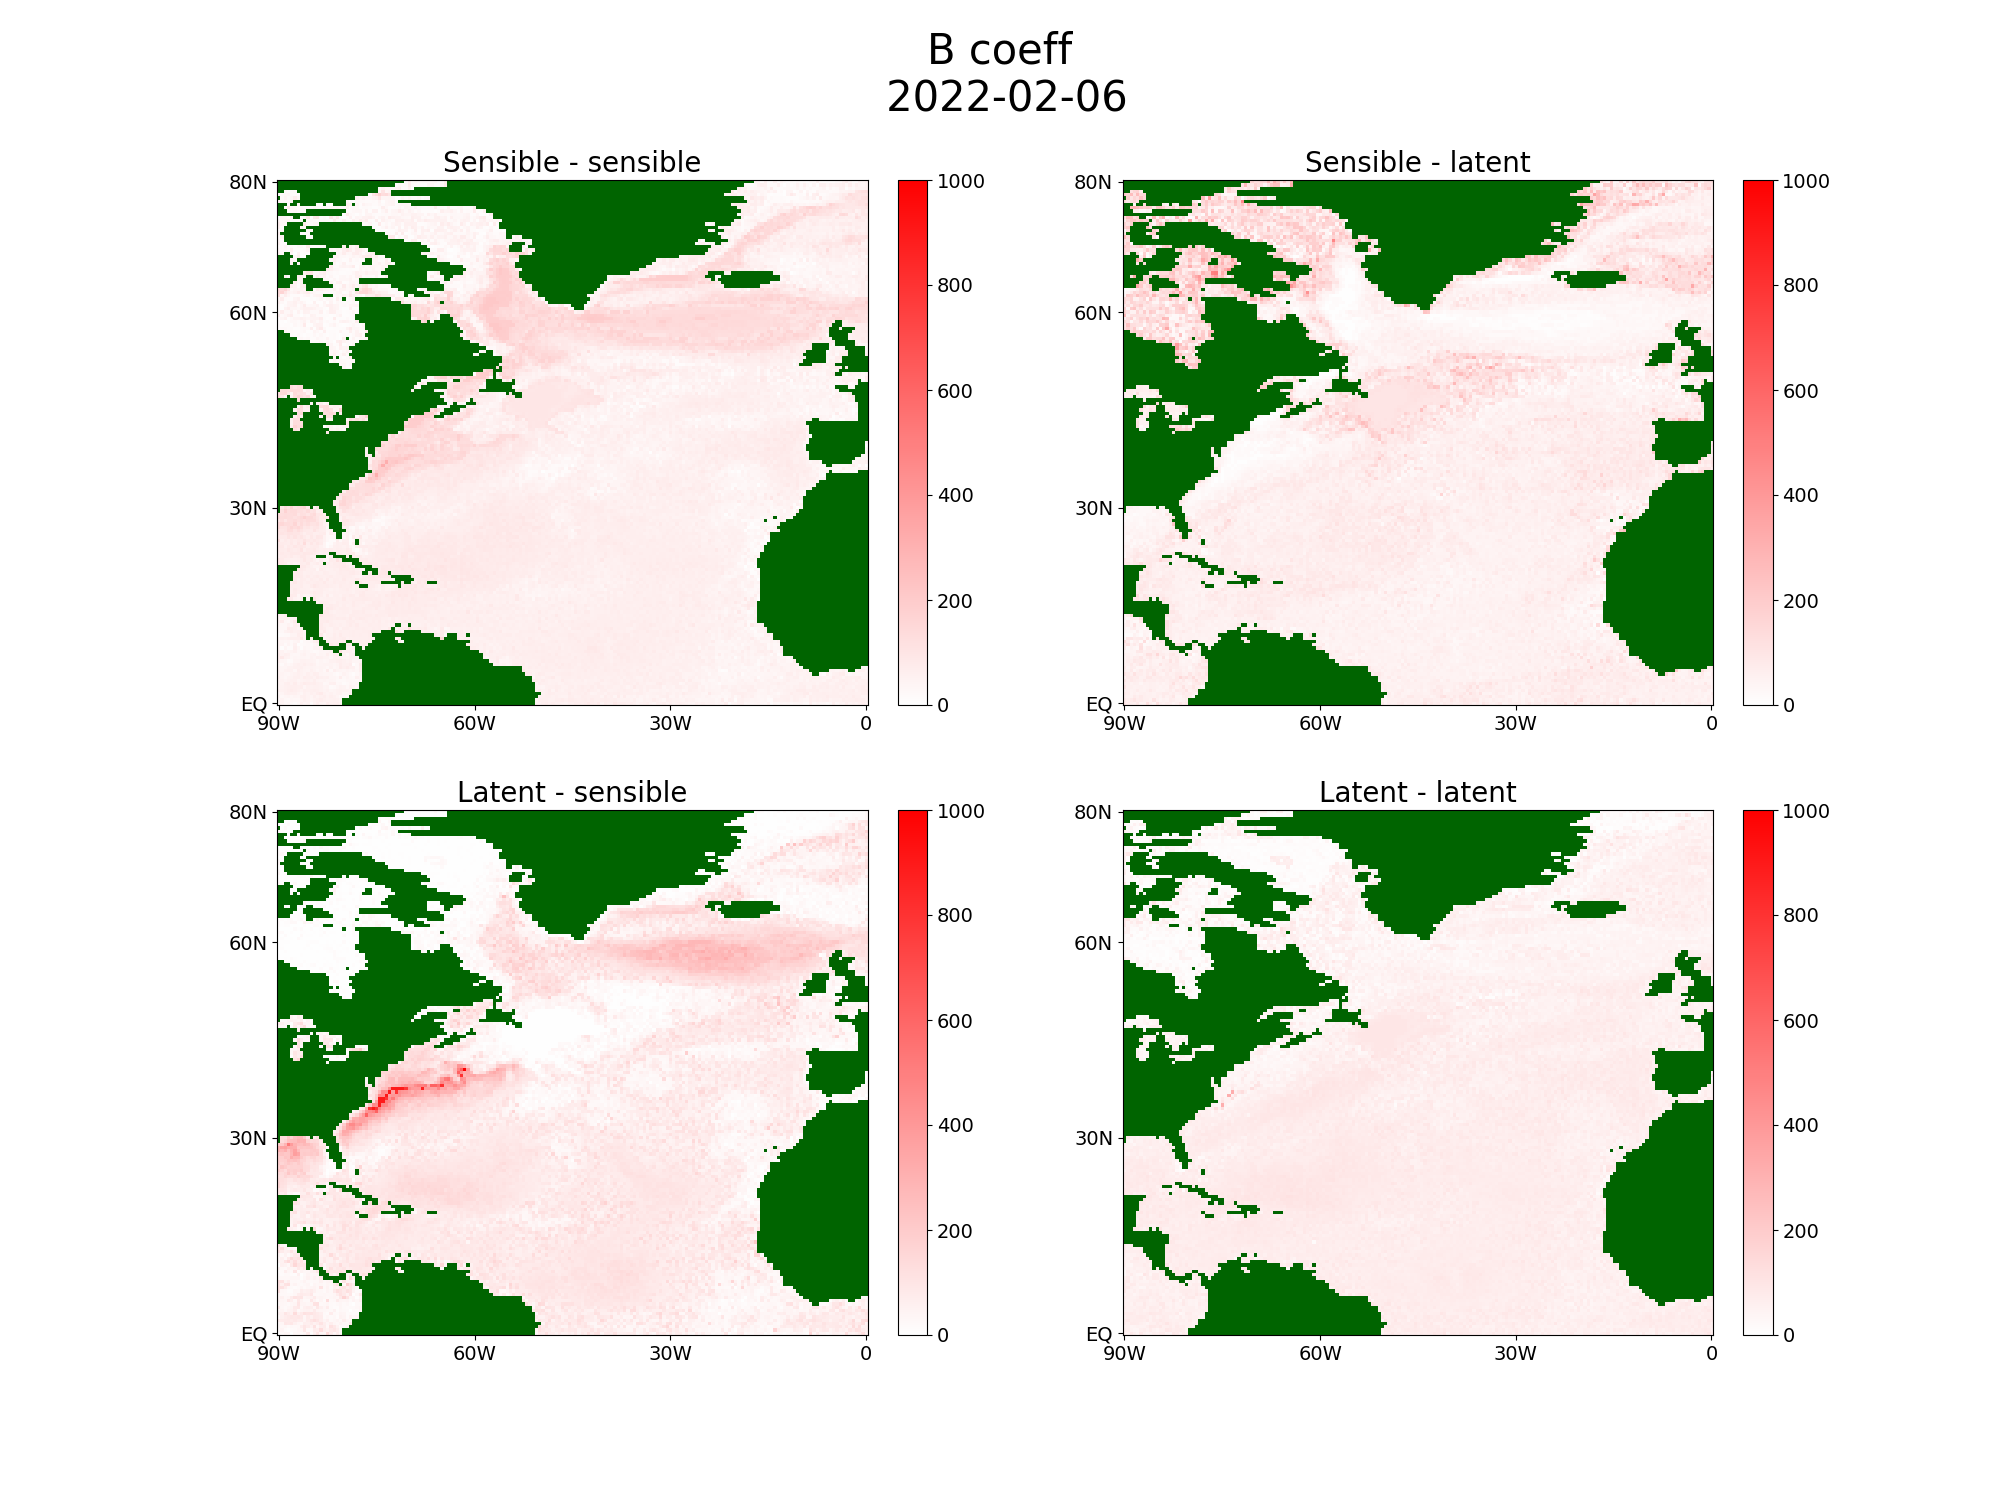
\includegraphics[width=0.8\textwidth]{B_15742}
	\caption{Пример оценок коэффициента диффузии} 
	\label{fig:b_example}
\end{figure}

% 	Цветовая шкала меняется от $0$ (белый цвет) и далее используется красный диапазон для положительных значений.
% 	Отрицательные значения, напомним, встречались при взятии матричного корня на побочной диагонали, как комплексные значения, для которых сохранялись только действительная часть числа.
Яркость цвета в конкретной точке соответствует удаленности значения от нуля. При этом на цветовой шкале максимум выбран равным $1000$ для максимальной наглядности. Более высокие значения наблюдались менее чем в $0.1\%$ случаев, поэтому во избежание излишнего размывания цветовых диапазонов при визуализации обозначались максимальным допустимым значением из диапазона и соответствующим цветом. Темно-зеленым цветом обозначена суша. На рисунке~\ref{fig:b_mean_year} изображены оценки $b_{11}(t,X)$ (рис.~\ref{fig:b_mean_year}а)) и $b_{22}(t,X)$ (рис.~\ref{fig:b_mean_year}б)) в выбранные дни за средний год.


\begin{figure}[!h]
	\centering
	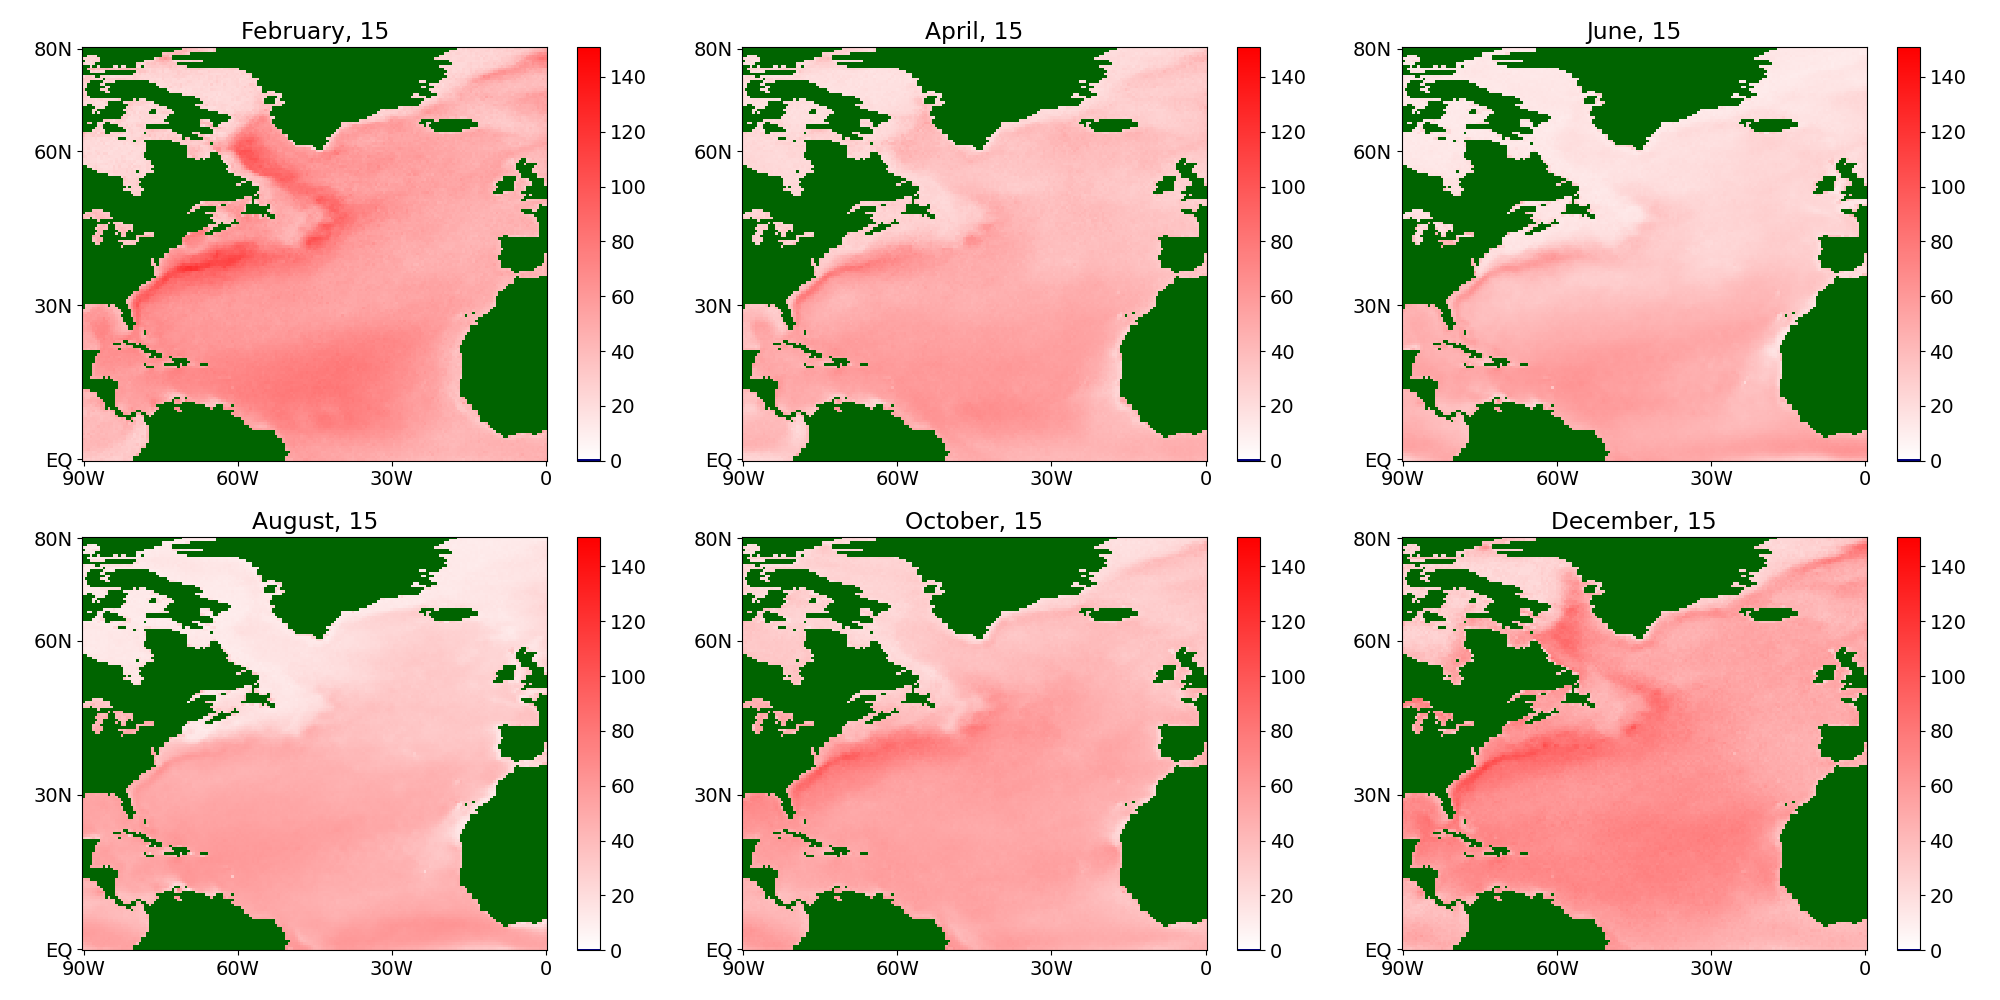
\includegraphics[width=\textwidth]{B11_mean_year}\\
	а)
	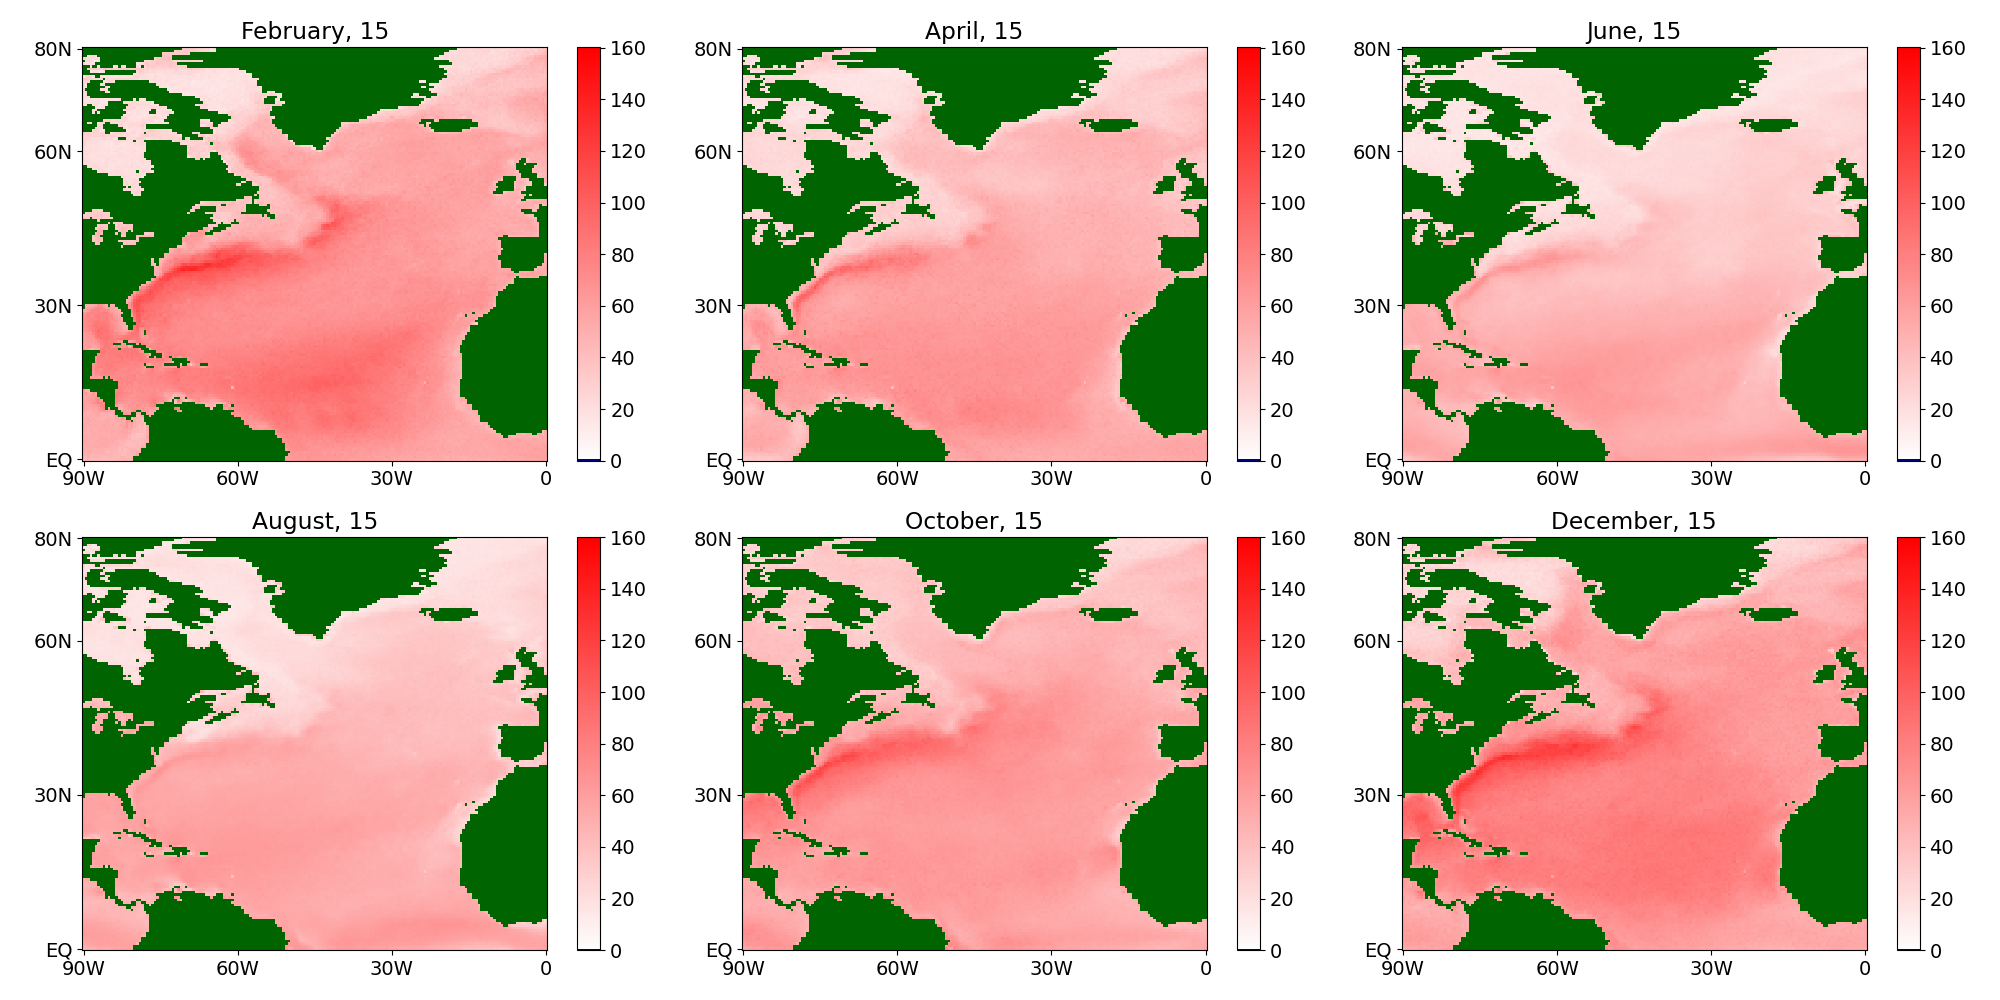
\includegraphics[width=\textwidth]{B22_mean_year}
	\\
	б)
	
	\caption{Оценки коэффициента $b_{11}(t,X)$ для явного потока (a) и коэффициента $b_{22}(t,X)$ для скрытого потока (b) в течение среднего года}
	\label{fig:b_mean_year}
\end{figure} 

По результатам анализа многолетних данных установлено, что для коэффициента $b(t,X)$ явно прослеживается обратная зависимость для элементов $b_{12}(t,X)$ и $b_{21}(t,X)$: на картах более светлые области для одного являются более яркими для второго, и наоборот. Для оценок $b_{11}(t,X)$ и $b_{22}(t,X)$ характерны те же сезонные свойства, что и для коэффициента сноса $a(t,X)$: в зимние периоды абсолютные значения границ диапазона между квантилями порядка $0.1$ и $0.9$ больше, чем в летние месяцы (см. табл.~\ref{tab:quantiles_b}). Наиболее высокие значения диффузионной составляющей встречаются в центральных и южных районах Cеверной Атлантики. 

\begin{table}[h!]
	\centering
	\caption{Диапазоны значений в летний и зимний периоды между квантилями уровня $0.1$ и $0.9$ для $b_{11}$ и $b_{22}$}
	\begin{tabular}{|c|c|c|c|c|}
		\hline
		Период & 1979-1989гг. &  1989-1999гг. & 1999-2009гг. & 2009-2019гг.\\
		\hline
		$b_{11}$, лето & $[10.5, 59.1]$ & $[10.5, 58.5]$ & $[10.8, 60.7]$ & $[10.8, 61.4]$\\ 
		\hline
		$b_{11}$, зима & $[18.5, 76.0]$ & $[18.8, 78.3]$ & $[19.8, 81.9]$ & $[18.5, 78.5]$\\ 
		\hline
		$b_{22}$, лето & $[14.1, 63.5]$ & $[14.0, 63.9]$ & $[14.9, 66.2]$ & $[14.8, 66.8]$\\ 
		\hline
		$b_{22}$, зима & $[22.6, 86.0]$ & $[22.4, 88.6]$ & $[24.3, 90.3]$ & $[22.4, 91.1]$\\ 
		\hline
	\end{tabular}
	\label{tab:quantiles_b}
\end{table}


Матрица диффузии показывает области, где преобладает непосредственное взаимодействие океана с атмосферой (при небольших значениях коэффициента сноса). Отметим, что обратная соотношение между данными величинами, то есть небольшая диффузия и значительный коэффициент сноса,  характеризует перенос потока тепла не только в атмосферу, но и внутри океана.

В зимние месяцы выделяется <<красная>> зона вдоль основного течения Гольфстрима и к северу от $40^\circ$~с.ш. (см. рис.~\ref{fig:b_mean_year}б), %также \degree из gensymb
где сильны взаимодействия как явного так и скрытого потоков за счет разности тепла и влаги между океаном и атмосферой. Также надо отметить роль сильных ветров в зимние месяцы (шторм-треки циклонов), которые в значительной степени формируют этот обмен. С учетом того, что квадрат коэффициента диффузии дает оценки энергобаланса между океаном и атмосферой, на приведенных картах можно выделить области с наибольшей энергоактивностью, прежде всего, для графиков зависимости между скрытым и явным потоками. В качестве энергоактивных областей, по классификации Г.И.Марчука~\cite{marchuk1989}, можно выделить Ньюфаундленский и Норвежский полигоны. 

\section{Взаимосвязь динамической и диффузионной составляющих процесса}
В данном разделе рассматривается взаимосвязь коэффициентов сноса и диффузии СДУ Ито~\eqref{eq:Ito} для явных и скрытых потоков тепла. 

Сначала рассмотрим поведение выборочного коэффициента корреляции Пирсона: для двух выборок $x = (x_1, \dots, x_m)$ и $y = (y_1, \dots, y_m)$ размерности $m$ он определяется следующим образом
\begin{equation}
	\label{eq:Pearson}
	r_{xy} = \frac{\sum_{i=1}^{m}(x_i - \overline{x})(y_i - \overline{y}) }{\sqrt{\sum_{i=1}^{m}(x_i - \overline{x})^2 \sum_{i=1}^{m}(y_i - \overline{y})^2}}.
\end{equation}

Рассматривается поведение оценок $(a_1, a_2)$ и $(b_{11}, b_{22})$
в режиме скользящего окна ширины $14$ дней, то есть в качестве векторов $x$ и $y$ из \eqref{eq:Pearson} выступают наборы $(a_1(t), a_1(t+1), \dots, a_1(t+14)), (a_2(t), a_2(t+1), \dots, a_2(t+14))$ и $(b_{11}(t), b_{11}(t+1), \dots, b_{11}(t+14)), (b_{22}(t), b_{22}(t+1), \dots, b_{22}(t+14))$, а размерность векторов $m=14$.

\begin{figure}[!h]
	\centering
	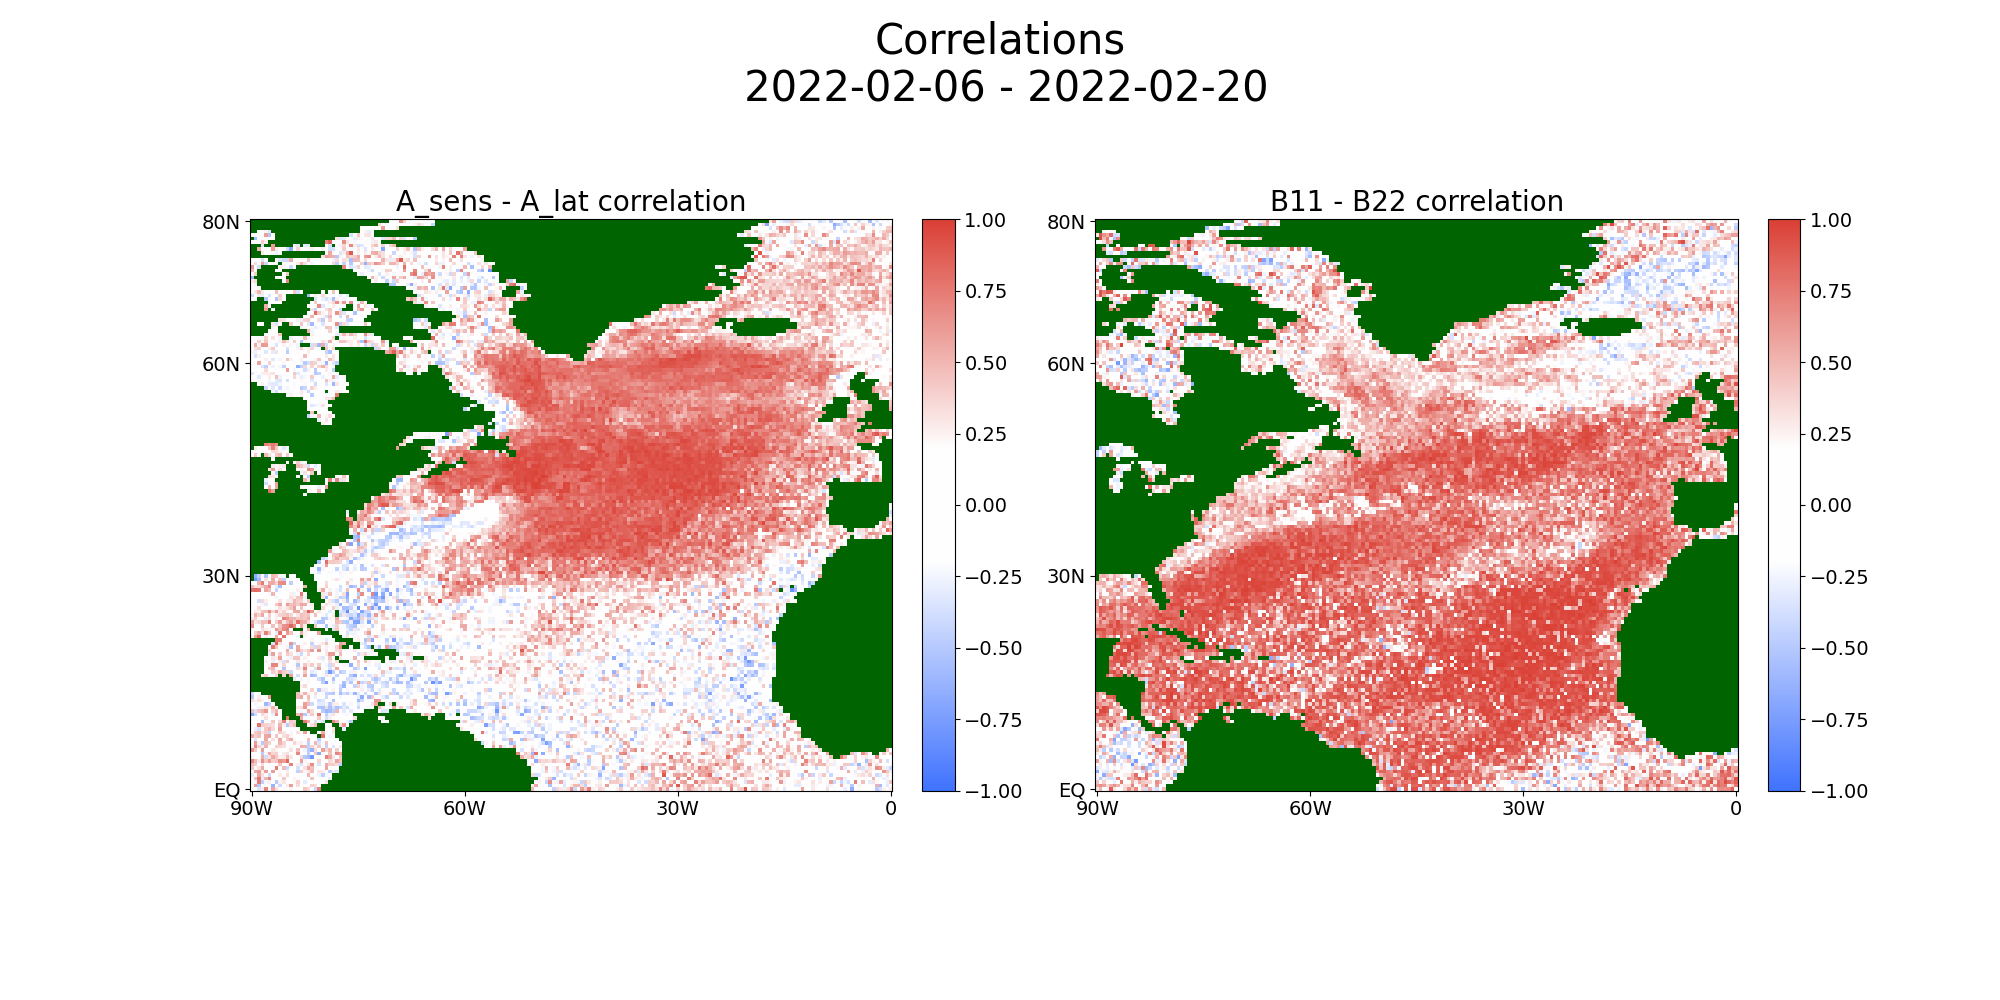
\includegraphics[width=\textwidth]{C_15742}
	\caption{Пример корреляций между оценками коэффициентов сноса (карта слева) и диффузии (карта справа)}
	\label{fig:c_example}
\end{figure}

На рисунке~\ref{fig:c_example} показан пример полученной корреляции для коэффициентов сноса (карта слева) и диффузии (карта справа) явных и скрытых потоков. Цветовая шкала меняется от синего при отрицательных значениях до до красного при положительных, белый цвет соответствует оценкам, близким к $0$. Яркость цвета в конкретной точке соответствует удаленности значения от нуля. Минимум и максимум шкалы естественным образом равны $-1$ и $1$, соответственно. Темно-зеленым цветом, как и ранее, обозначена суша. Для коэффициента сноса в области Саргассова моря периодически наблюдаются области с отрицательной корреляцией, для диффузиозной составляющей же это обыкновенно области Норвежского моря, Гудзонова залива и моря Баффина. В зимние месяцы корреляция двух компонент коэффициента сноса существенно положительна в широком коридоре вдоль течения Гольфстрима, а в летние месяцы коридор положительных значений существенно сужается. Отрицательные значения встречаются редко и визуально равномерно распределены по всей карте, и встречаются как в летние, так и в зимние периоды.

\begin{figure}[h!]
	\centering
	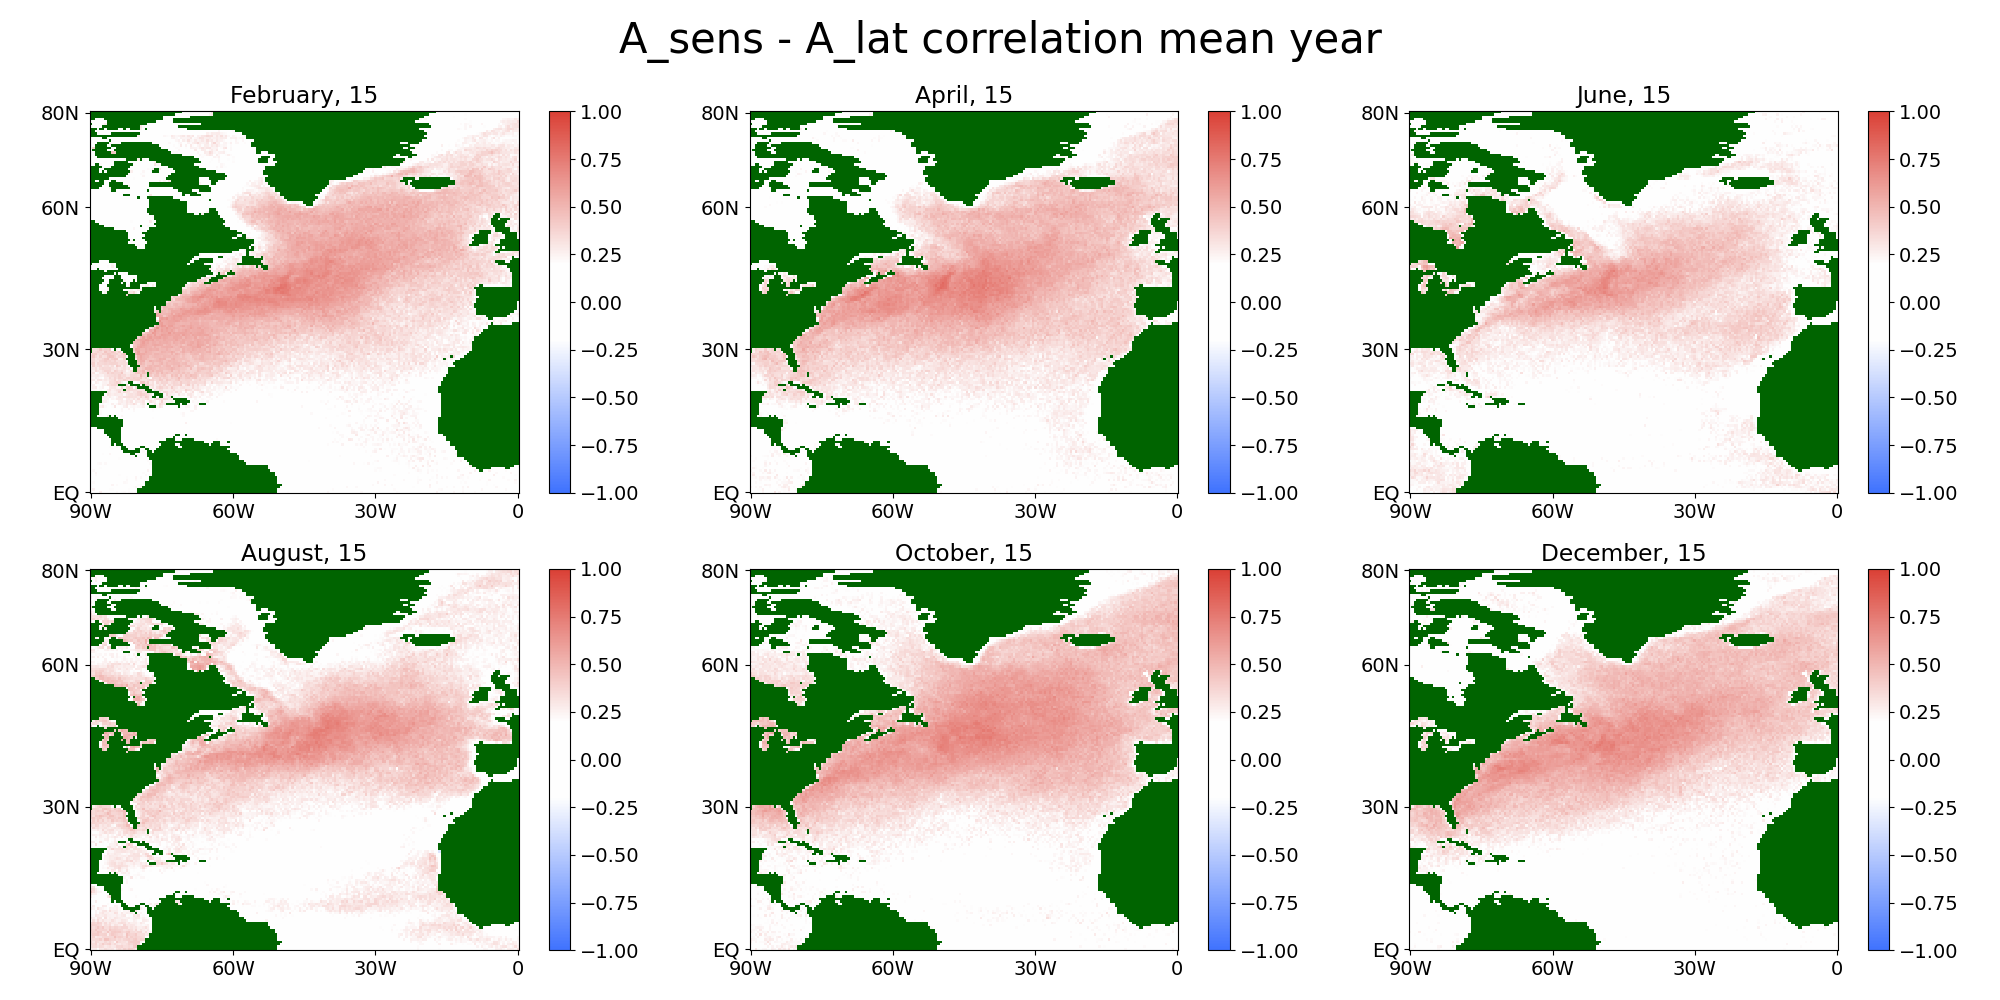
\includegraphics[width=\textwidth]{C_0_mean_year}
	\caption{Корреляции между $a_1$ и $a_2$ в течение среднего года}
	\label{fig:c0}
\end{figure}

\begin{figure}[h!]
	\centering
	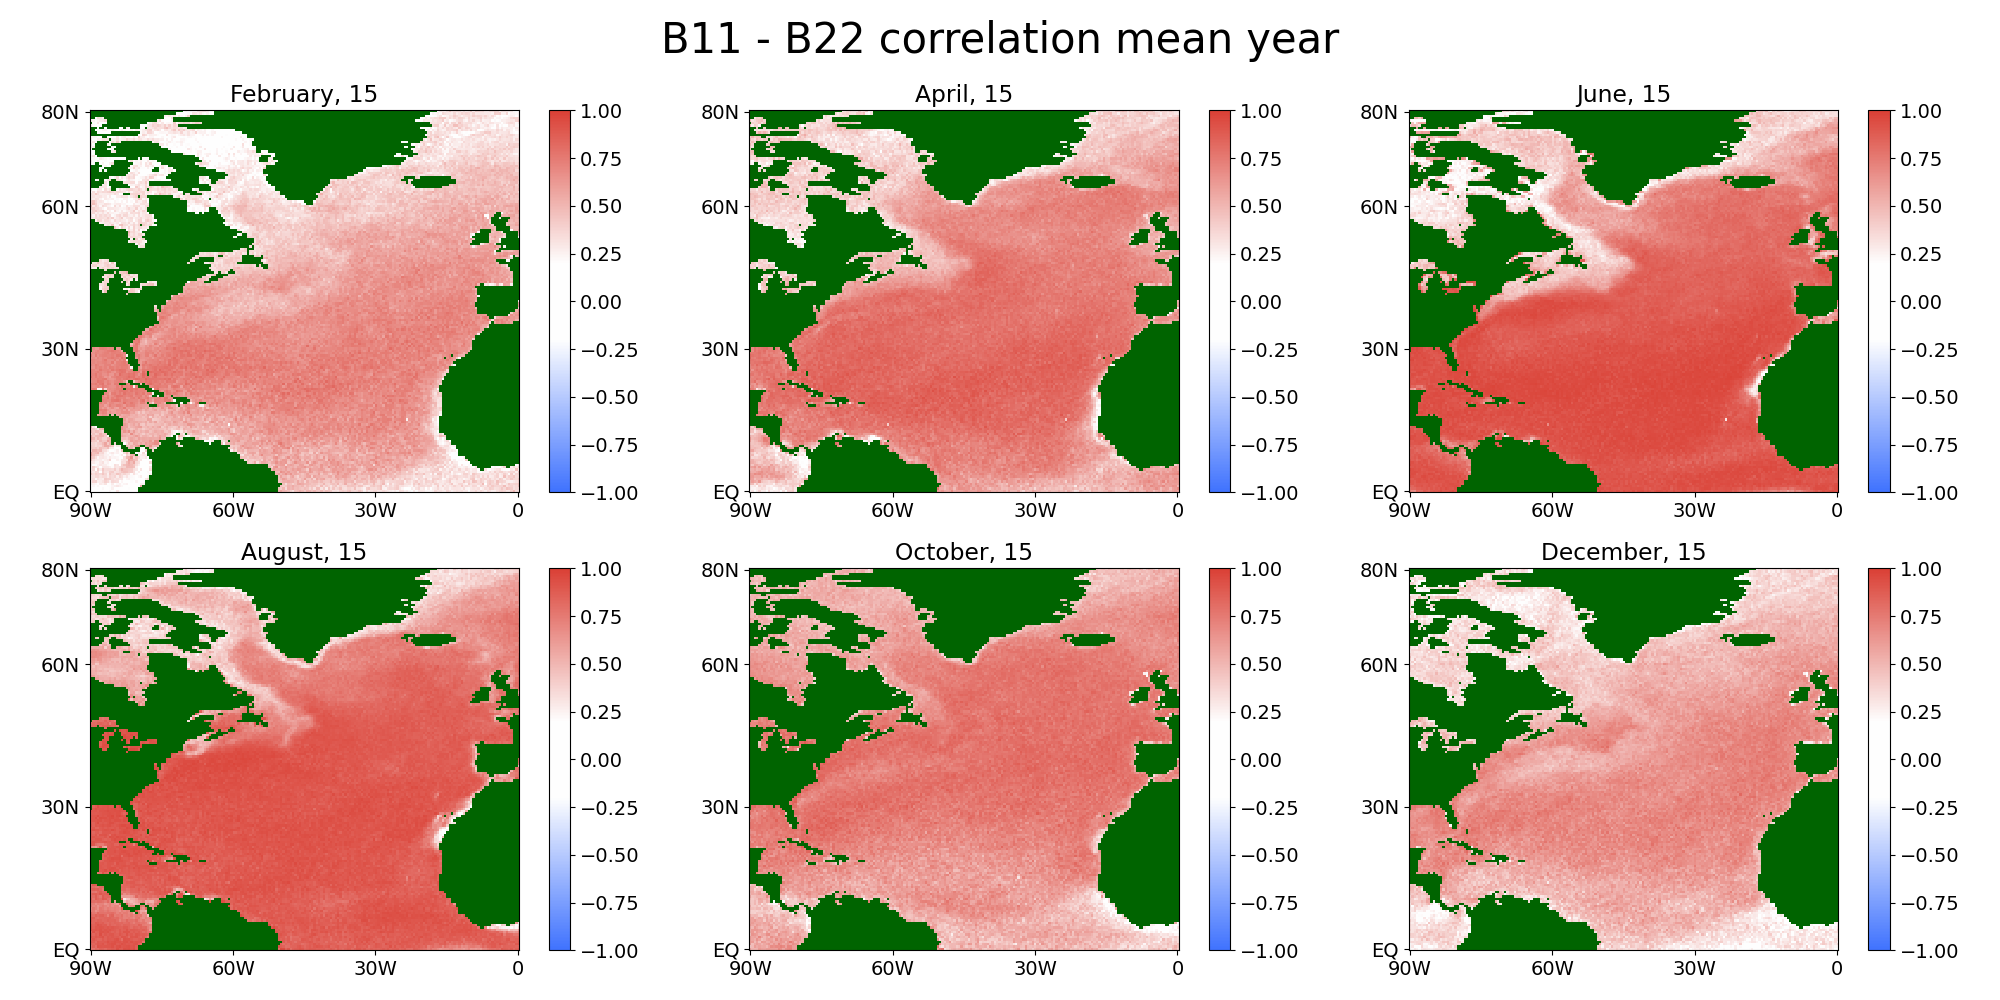
\includegraphics[width=\textwidth]{C_1_mean_year}
	\caption{Корреляции между $b_{11}$ и $b_{22}$ в течение среднего года}
	\label{fig:c1}
\end{figure}

На рисунках~\ref{fig:c0} -~\ref{fig:c1} показаны корреляции между парами $(a_1, a_2)$ и $(b_{11}, b_{22})$ в течение среднего года. Видно, что коэффициенты диффузии имеют значительно более высокий процент положительной корреллированности, при этом значения близки к $1$. Для коэффициентов сноса такая область в акватории примерно в два раза меньше по площади, значения корреляции значительно меньше. 

Очевидно, что коэффициенты сноса и диффузии оцениваются не точно. Строго получить доверительные интервалы этих оценок без дополнительных достаточно неочевидных предположений невозможно. Однако полученные коэффициенты корреляции показывают, насколько сильно эти коэффициенты связаны, возможно ли по одному из них восстановить или оценить другой. Из приведенных картинок видно, что коэффициенты диффузии в тех районах, где они близки к $1$, определены достаточно адекватно. Для коэффициентов сноса достаточно хорошо выделяются районы струйных течений. В то же время, в южной и центральной частях Северной Атлантики течения слабо заметны, и поэтому корреляция мала.

% 	\subsection{Анализ вклада динамической и диффузиозной составляющих}
Теперь рассмотрим величину $F$, отражающую соотношение между коэффициентами $a(t,X)$ и $b(t,X)$, для каждой точки сетки с координатами $(x,y)$ в момент времени $t \in [0,T]$: 
\begin{equation}
	F(x,y,t) = \frac{|a_1(x,y,t) + a_2(x,y,t)|}{\sqrt{b_{11}^2(x,y,t) + b_{22}^2(x,y,t) + b_{12}(x,y,t) + b_{21}(x,y,t)}}.
\end{equation}

Физический смысл данной величины связан с оценкой энергии потоков как внутри океана, так и при отдаче тепла в или из атмосферы. 
% 	На рисунке~\ref{fig_f_example} показан пример визуализации данной характеристики. \textcolor{yellow}{Не заменить ли его на  а-ля средний год?} 
На рисунке~\ref{fig:f_mean_year} представлено поведение рассматриваемой величины в течение среднего года.
% 	Цветовая шкала в данном случае является дискретной, в ней присутствуют $5$ цветов. Глубина цвета в каждой области одинаковая и не зависит от удаленности значения от границ соответствующего отрезка.

% 	\begin{figure}[h!]
	% 		\center{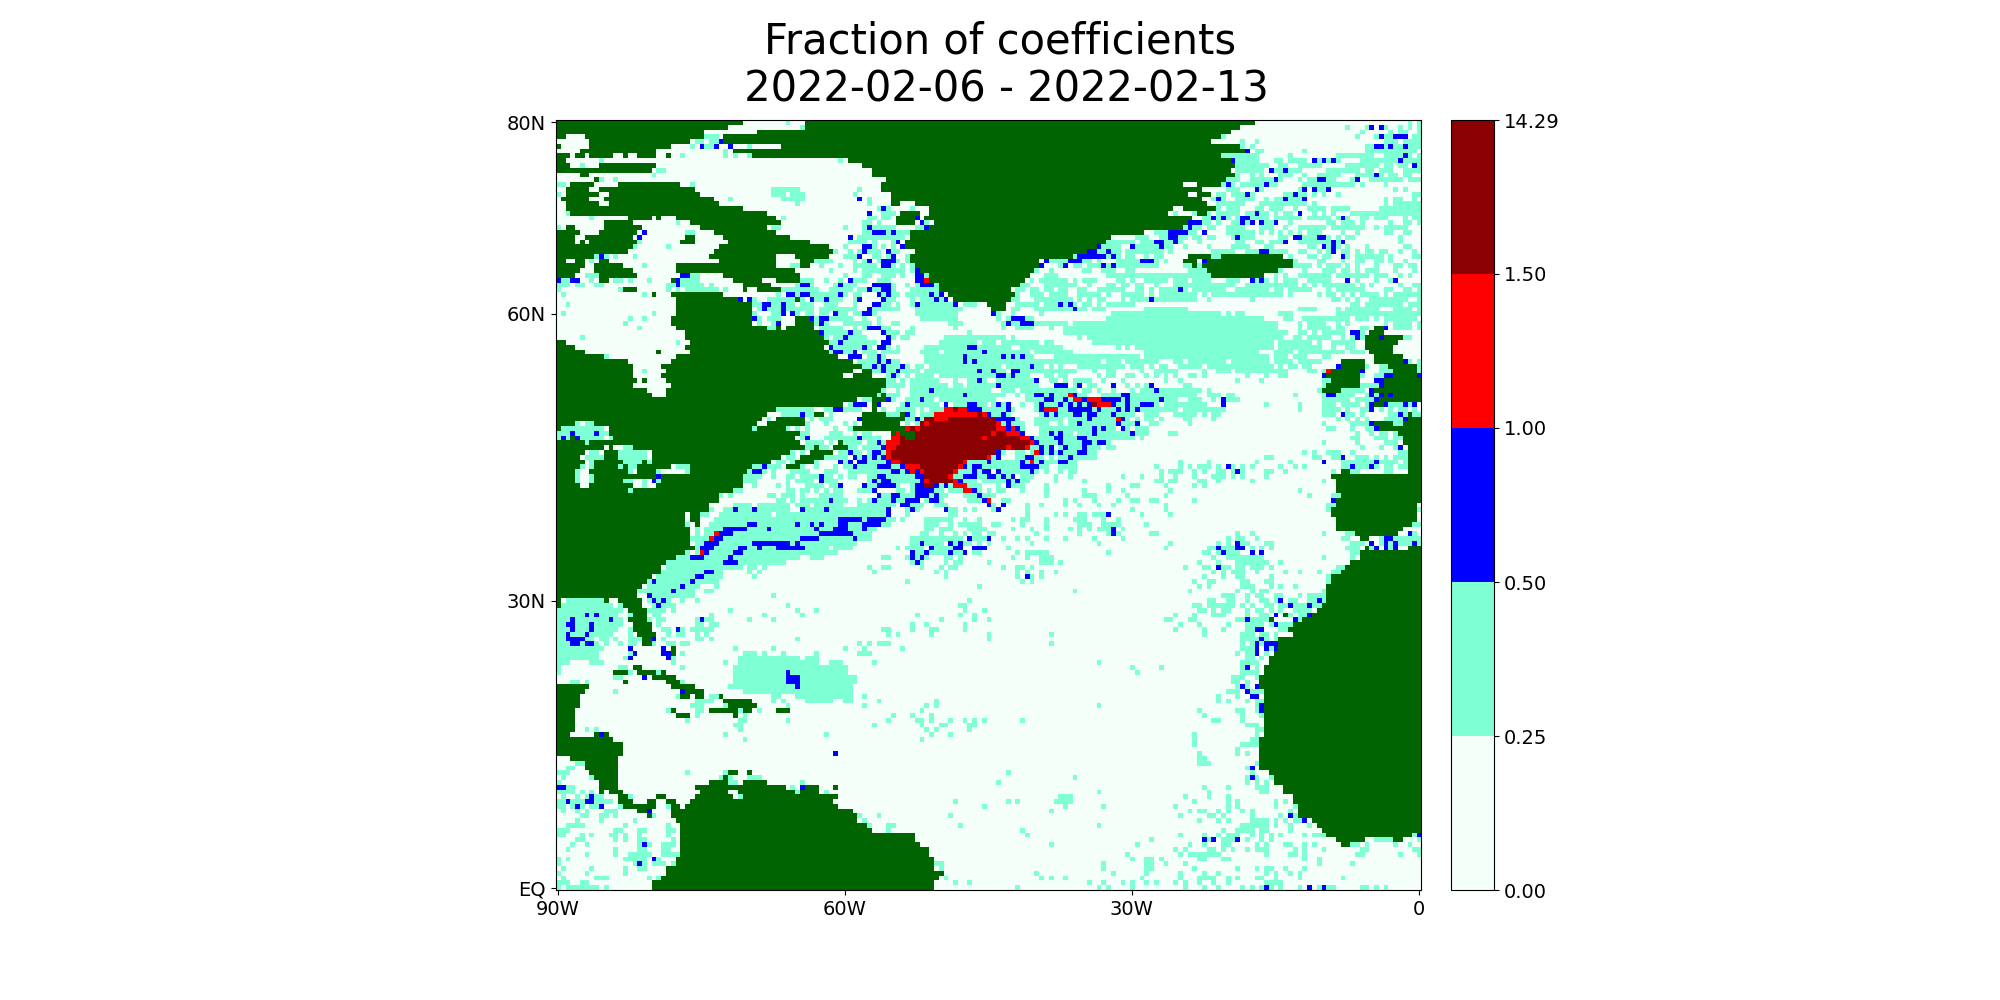
\includegraphics[width=\textwidth]{FN_15742}}
	% 		\caption{Преобладание диффузионной компоненты процесса в акватории Северной Атлантики, февраль 2022 года}
	% 		\label{fig_f_example}
	% 	\end{figure}

\begin{figure}[!h]
	\centering
	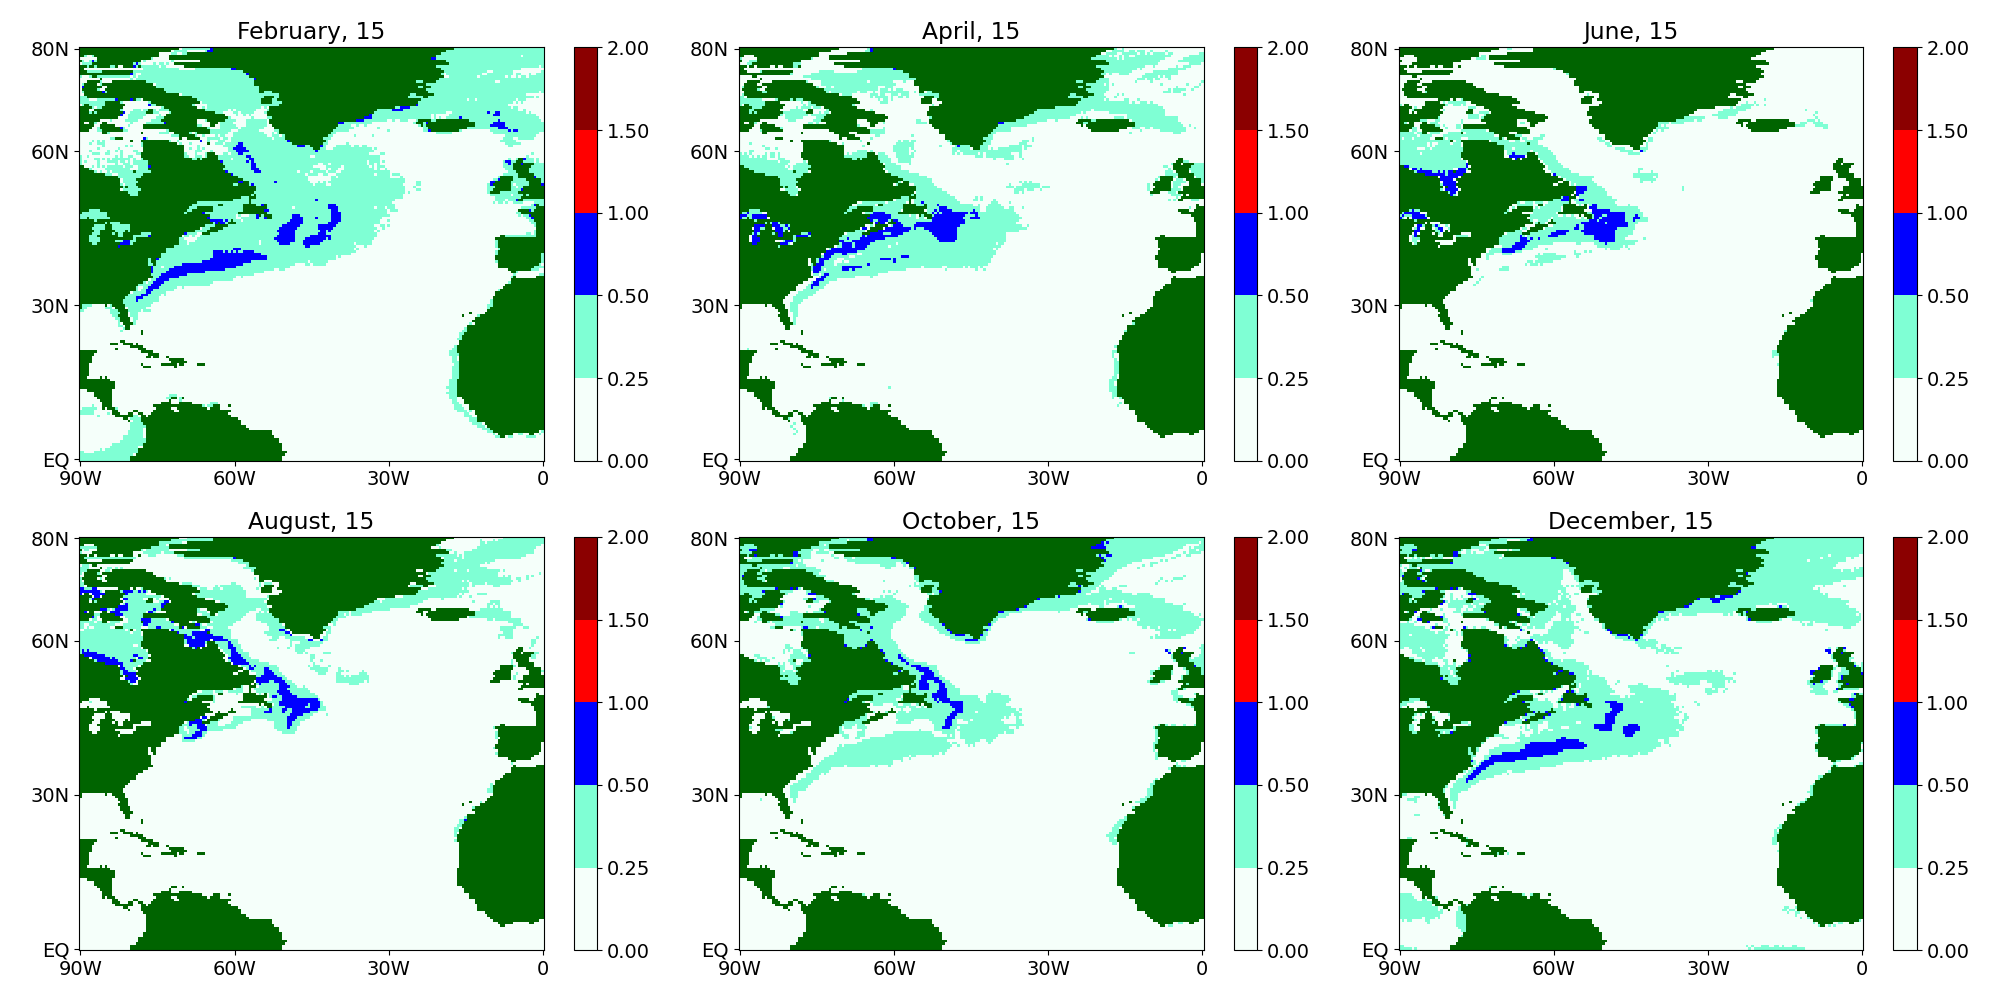
\includegraphics[width=\textwidth]{F_mean_year}
	\caption{Преобладание диффузионной компоненты процесса в акватории Северной Атлантики в течение среднего года}
	\label{fig:f_mean_year}
\end{figure}

Цветовая шкала в данном случае является дискретной, в ней присутствуют $5$ цветов. Интенсивность цвета в каждой области одинаковая и не зависит от удаленности значения от границ соответствующего отрезка. Набольшие значения величины $F$ возникают, в основном, вдоль течения Гольфстрима, а также, как и ранее, средние значения по всей акватории больше в зимний период, чем в летний. При этом в большей части акватории Северной Атлантики за весь анализируемый период преобладают значения величины $F$, не превышающие $0.5$, что говорит о преобладании диффузионной составляющей процесса. Квадрат диффузии показывает количественно вклад отдельных регионов в энергообмен океан--атмосфера, поэтому даные результаты важны с точки зрения оценок энергобаланса.

\section{Поведение характеристик коэффициентов}

В данном разделе рассмотрено поведение таких характерных величин полученных оценок, как максимум, минимум и среднее, вычисляемых по всей акватории.
Им соответствуют красный, синий и зеленый цвета на графиках далее.
% 	Отметим, что также рассматривалось поведение медианы, но оно полностью аналогично среднему, поэтому в дальнейшем не упоминается.

Сначала рассмотрим изменение этих характеристик в рамках одного года. Для примера на рисунке~\ref{fig:ab_daily} приведены данные для коэффициентов сноса и диффузии за $2021$ год для явных и скрытых потоков (верхний и нижний графики).
Среднее почти постоянно и испытывает лишь небольшие отклонения от нуля, максимумы и минимумы же обладают ярко выраженной сезонностью. Как уже отмечалось ранее, в летний период (примерно с мая по октябрь) значения оценок $a(t,X)$ и $b(t,X)$ по модулю заметно меньше, чем в остальное время года. 

\begin{figure}[!h]
	\centering
	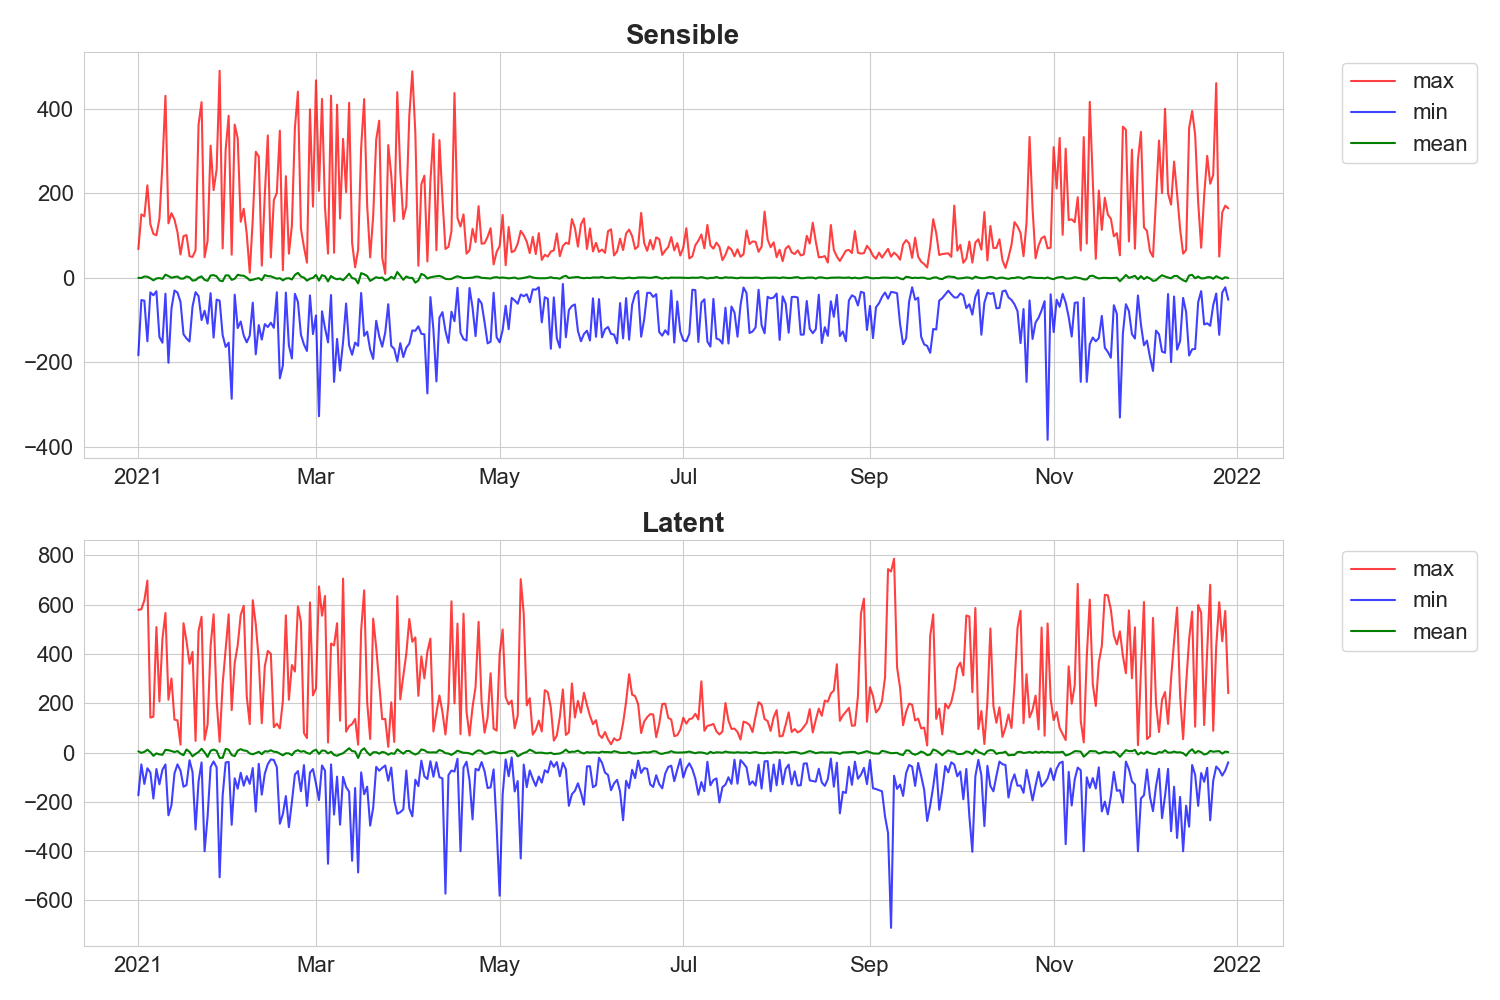
\includegraphics[width=\textwidth]{a_(15341-15705)_1}\\
	a)
	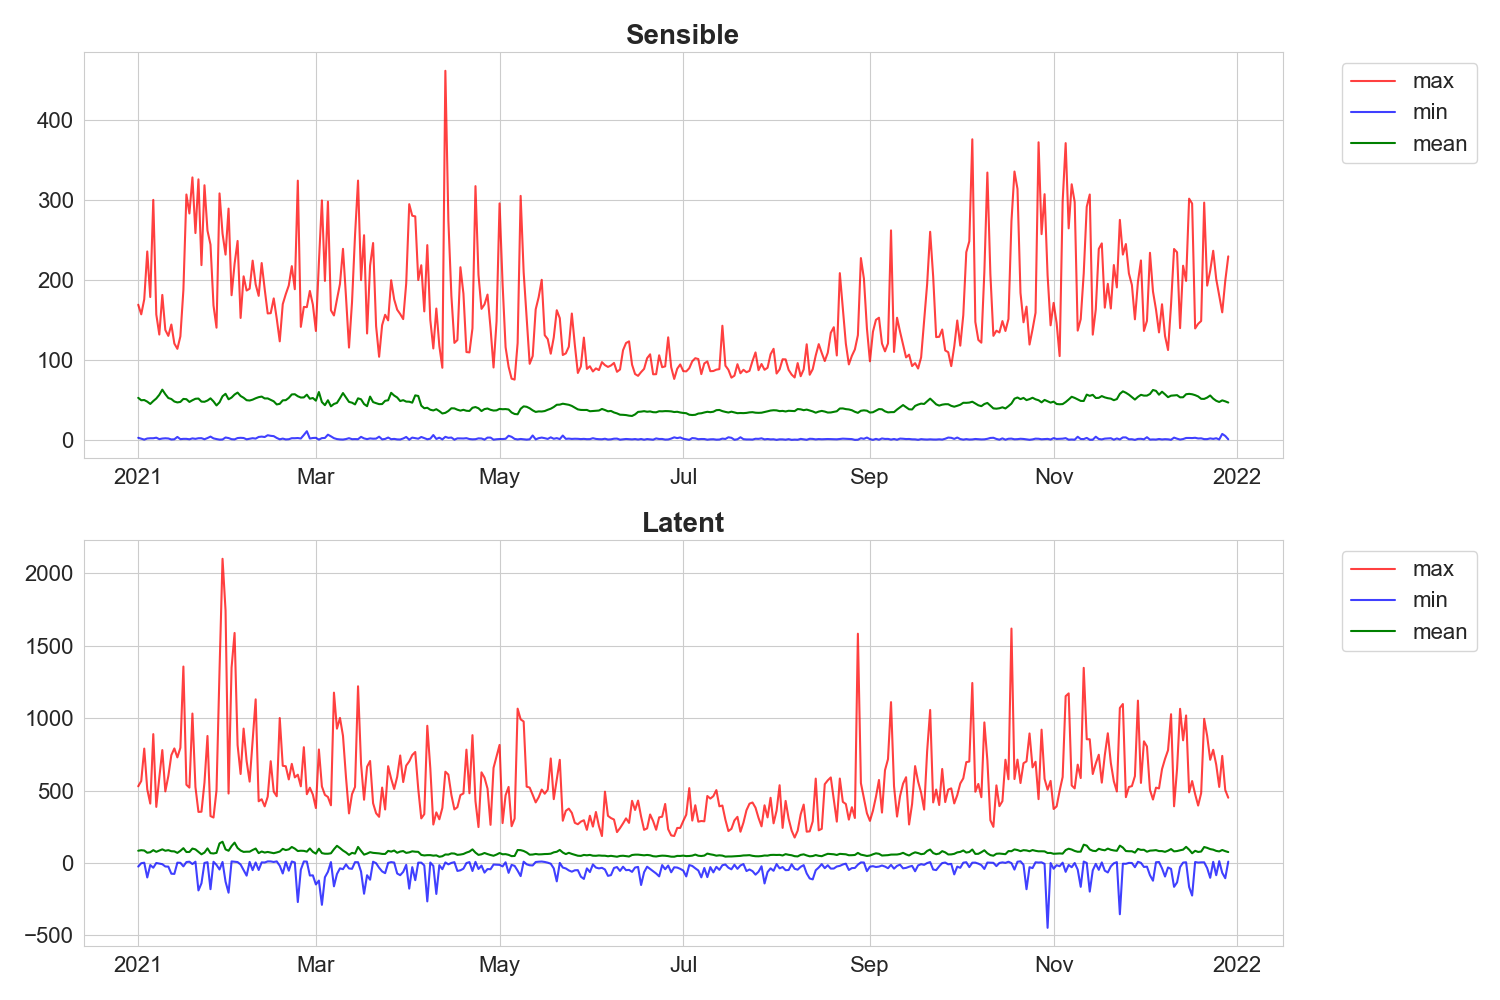
\includegraphics[width=\textwidth]{b_(15341-15705)_1}
	\\
	б)
	
	\caption{Поведение характеристик оценок коэффициентов сноса (а) и диффузии (б) для явных и скрытых потоков в течение $2021$ года с шагом в $1$ день}
	\label{fig:ab_daily}
\end{figure}

\begin{figure}[h!]
	\centering
	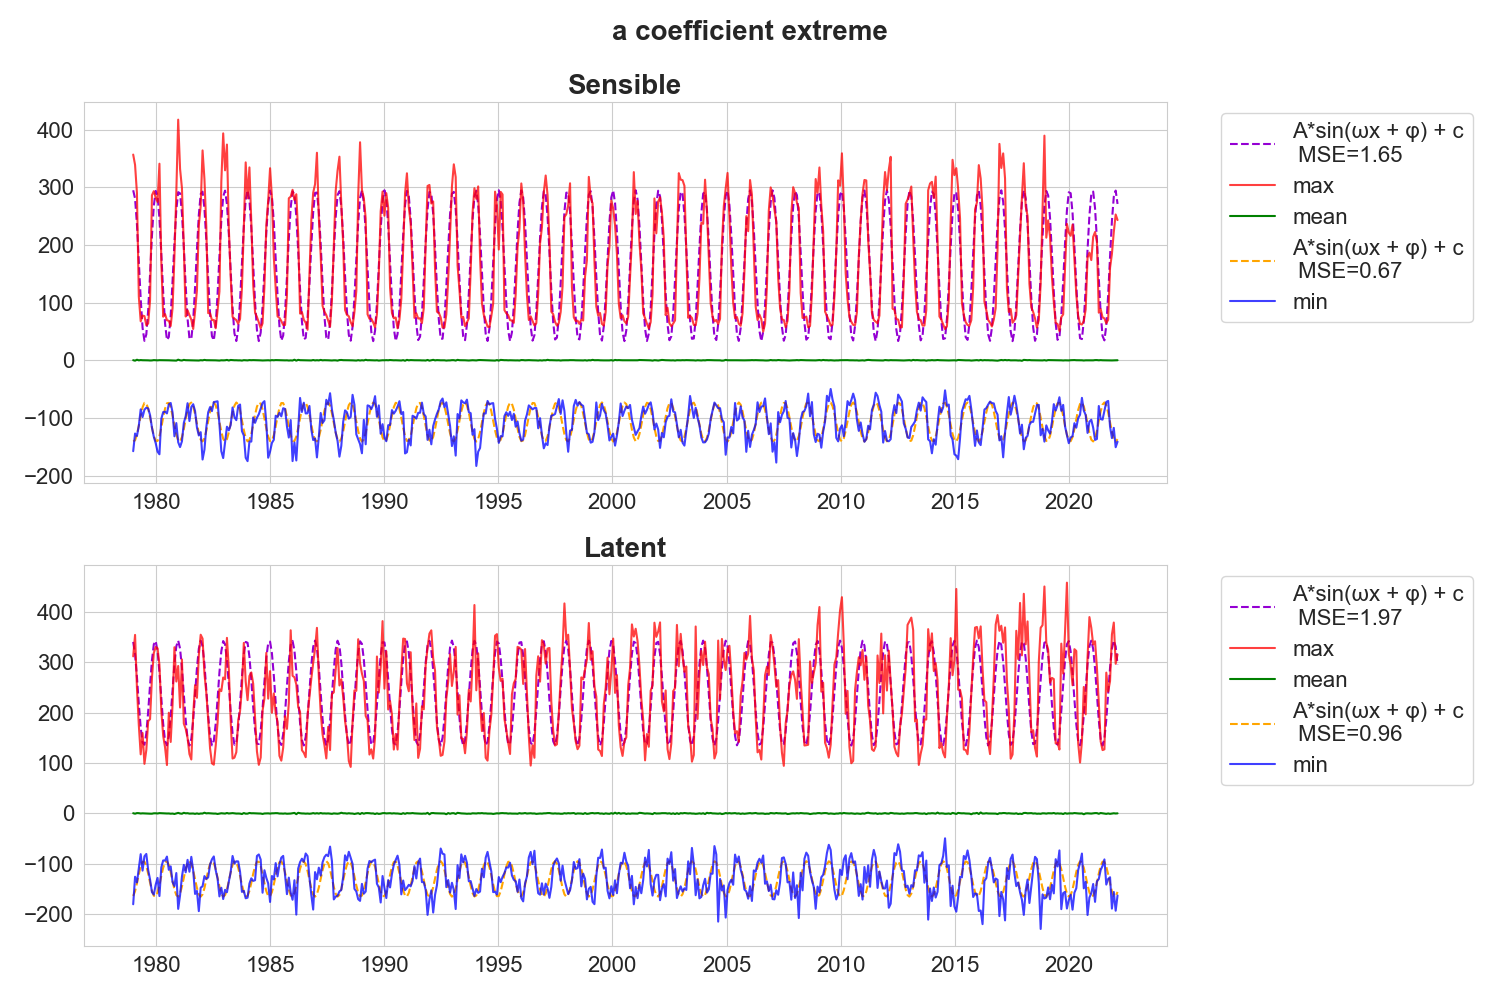
\includegraphics[width=\textwidth]{a_(1-15797)_30_fit}\\
	a)
	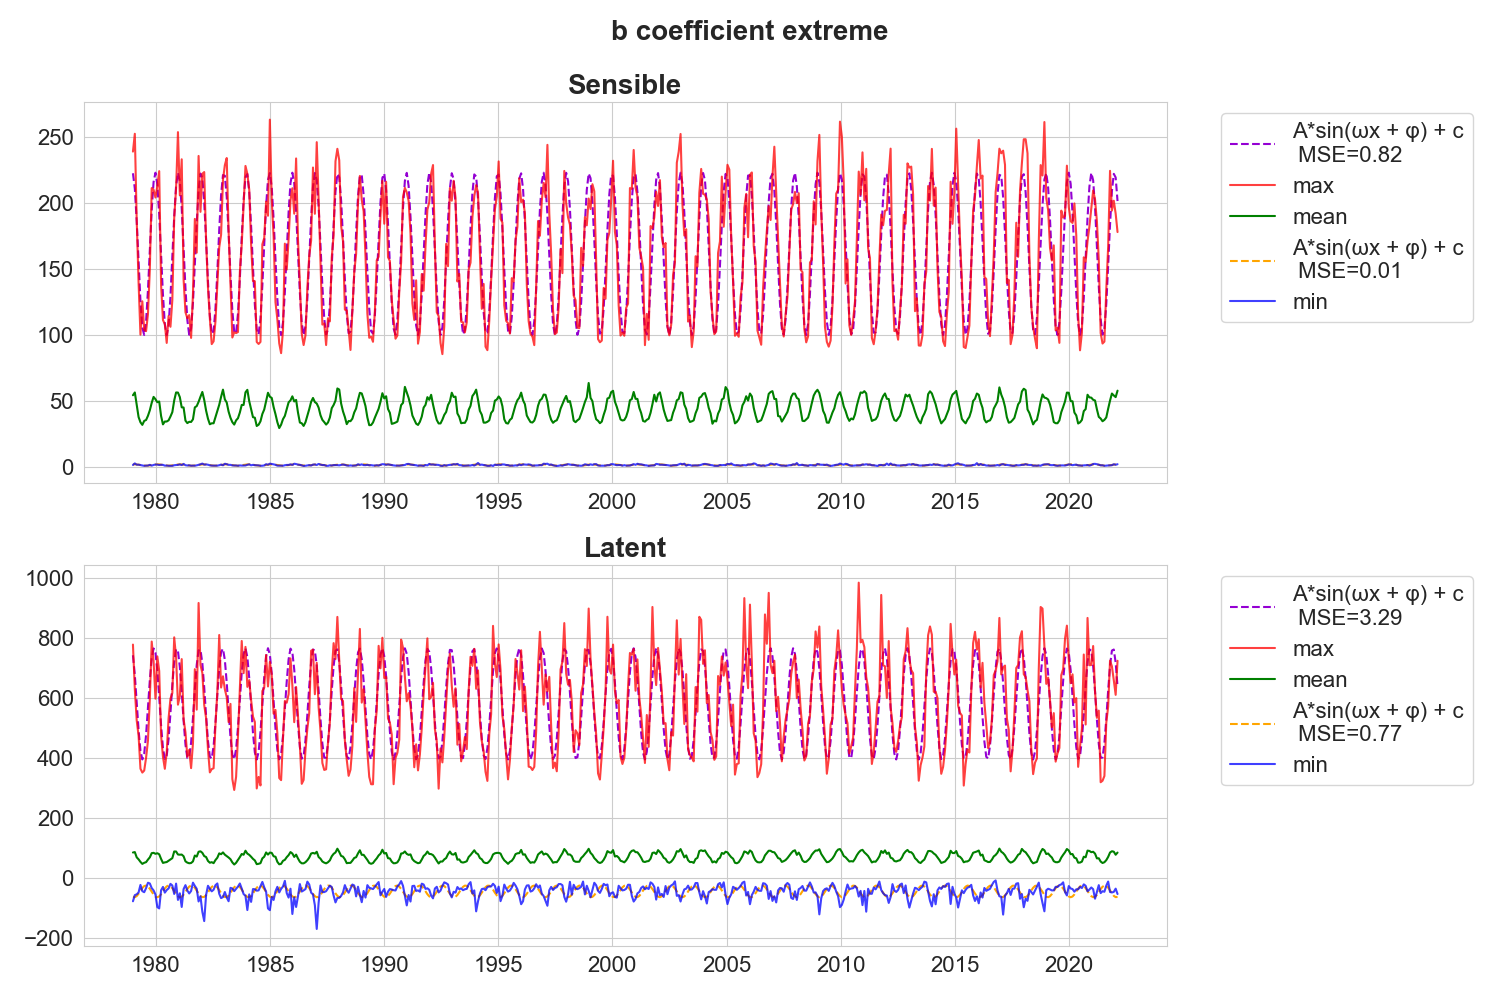
\includegraphics[width=\textwidth]{b_(1-15797)_30_fit}\\
	б)
	\caption{Поведение экстремальных характеристик оценок коэффициентов сноса (a) и диффузии (б) $1979$--$2021$~гг. с шагом в $30$ дней}
	\label{fig:ab_monthly}
\end{figure}

При рассмотрении усреднений в $30$ и $365$ дней наблюдается ярко выраженная сезонность в поведении максимумов и минимумов. Поэтому для них построена аппроксимация соответствующих кривых с помощью синусоидальной функции вида $A \cos{\omega x + \phi} + c$. На рисунке~\ref{fig:ab_monthly} представлено изменение рассматриваемых характеристик в течение $1979$--$2021$~гг., усредненных по последовательным отрезкам времени длиной $30$ дней, а также найденные функции вместе с соответствующей среднеквадратичной ошибкой приближения. С точки зрения геофизики, эти величины показывают регулярность рассматриваемого ряда в его средне- и долгосрочной изменчивости.

\begin{figure}[h!]
	\centering
	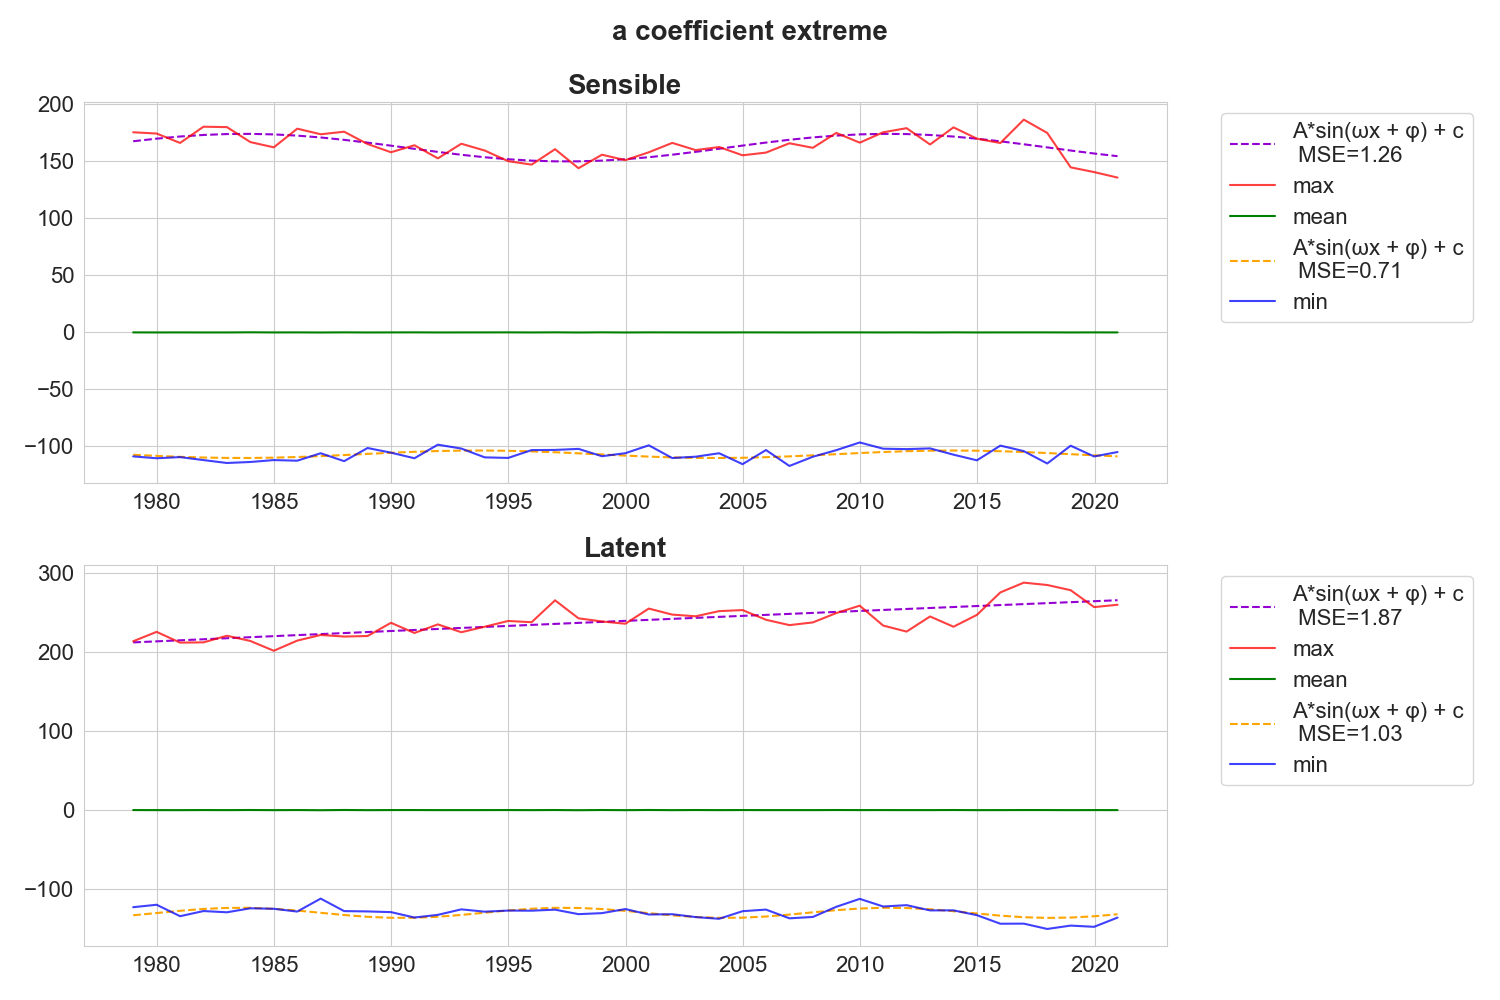
\includegraphics[width=\textwidth]{a_(1-15797)_365_fit}\\
	a)
	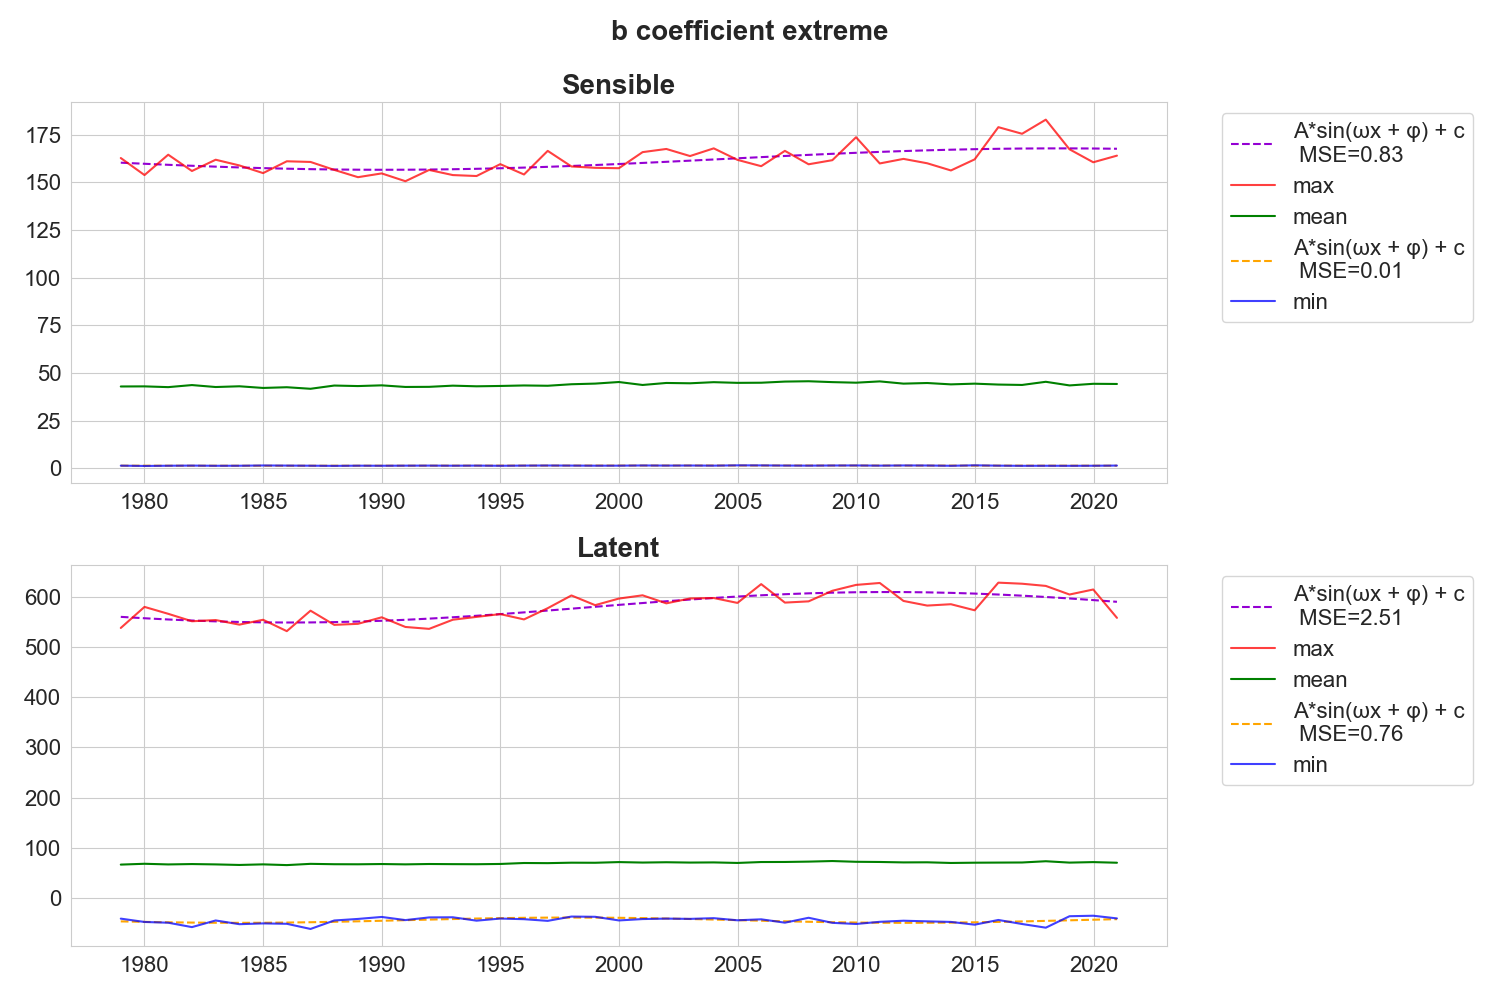
\includegraphics[width=\textwidth]{b_(1-15797)_365_fit}\\
	б)
	\caption{Поведение характеристик оценок коэффициентов сноса (a) и диффузии (б) в течение $1979$--$2021$~гг. с шагом в $365$ дней}
	\label{fig:ab_year}
\end{figure}

Рисунок~\ref{fig:ab_year} иллюстрирует изменение рассматриваемых характеристик в течение $1979$--$2021$~гг., усредненных по последовательным отрезкам времени длиной $365$ дней, а также вышеописанные приближения с помощью синусоидальной функции кривых максимума и минимума. На этих графиках сезонность выражена не так ярко. В то же время можно заметить некоторые тренды за промежуток времени длиной в $43$ года. Например, для оценок коэффициента $a(t,X)$, особенно для компоненты $a_2(t,X)$, отвечающей скрытому потоку, видно, что максимум и минимум довольно явно удаляются от линии среднего с течением времени, начиная с $2010$ года. 


\section{Вид зависимости коэффициента сноса от значений потока}
Помимо поведения изученных выше характеристик коэффициентов, интерес представляет поиск зависимости между ними и коэффициентом сноса $a(t,X)$ для дальнейшего аналитического и численного анализа решения соответствующего уравнения Ито~\eqref{eq:Ito}, а также для понимания причин формирования характеристик уравнений. Для выявления этих закономерностей покроем весь рассматриваемый период с $1$ января $1979$ г. по $30$ сентября $2022$ года подряд идущими окнами шириной в $30$ и $365$ дней, затем в каждом окне найдем точки, в которых достигались максимум, минимум или среднее потока для обоих типов потоков соответственно, и рассмотрим поведение вычисленных оценок коэффициента $a(t,X)$ в этих точках.

На рисунках~\ref{fig:a_flux_month} и~\ref{fig:a_flux_year} представлена эволюция рассматриваемой зависимости во времени. Здесь красным цветом обозначены значения коэффициента $a$, достигавшиеся в точках максимума потоков, желтым -- в точках медианы, и синим -- в точках минимума потоков. Примечательно, что максимумам потока в оценках коэффициента $a(t,X)$ соответствуют отрицательные значения, а минимумам -- положительные, т.е. наблюдается обратная зависимость. Этот результат вполне ожидаем, так как при значениях максимума и соответственно минимума происходит изменение знака производной потока, то есть переход с роста к убыванию и наоборот.

\begin{figure}[!h]
	\centering
	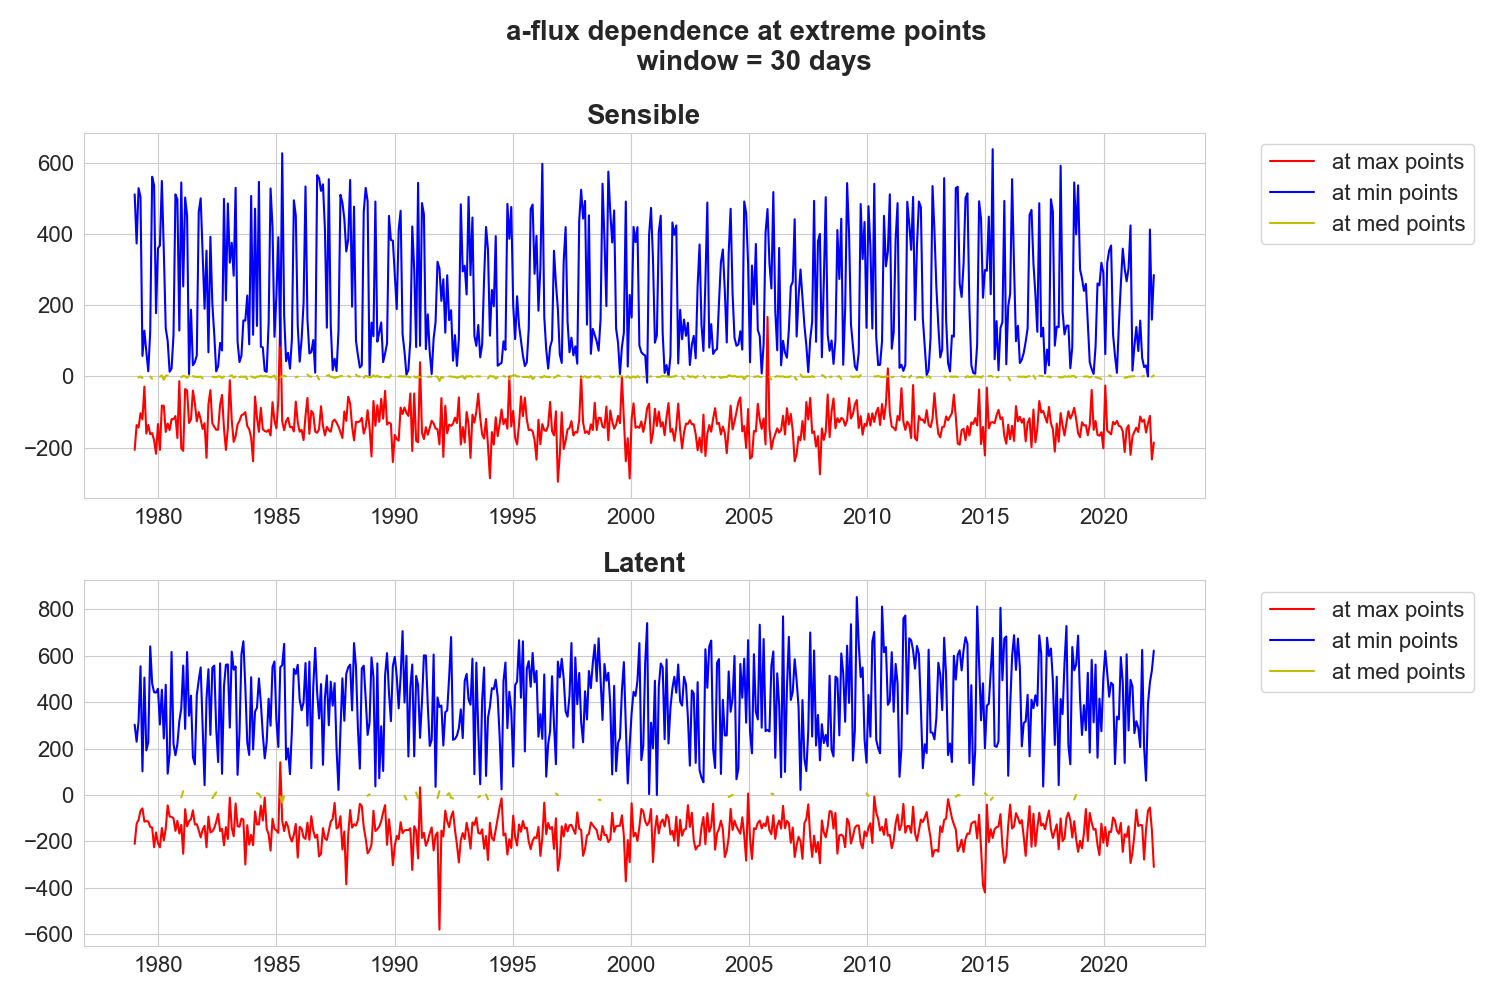
\includegraphics[width=\textwidth]{a_flux(1-15797)_30}
	\caption{Поведение оценок коэффициента $a$ в точках экстремальных значений потоков в течение $1979$--$2021$~гг. с шагом в $30$ дней}
	\label{fig:a_flux_month}
\end{figure}

\begin{figure}[!h]
	\centering
	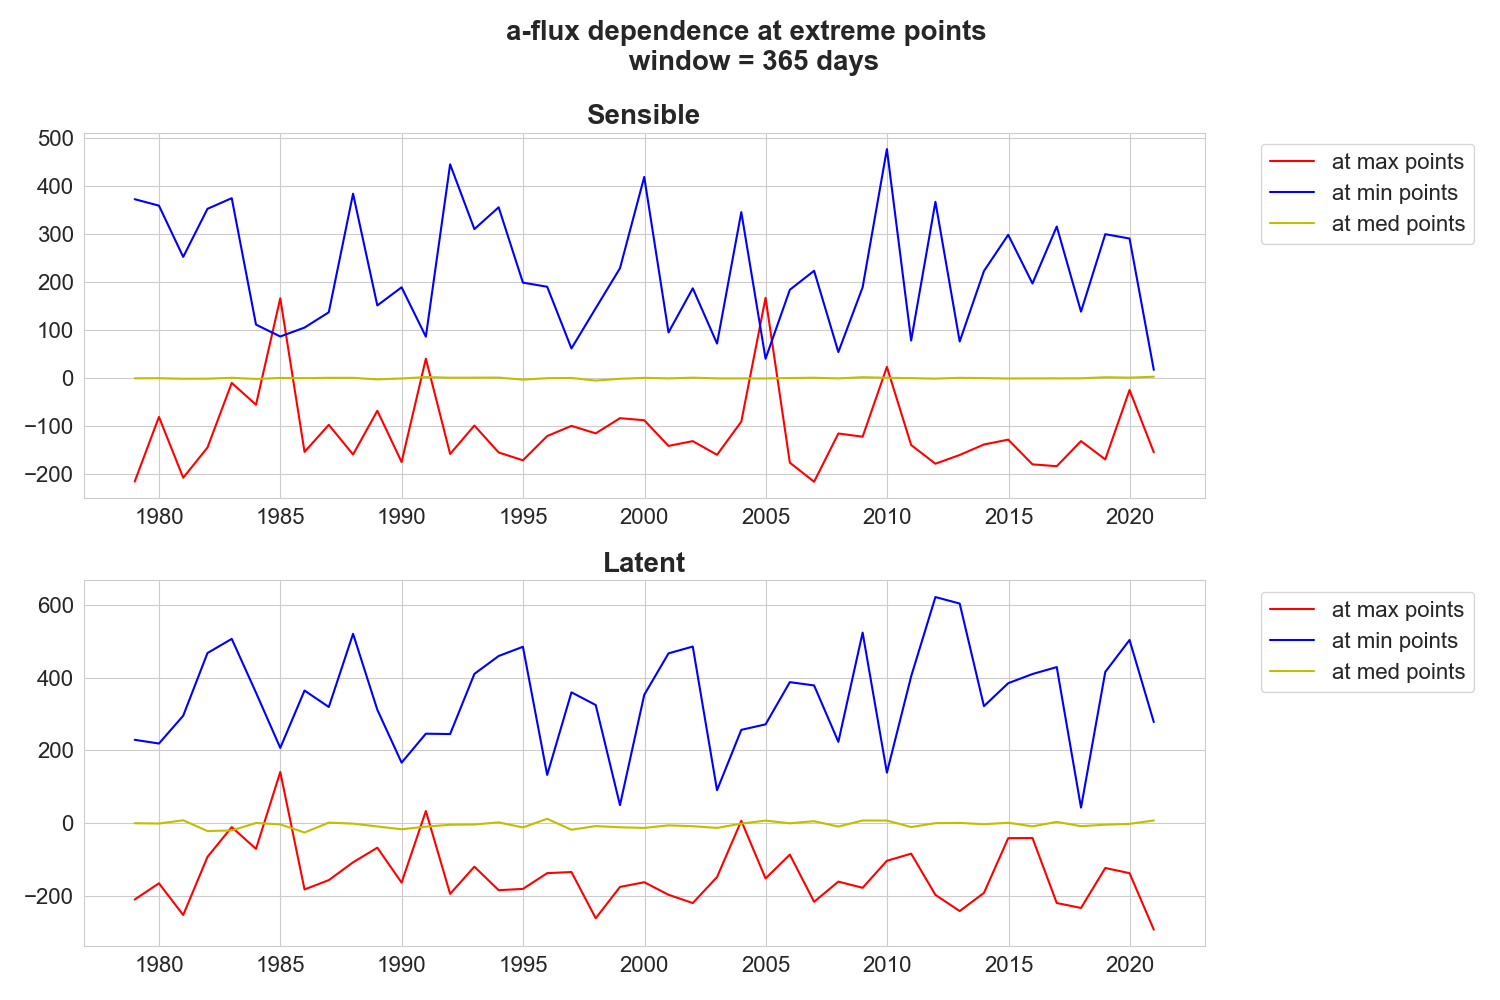
\includegraphics[width=\textwidth]{a_flux(1-15797)_365}
	\caption{Поведение оценок коэффициента $a$ в точках экстремальных значений потоков в течение $1979$--$2021$~гг. с шагом в $365$ дней}\label{fig:a_flux_year}
\end{figure}

\section{Разложение Карунена-Лоэва}
\label{sec:analysis}
В этом разделе представлены результаты применения методологии, описанной в разделе~\ref{sec:Karhunen}, к данным пространственно-временного реанализа ERA5. В данном разделе исследуется суммарный поток (сумма явных и скрытых тепловых потоков в каждой точке сетки), температура поверхности океана и атмосферное давление. В качестве средних значений они могут рассматриваться независимо в каждой точке.

\begin{figure}
	\centering
	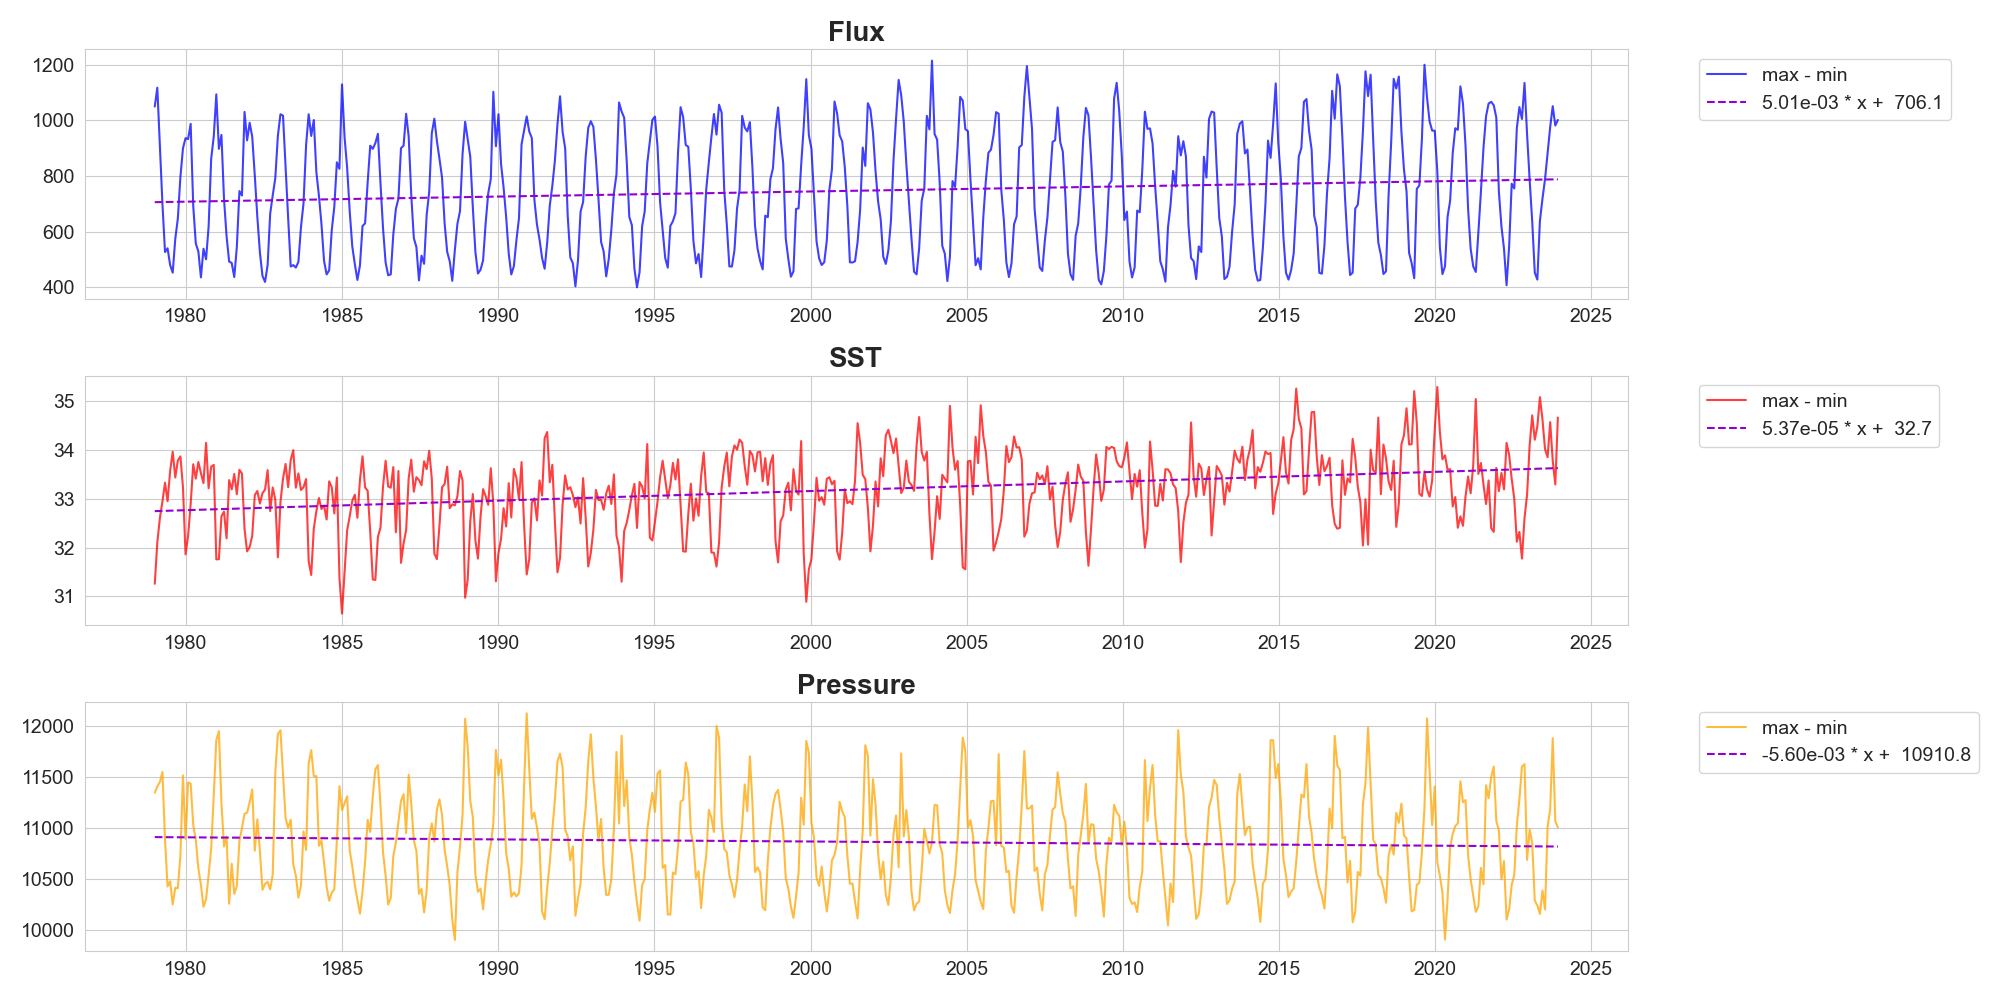
\includegraphics[width=1.0\textwidth]{difference_max-min_raw_(0-16554)_30.png}\\
	a)
	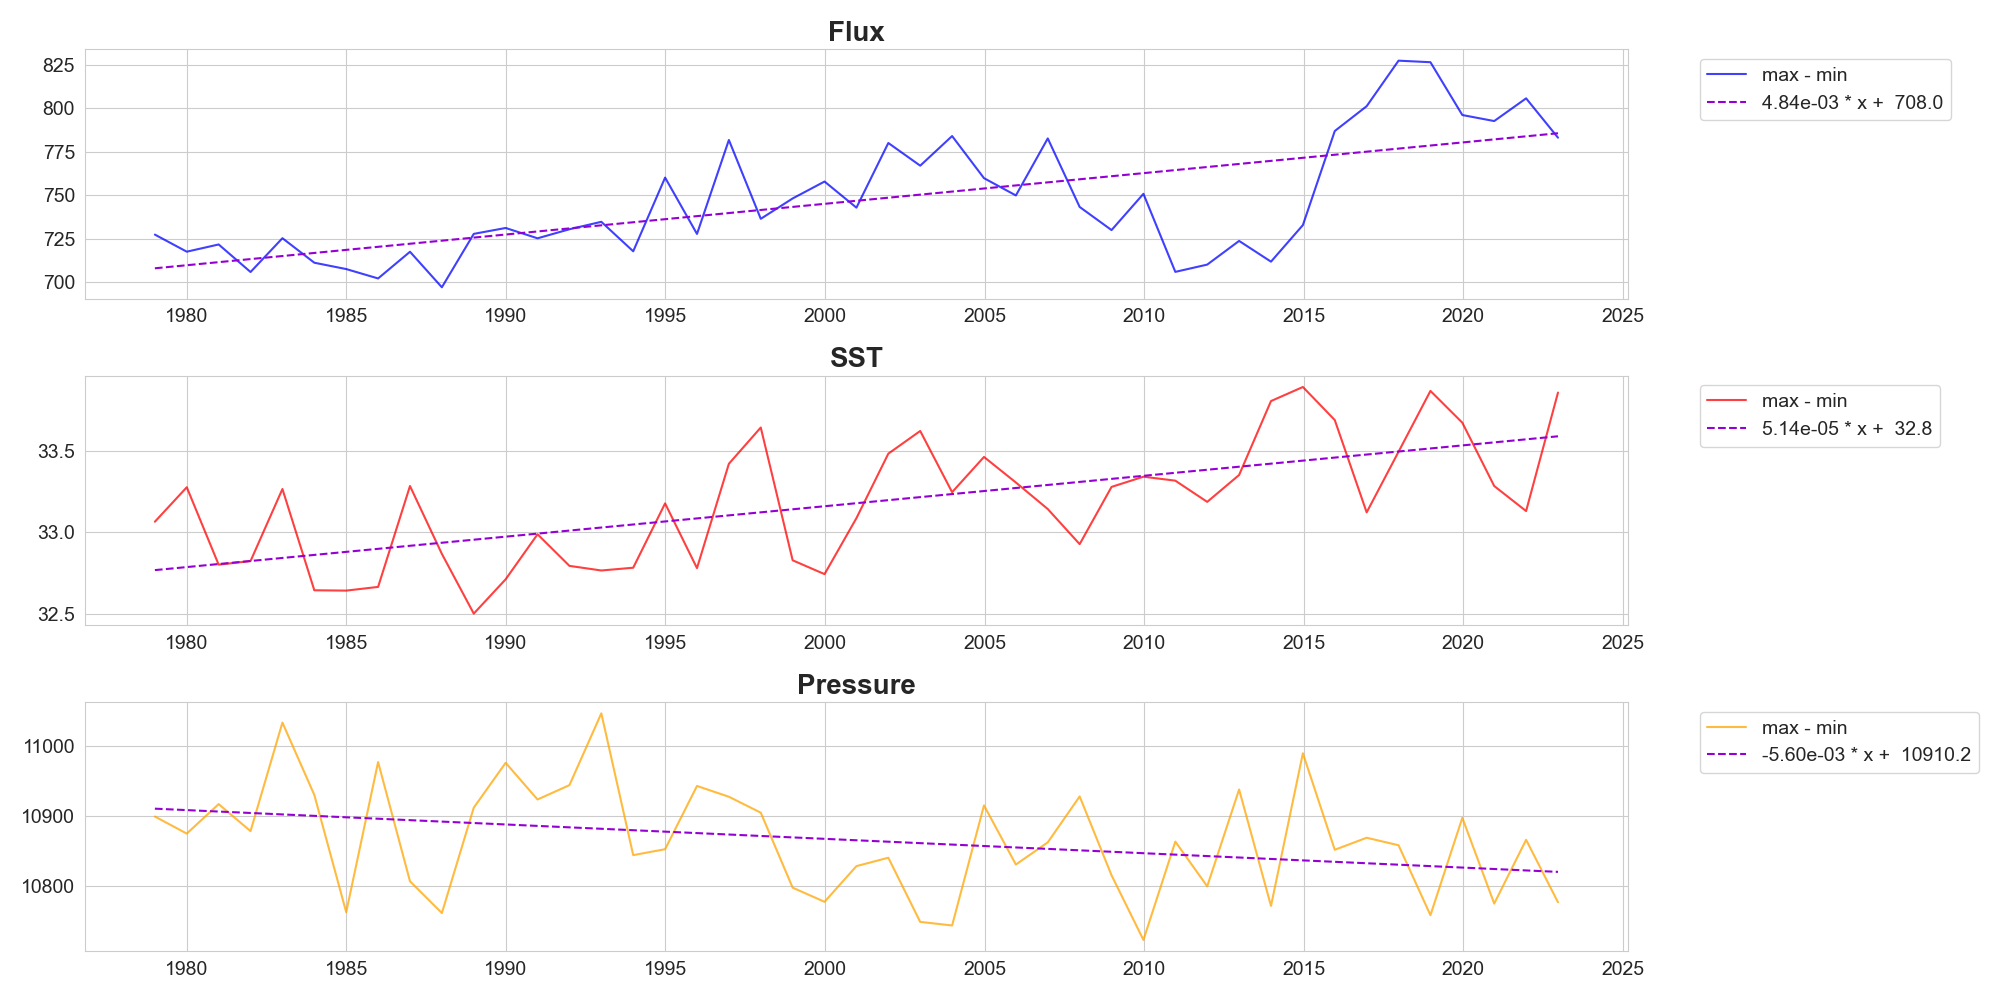
\includegraphics[width=1.0\textwidth]{difference_max-min_raw_(0-16554)_365.png}
	б)
	\caption{Разница между максимумом и минимумом по всей рассматриваемой области данных суммарного потока, SST и давления за $1979--2023$ годы при усреднении по окну шириной а) $30$ и б)$365$ дней}
	\label{fig:raw_trends}
\end{figure}

На рисунке~\ref{fig:a_extreme_365} представлены максимальное, среднее и минимальное значения построенных точечных оценок коэффициента $a$ по формуле~\eqref{eq:Ito} для временного ряда совокупного теплового потока, усредненного за годичный период. Хорошо виден ярко выраженный положительный линейный тренд для максимальных значений потока и SST (красная кривая) и незначительный значительный отрицательный тренд для минимальных значений (синяя кривая), причем для SST он выражен сильнее, чем для потоков. Средние значения не имеют выраженного тренда за весь рассматриваемый период (зеленая кривая). Также можно наблюдать почти двухлетний цикл, но он, по-видимому, не является статистически значимым. Длительные циклы слегка заметны, но не подтверждены. Для атмосферного давления тенденция прямо противоположная. Виден относительно сильный отрицательный тренд для максимальных значений и слабый положительный тренд для минимальных значений (красная и синяя кривые соответственно). Что касается SST, то для средних значений тренд вообще отсутствует (зеленая кривая).


\begin{figure}
	\centering
	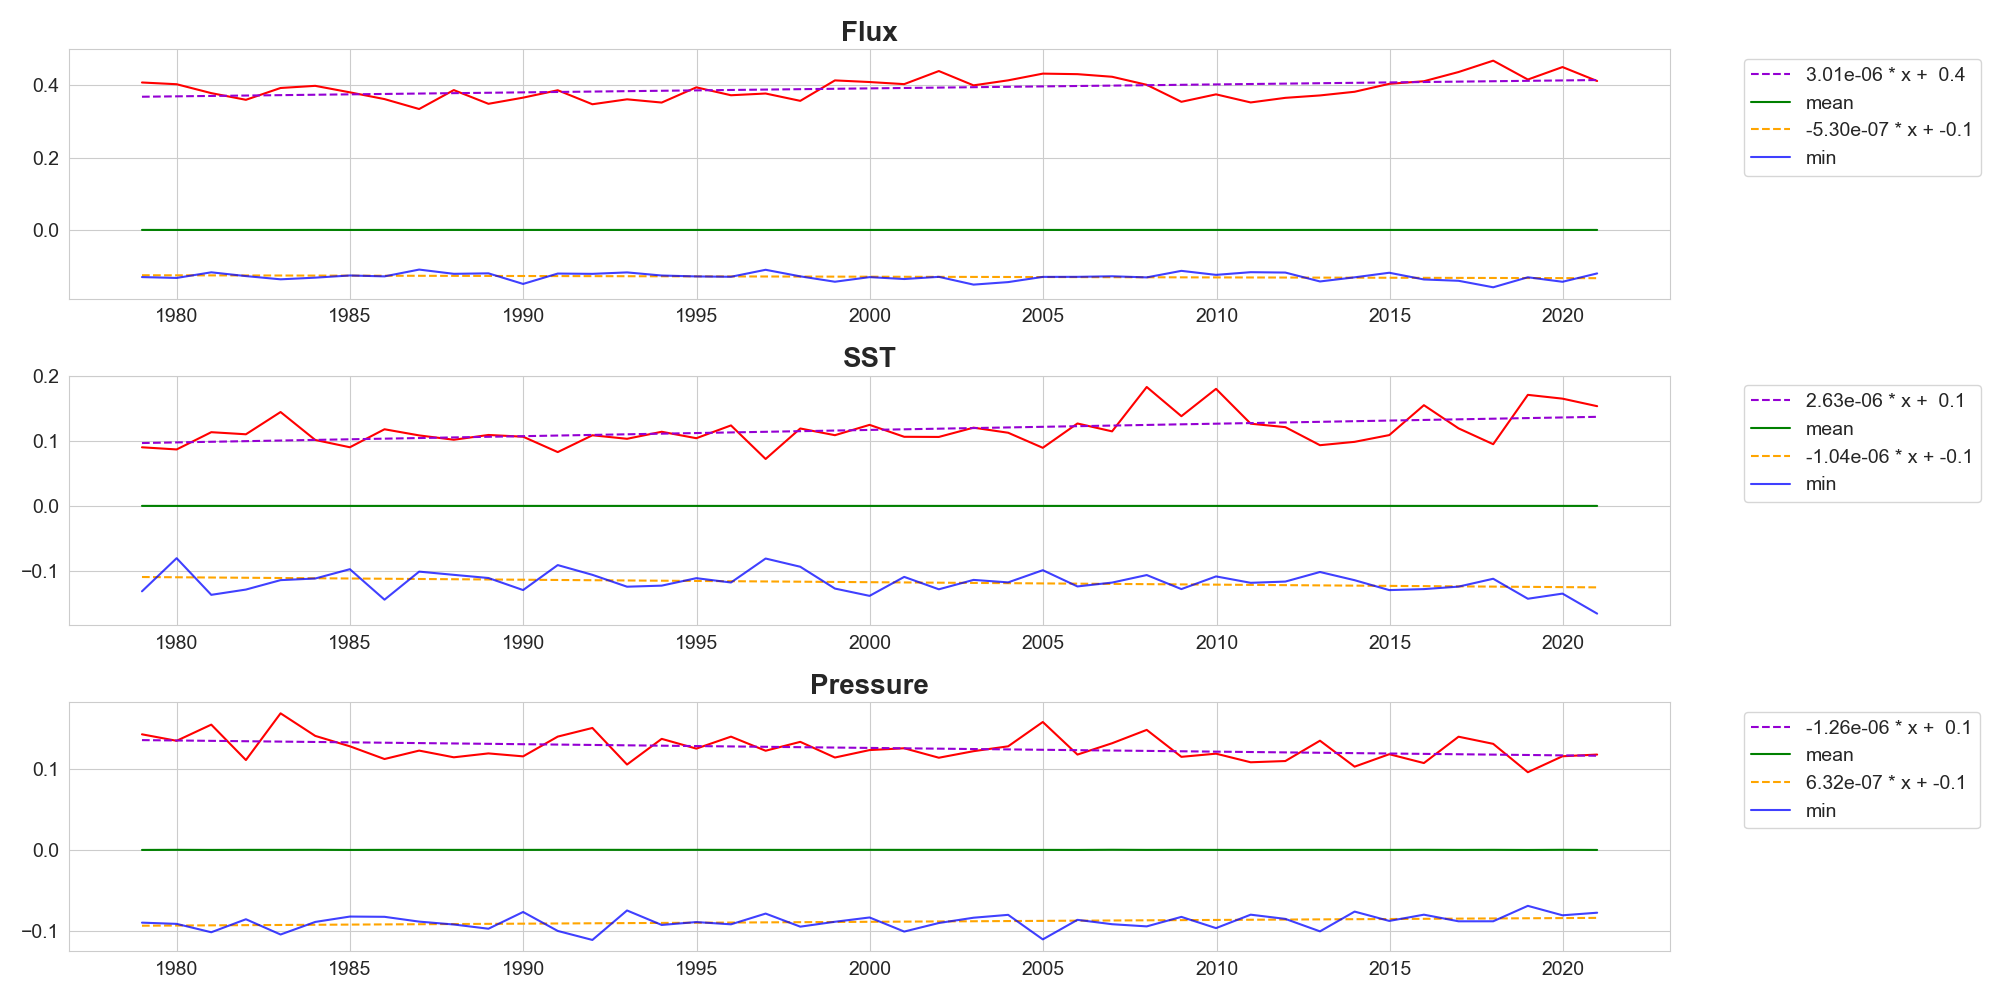
\includegraphics[width=1.0\textwidth]{a_(1-16071)_365_fit_regression.png}
	\caption{Динамика максимального, минимального и среднего значений оценок, полученных для коэффициента $a(X,t)$ для потока, SST и давления за период $1979-2024$ гг.} 
	\label{fig:a_extreme_365}
\end{figure}

В таблице~\ref{tab:angular_3d} представлены угловые коэффициенты для линейных трендов и приращения для максимальных и минимальных оценок коэффициентов дрейфа $A$ с ежемесячным и годовым усреднением.

\begin{table}
	\centering
	\begin{tabular}{|c|c|c|c|c|c|c|}
		\hline
		Переменная & Усреднение, дни & $k$ для максимума & прирост максимума & $k$ для минимума & прирост для минимума\\
		\hline
		Суммарный поток & $30$ & $2.86 \cdot 10^{-6}$ & $4.59 \cdot 10^{-2}$ & $-4.44 \cdot 10^{-7}$ & $-7.13 \cdot 10^{-3}$ \\
		Суммарный поток & $365$ & $3.01 \cdot 10^{-6}$ & $4.85 \cdot 10^{-2}$ & $-5.30 \cdot 10^{-7}$ & $-8.52 \cdot 10^{-3}$    \\
		SST & $30$ & $2.71 \cdot 10^{-6}$ & $4.35 \cdot 10^{-2}$ & $-1.21 \cdot 10^{-6}$ & $-1.95 \cdot 10^{-2}$   \\
		SST & $365$ & $2.63 \cdot 10^{-6}$ & $4.23 \cdot 10^{-2}$ & $-1.04 \cdot 10^{-6}$ & $-1.67 \cdot 10^{-2}$    \\
		Давление & $30$ & $-1.30 \cdot 10^{-6}$ & $-2.10 \cdot 10^{-2}$ & $7.29 \cdot 10^{-7}$ & $1.17 \cdot 10^{-2}$ \\
		Давление & $365$ & $-1.26 \cdot 10^{-6}$ & $-2.03 \cdot 10^{-2}$ & $6.32 \cdot 10^{-7}$ & $1.01 \cdot 10^{-2}$ \\
		\hline
	\end{tabular}
	\caption{Угловые коэффициенты линейного тренда для максимальной и минимальной оценок коэффициента сноса $a$ с различными масштабами усреднения}
	\label{tab:angular_3d}
\end{table}


На рисунках ~\ref{fig:SST-SST_trends}--~\ref{fig:Flux-SST_trends} показана эволюция экстремальных характеристик (максимума, минимума и среднего значения) для первого собственного вектора из упорядоченного набора для пар SST-SST и Flux-SST, соответственно, и соответствующие линии линейной регрессии, где переменной Flux обозначается суммарный тепловой поток, а упорядочивание происходит по убыванию модулей соответствующих собственных значений. Для всех этих временных рядов практически нет тренда, поскольку угловые коэффициенты оценочной регрессии имеют порядок от $10^{-8}$ до $10^{-6}$ и кажутся слишком малыми по сравнению с масштабом ряда, чтобы считаться значимыми. Следует отметить, что для минимальных значений SST наблюдается заметно больший диапазон колебаний от года к году. Для пары Flux-Flux картина аналогична паре SST-SST, но амплитуда годового хода значительно меньше.

\begin{figure}
	\centering
	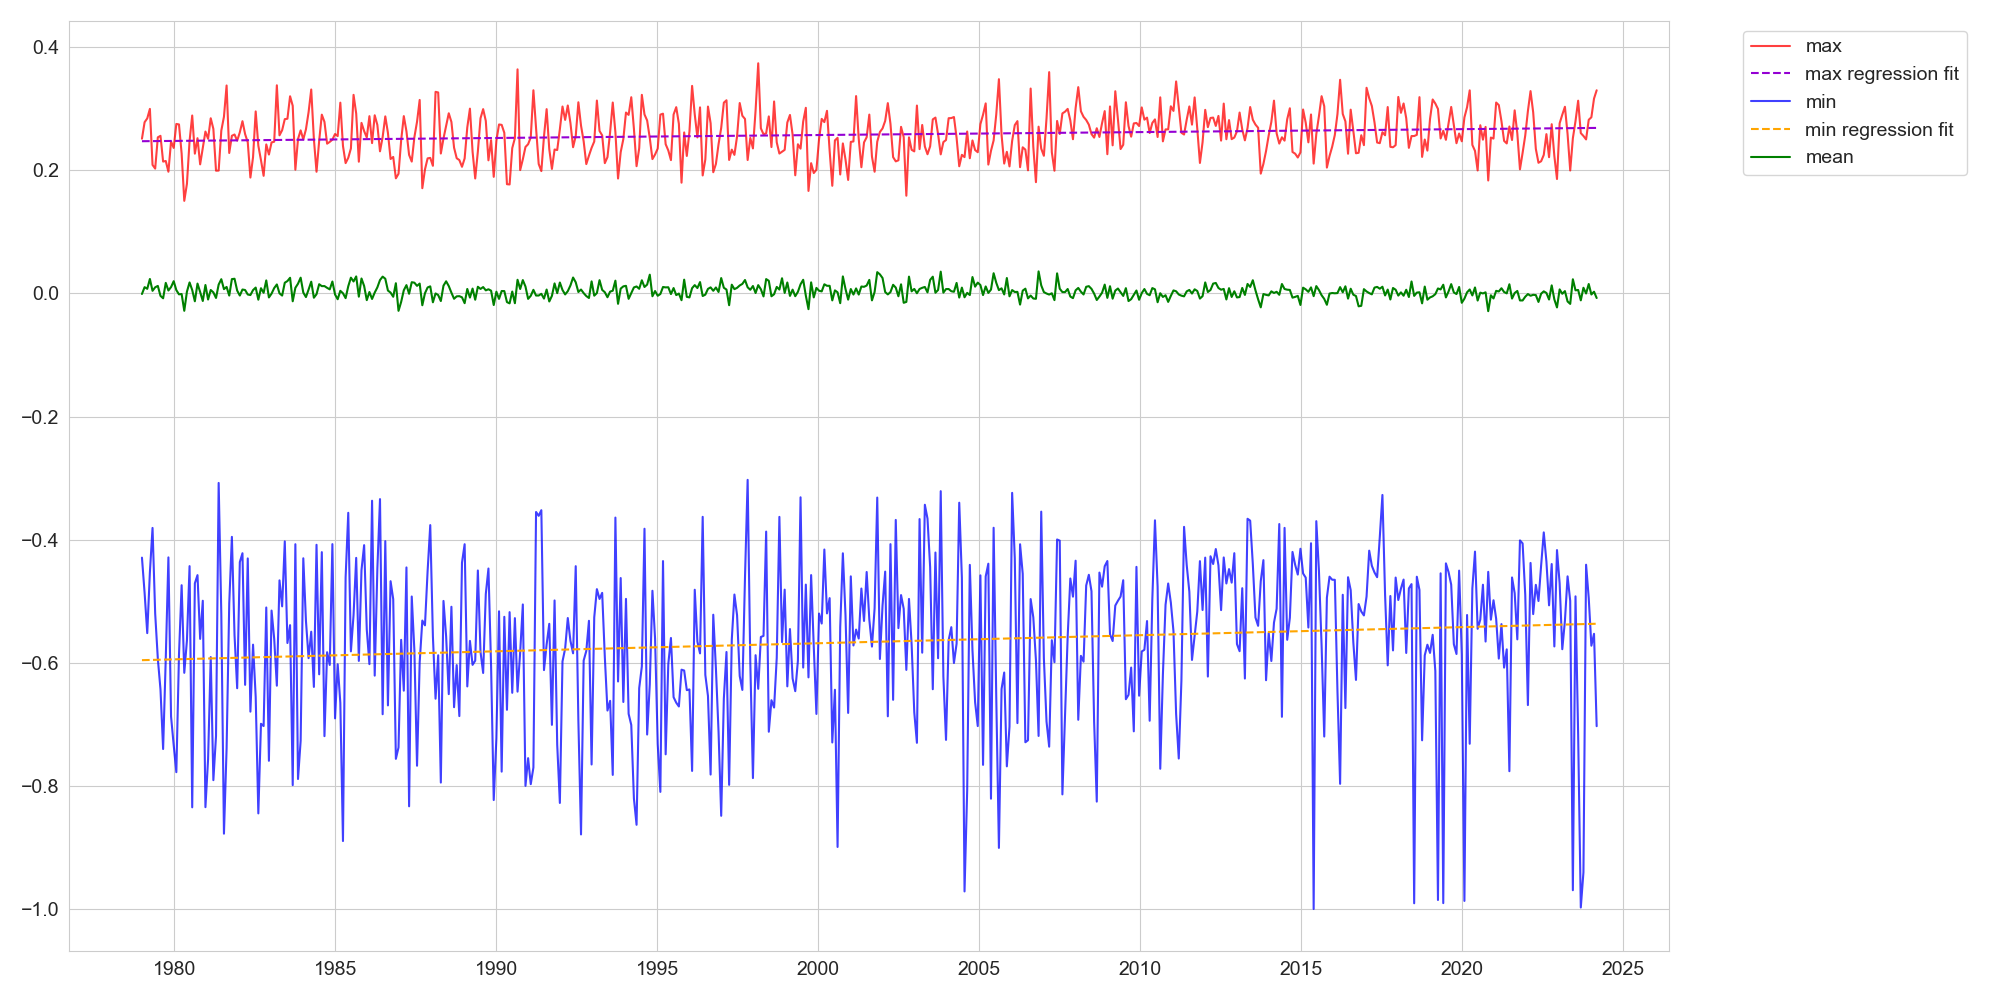
\includegraphics[width=1.0\textwidth]{SST-SST_(0-16554)_mean_30_fit_regression.png}
	\caption{Экстремальные значения и их тренды для первого собственного значения из упорядоченного набора для пары SST-SST за $1979--2024$ годы с усреднением в $30$ дней}
	\label{fig:SST-SST_trends}
\end{figure}

\begin{figure}
	\centering
	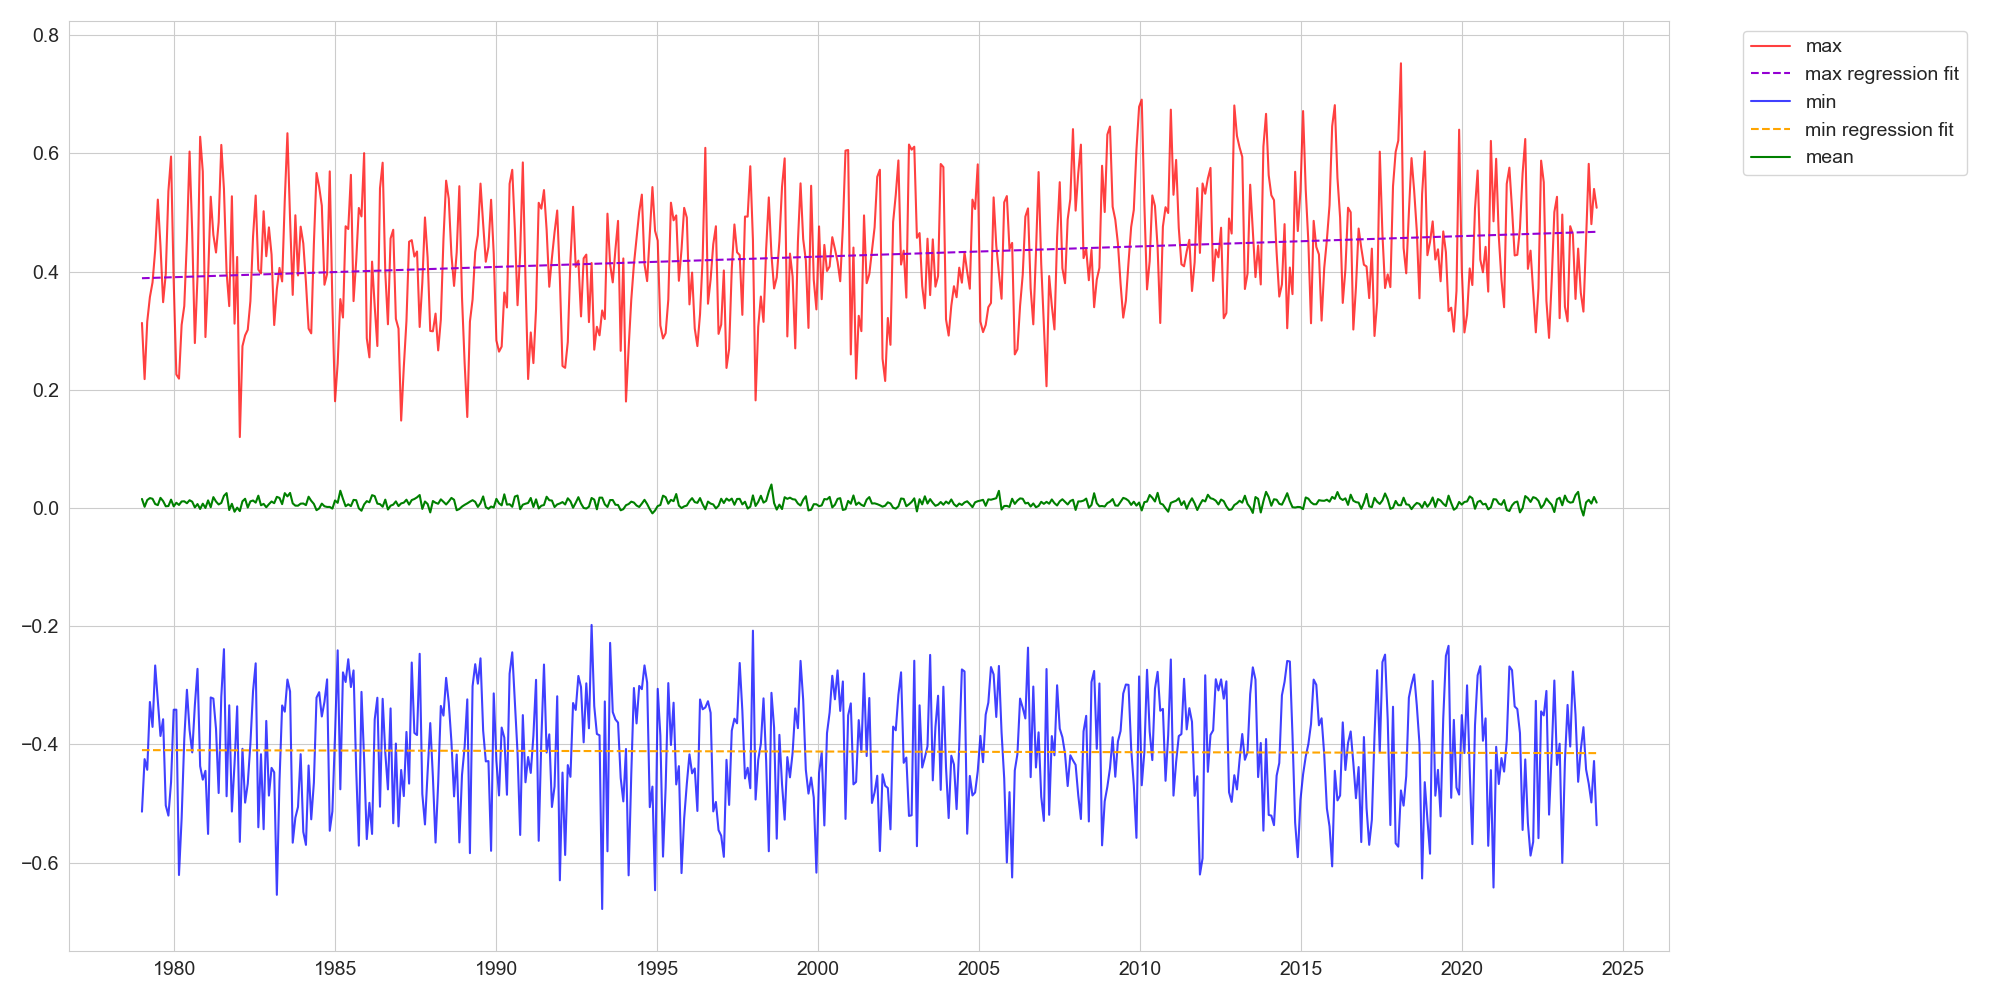
\includegraphics[width=1.0\textwidth]{Flux-SST_(0-16554)_mean_30_fit_regression.png}
	\caption{Экстремальные значения и их тренды для первого собственного значения из упорядоченного набора для пары Flux-SST за $1979--2024$ годы с усреднением в $30$ дней}
	\label{fig:Flux-SST_trends}
\end{figure}

На рисунке~\ref{fig:Flux-Flux_eigenvectors} хорошо виден волновой и динамический перенос тепла вдоль атлантической меридиональной циркуляционной системы. Волна жары, фронт которой проходит от побережья Северной Америки до Африки, двигаясь с юга на север, захватывается системой течений вдоль Атлантического побережья (Гольфстрим и Североатлантическое течение) и затухает в северо-восточном направлении.

С помощью этих данных можно количественно оценить энергию волны и скорость ее рассеяния. Следующие два собственных вектора из упорядоченного набора имеют значения, близкие друг к другу, и на $10$ порядков меньше, чем первый собственный вектор. Структуры этих векторов похожи друг на друга и, как правило, повторяют первый собственный вектор. При визуализации собственных векторов используется цветовая шкала, аналогичная SST и давлению, показанным на рисунке ~\ref{fig:data_example}: цвет меняется с белого при значениях, близких к нулю, а затем на темно-синий при увеличении значений. Яркость цвета в определенной точке соответствует расстоянию значения от нуля. Светло-зеленый цветом показаны участки суши.

Собственные векторы матрицы SST (см. рисунок ~\ref{fig:SST-SST_eigenvectors}) аналогичны собственным векторам матрицы Flux, но имеют заметные отличия. Перенос тепла с юга на север происходит в основном в виде крупномасштабных вихрей, которые перемещаются вдоль системы течений и ослабевают в районах Исландского минимума и к югу от Азорских островов. Здесь различия первого собственного вектора в терминах собственных значений имеют тот же порядок, что и для SST, однако структурно второй и третий собственные векторы, по-видимому, отстают по отношению к основному собственному вектору. Также можно оценить общую энергию этих потоков как сумму квадратов собственных значений матрицы диффузии.


Пара давление-давление (см. рисунок~\ref{fig:press-press_eigenvectors}) демонстрирует создание и динамику крупномасштабных структур в Северной Атлантике. Кольца давления проходят через весь Атлантический регион, в основном концентрируясь в северной части вблизи Исландской минимальной зоны и энергетической зоны Лабрадора. Для первого сильно доминирующего собственного вектора динамика в основном наблюдается вдоль Гольфстрима в направлении Североатлантической Исландской минимальной зоны, но для второго и третьего собственных векторов (которые значительно меньше по абсолютным значениям) мы наблюдаем более сложную динамику.

\begin{table}
	\caption{Угловые коэффициенты линейного тренда для собственных значений с различными масштабами усреднения }
	\centering
	\begin{tabular}{|c|c|c|}
		\hline
		Пара & $k$ для усреднения в $30$ дней & $k$ для усреднения в $365$ дней\\
		\hline
		Flux-Flux & $-1.87 \cdot 10^{4}$ & $-5.26 \cdot 10^{3}$ \\
		SST-SST & $1.32 \cdot 10^{1}$ & $1.31 \cdot 10^{1}$ \\
		Давление-давление & $1.31 \cdot 10^{6}$ & $1.73 \cdot 10^{6}$ \\
		Flux-SST & $2.95 \cdot 10^{2}$ & $2.96 \cdot 10^{2}$ \\
		SST-давление & $2.34 \cdot 10^{3}$ & $2.33 \cdot 10^{3}$ \\
		Flux-давление & $-2.10 \cdot 10^{4}$ & $3.59 \cdot 10^{4}$ \\
		\hline
	\end{tabular}
	\label{tab:angular_eigens}
\end{table}

На рисунках~\ref{fig:eigenvalues_mean_30} и ~\ref{fig:eigenvalues_mean_365} показана эволюция первых собственных значений из упорядоченного набора (отсортированных по убыванию их абсолютных значений) с усреднением по окну шириной в $30$ и $365$ дней, соответственно, а также соответствующие линейные тренды. Таблица~\ref{tab:angular_eigens} показывает угловые коэффициенты трендов для обоих масштабов усреднения.


\begin{figure}
	\centering
	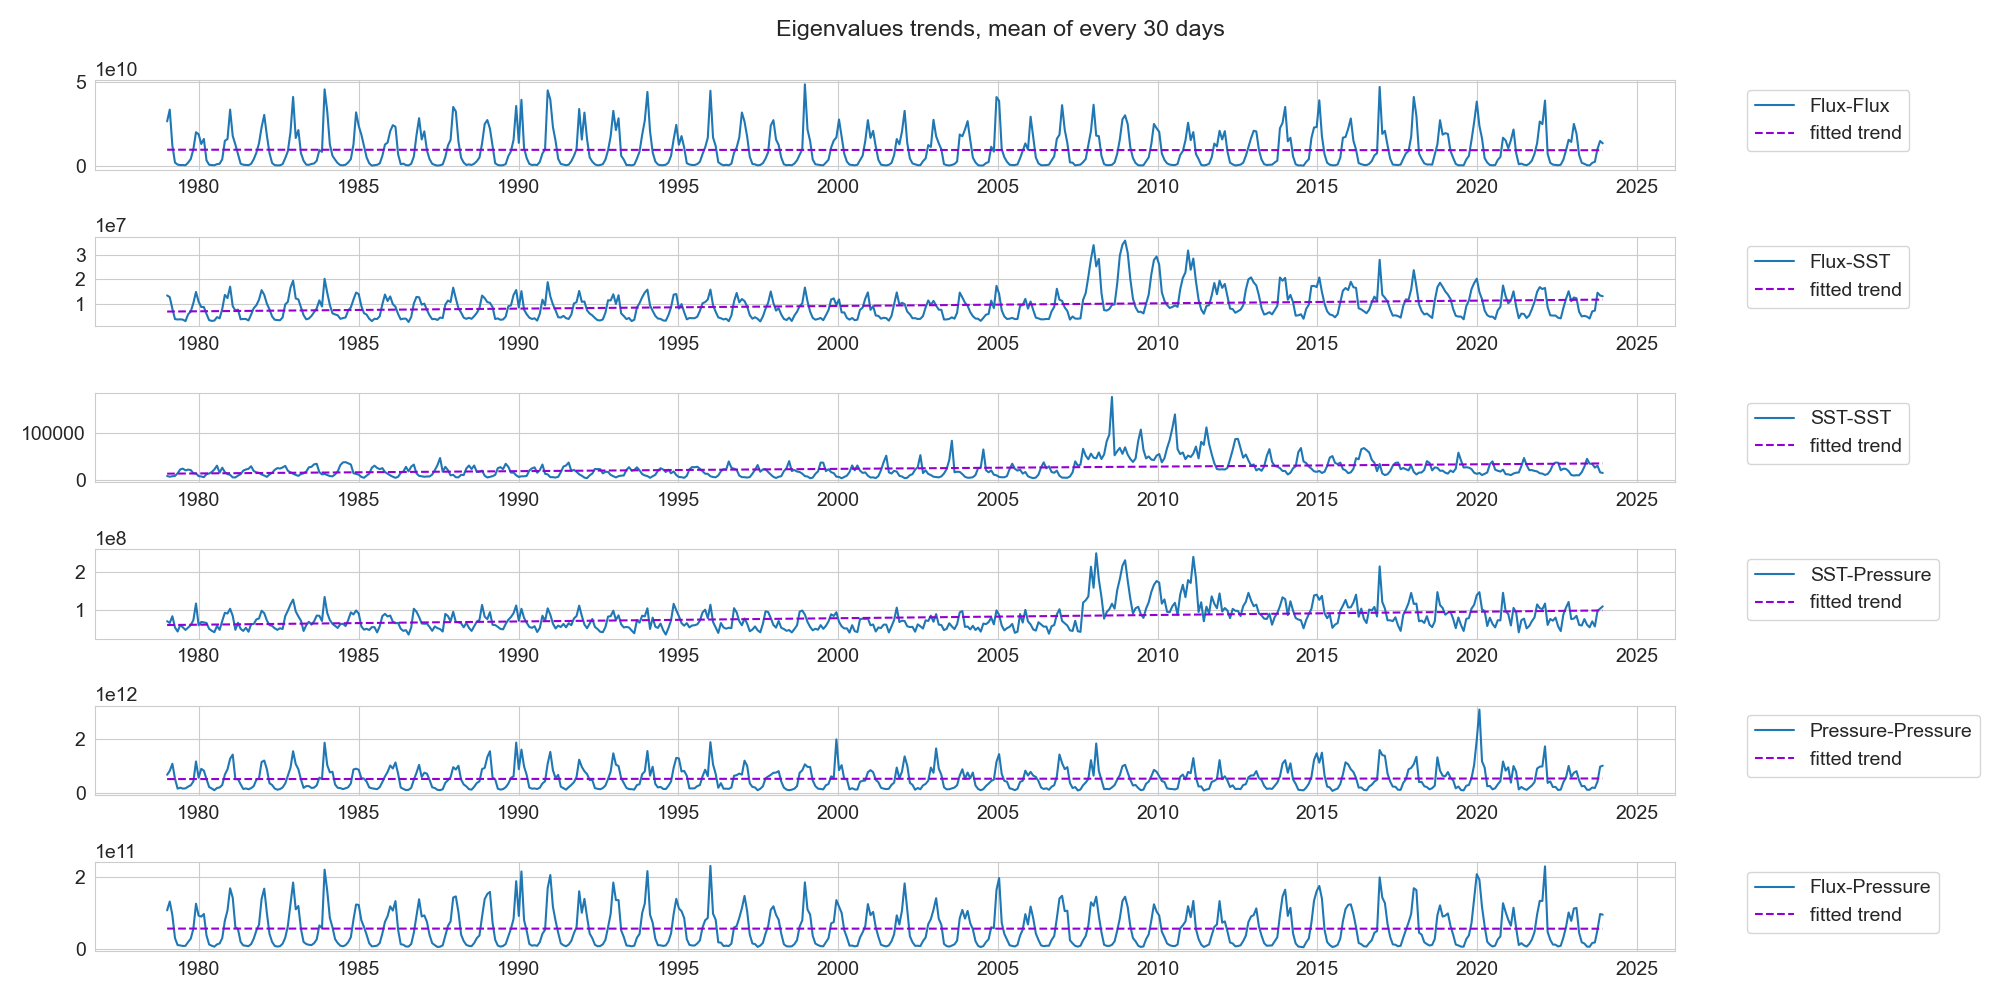
\includegraphics[width=\textwidth]{(0-16767)_mean_30_fit_regression_eigenvalues.png}
	\caption{Первые собственные значения упорядоченного набора для каждой пары переменных, усредненные за $30$ дней и их линейные тренды}
	\label{fig:eigenvalues_mean_30}
\end{figure}

\begin{figure}
	\centering
	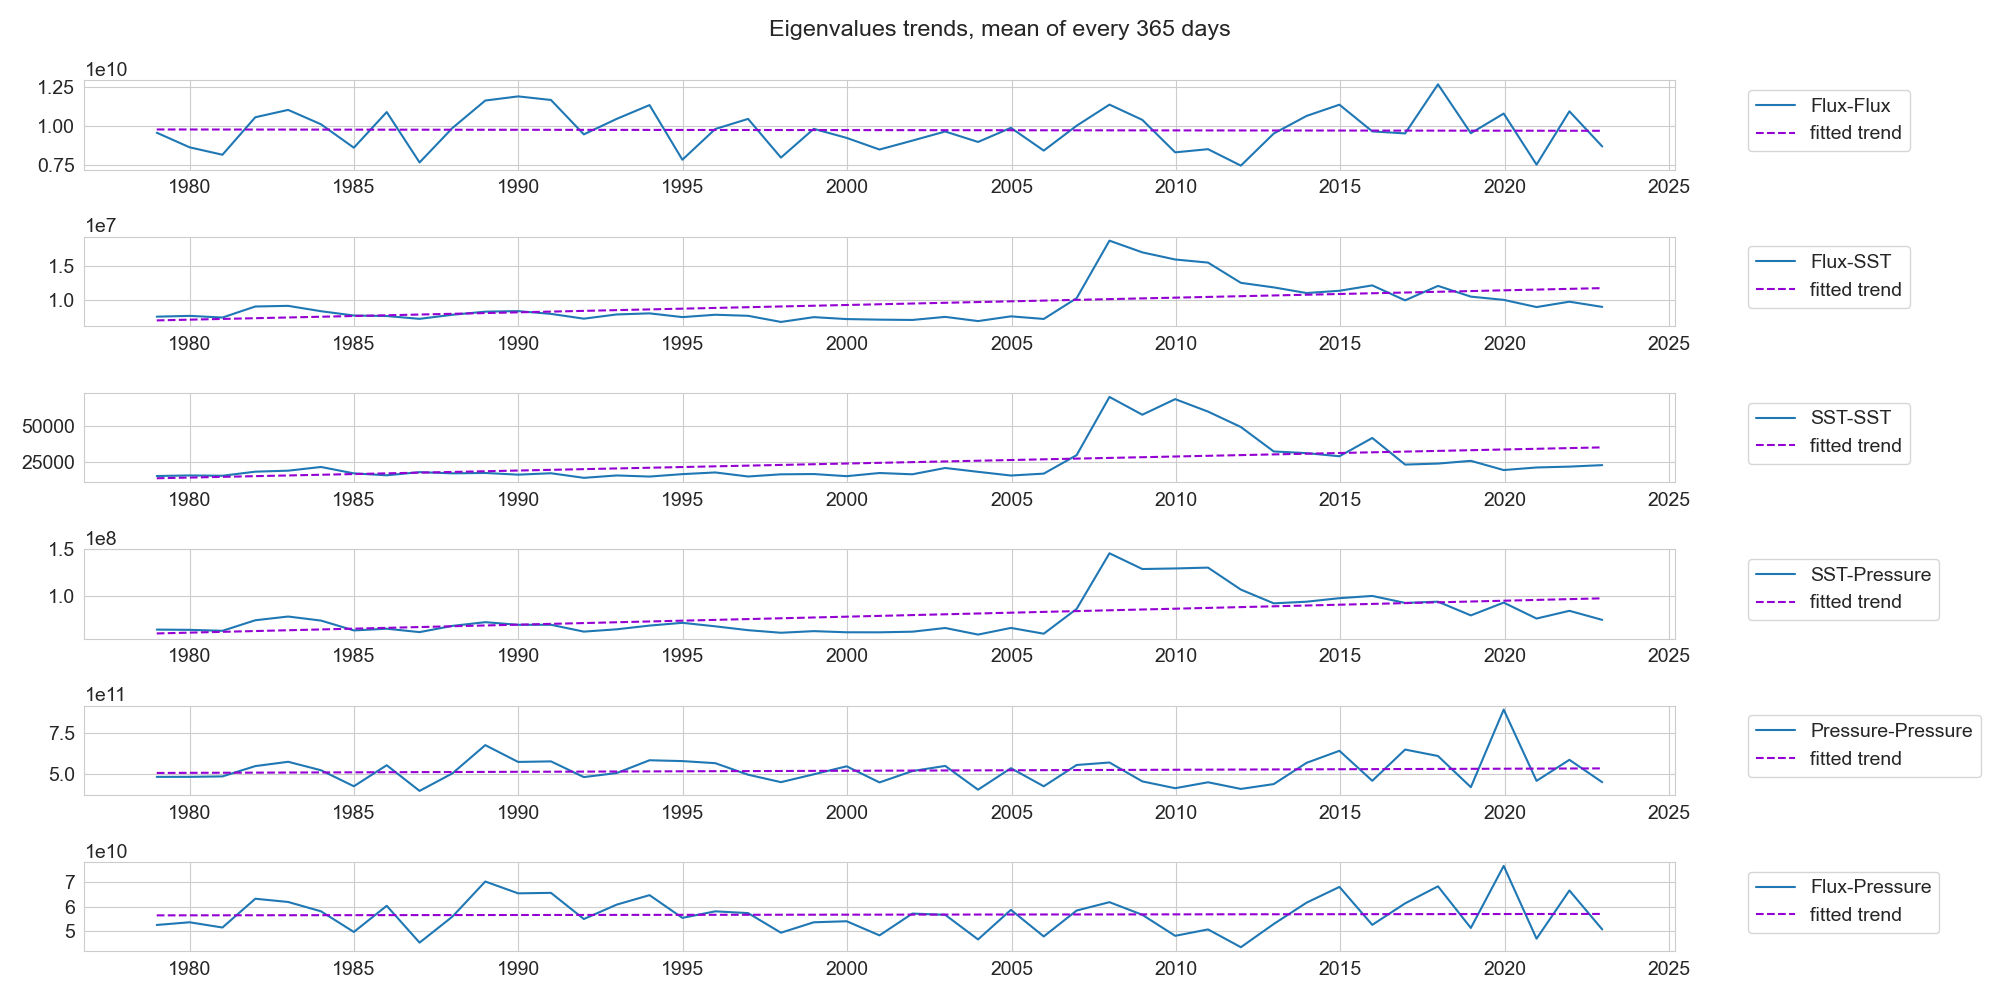
\includegraphics[width=\textwidth]{(0-16767)_mean_365_fit_regression_eigenvalues.png}
	\caption{Первые собственные значения упорядоченного набора для каждой пары переменных, усредненные за $365$ дней и их линейные тренды}
	\label{fig:eigenvalues_mean_365}
\end{figure}

\begin{figure}
	\centering
	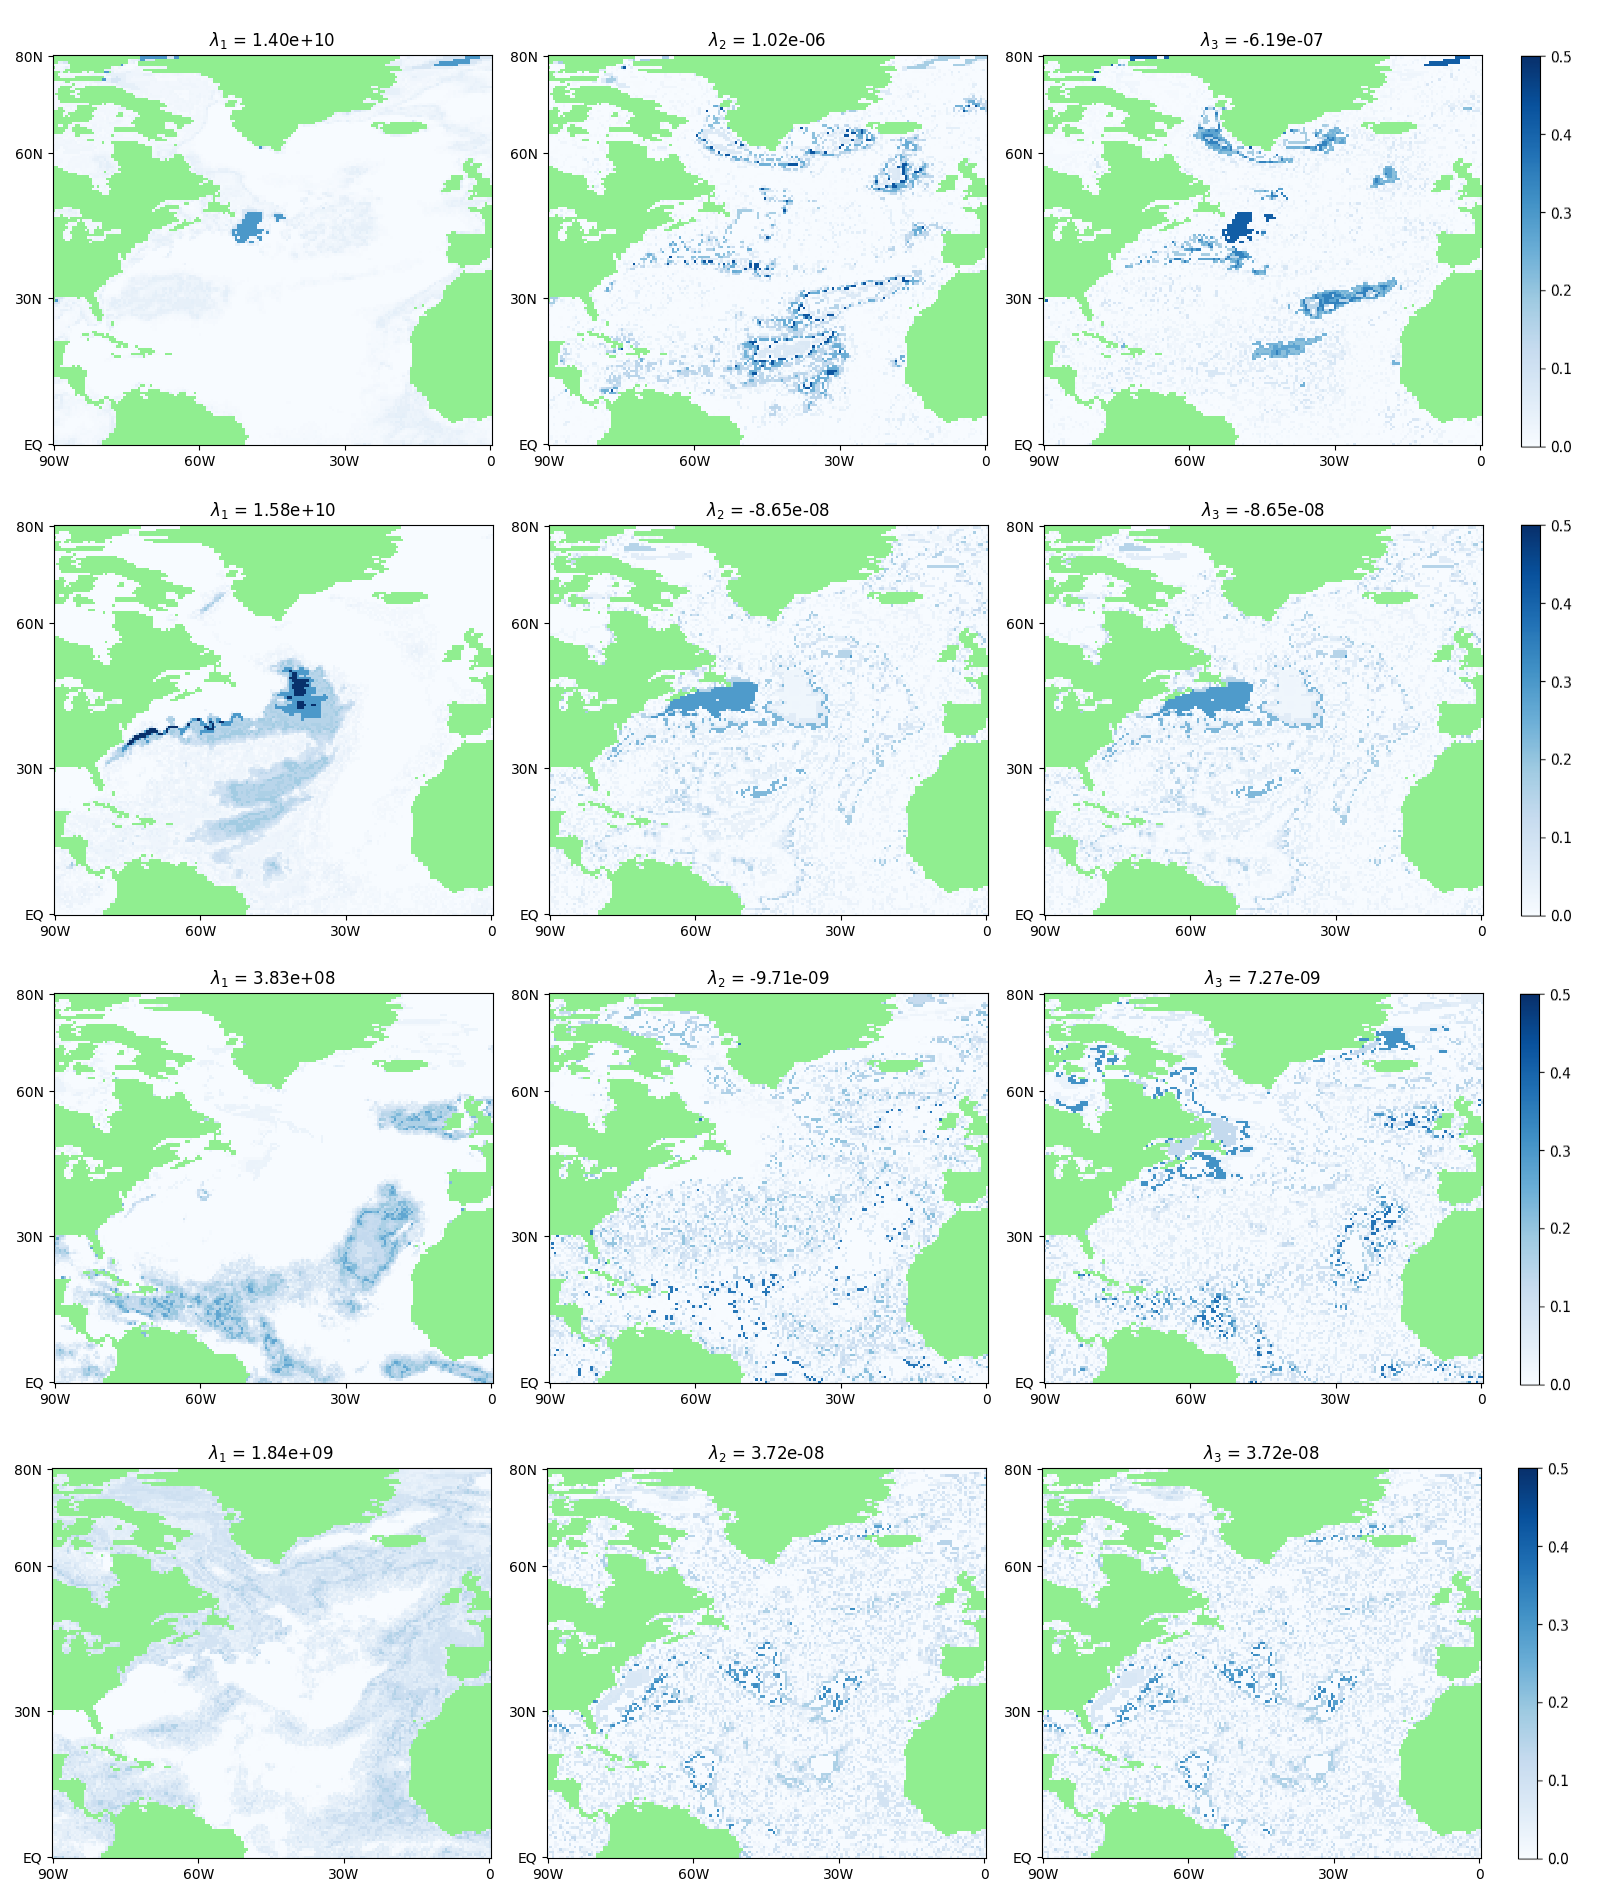
\includegraphics[width=\textwidth]{flux-flux_eigenvectors.png}
	\caption{Первые три собственных вектора из упорядоченного набора для пары Поток-поток за $01.01.23$, $01.04.23$, $01.07.23$ и $01.10.23$}
	\label{fig:Flux-Flux_eigenvectors}
\end{figure}

\begin{figure}
	\centering
	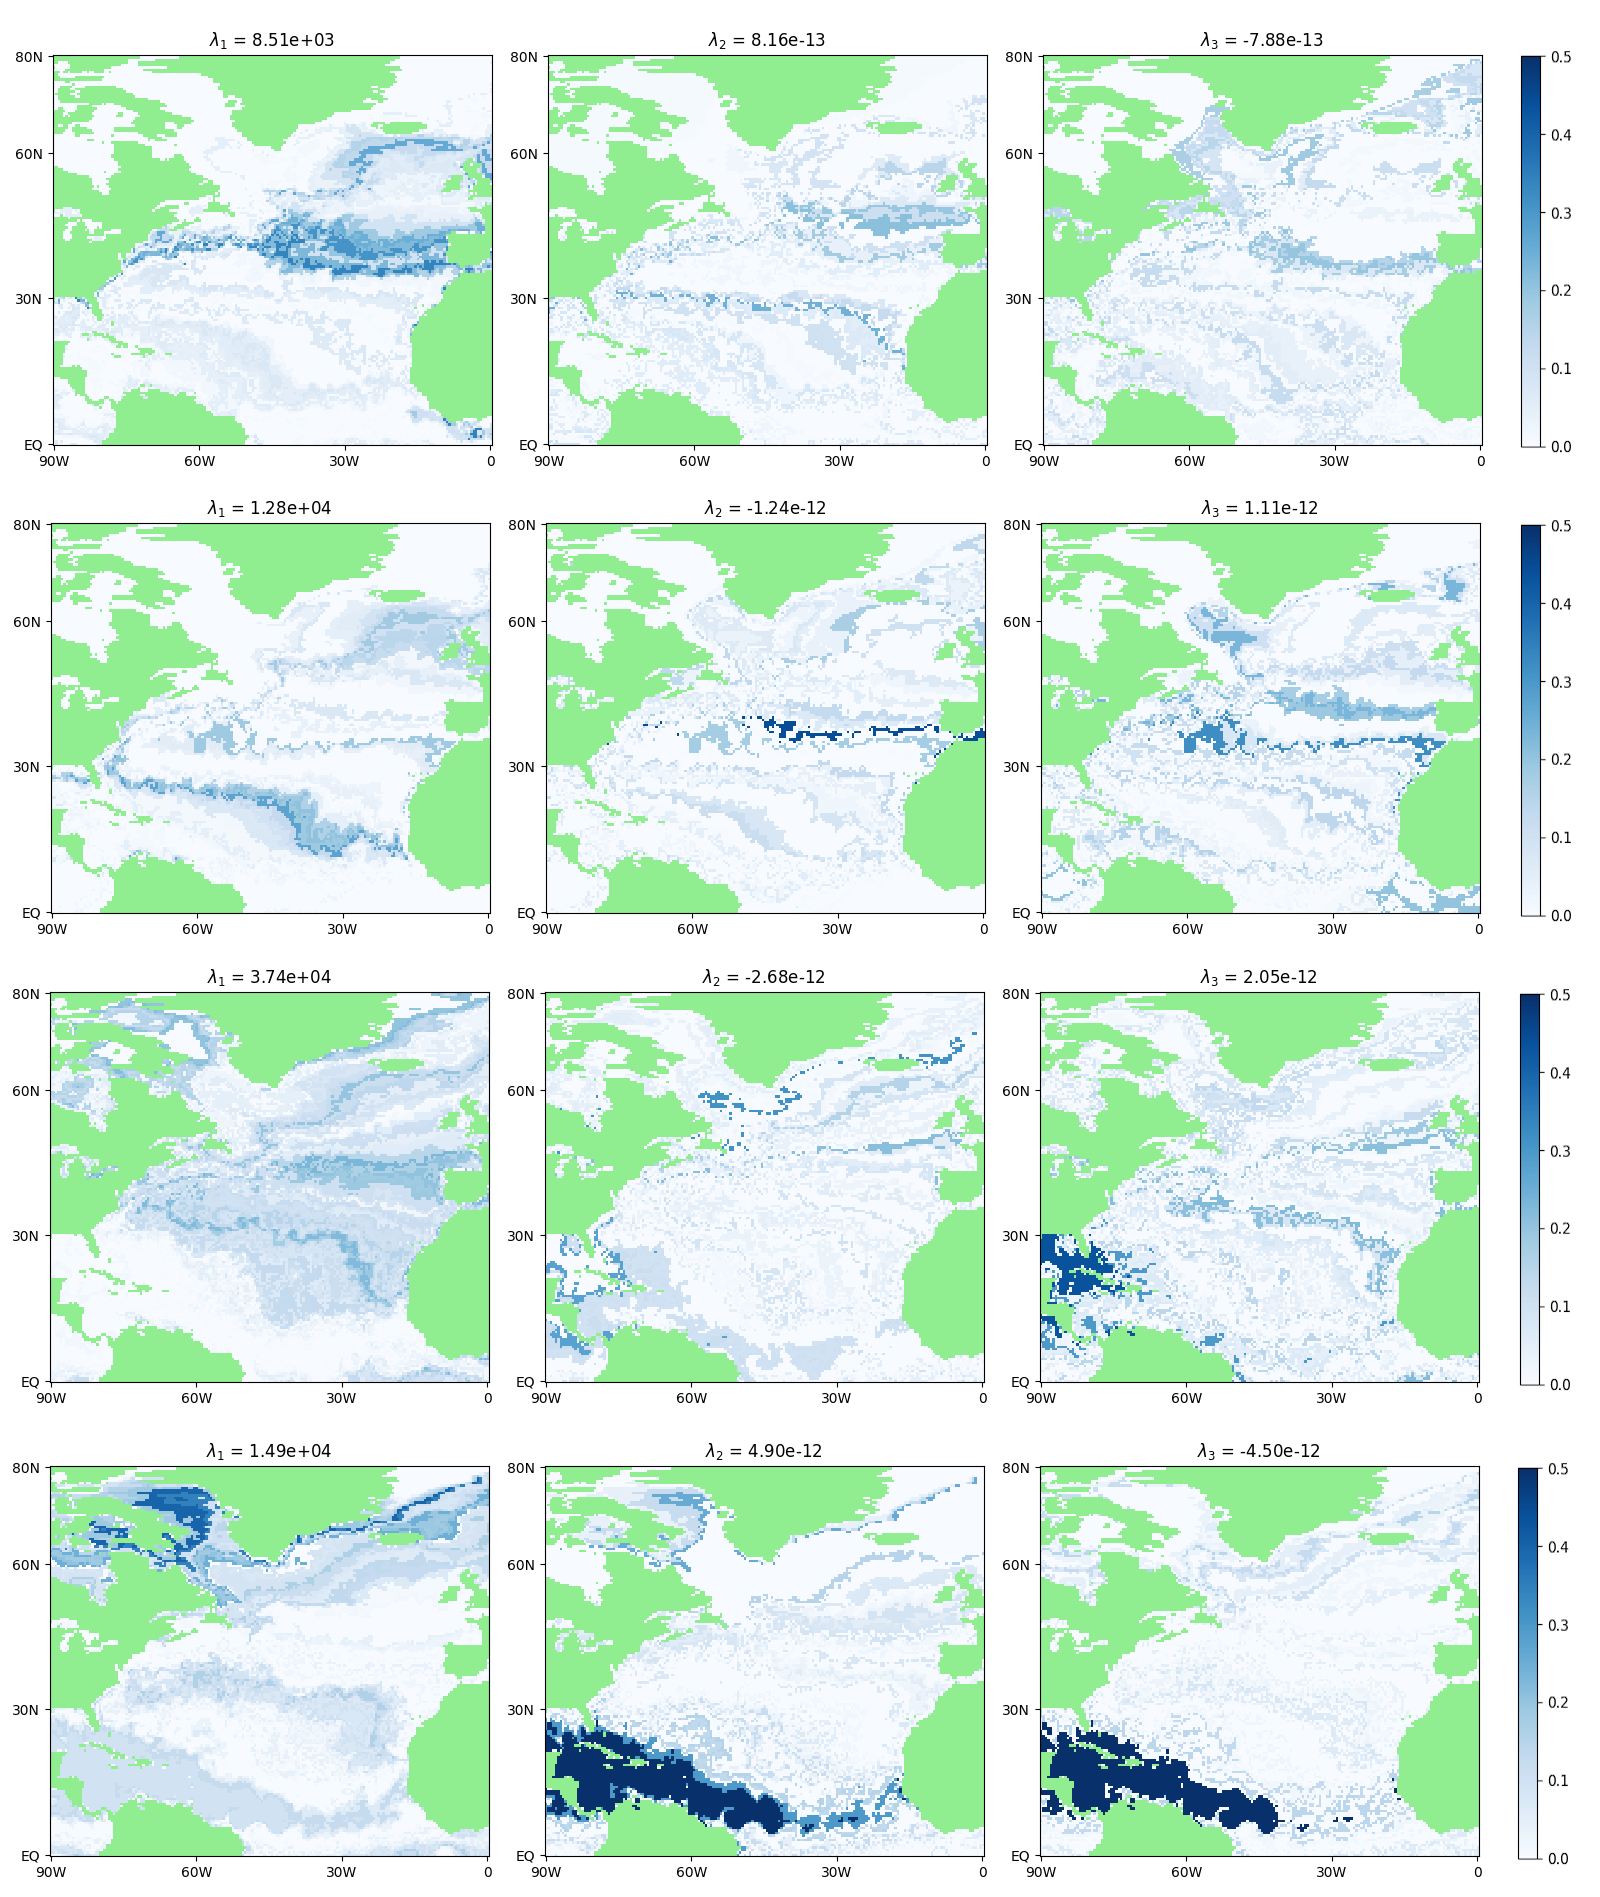
\includegraphics[width=\textwidth]{sst-sst_eigenvectors.png}
	\caption{Первые три собственных вектора из упорядоченного набора для пары SST-SST за $01.01.23$, $01.04.23$, $01.07.23$ и $01.10.23$}
	\label{fig:SST-SST_eigenvectors}
\end{figure}

\begin{figure}
	\centering
	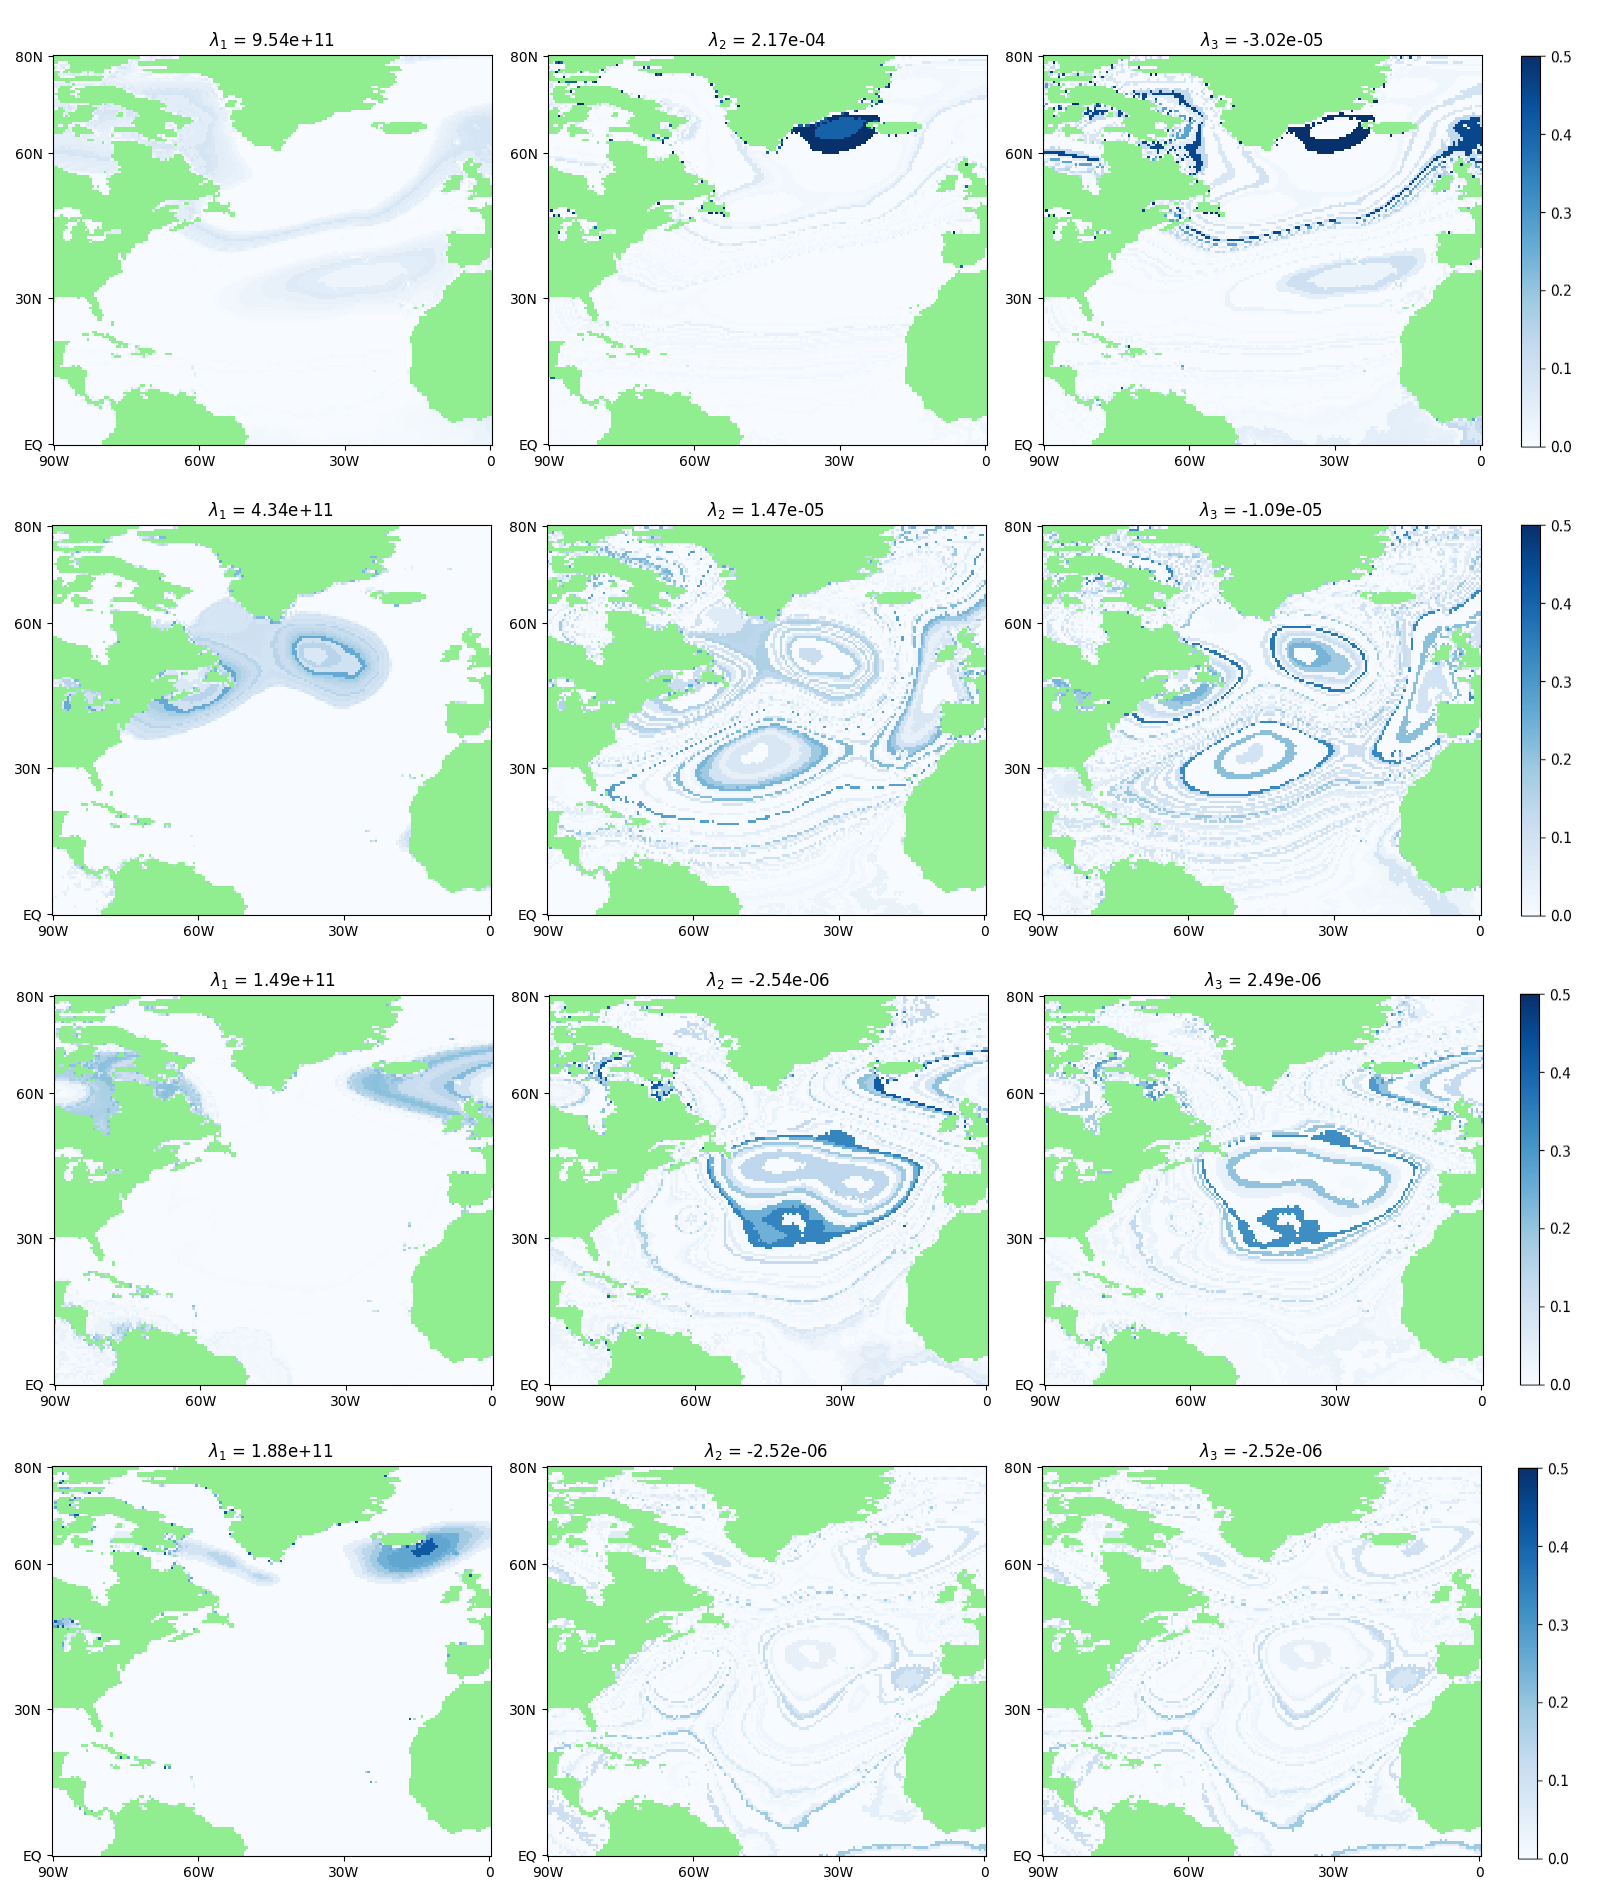
\includegraphics[width=\textwidth]{press-press_eigenvectors.png}
	\caption{Первые три собственных вектора из упорядоченного набора для пары Давление-Давление за $01.01.23$, $01.04.23$, $01.07.23$ и $01.10.23$}
	\label{fig:press-press_eigenvectors}
\end{figure}

\section{Взаимосвязь между потоком, SST и давлением}
В этом разделе рассматривается взаимосвязь между суммарным тепловым потоком (суммой явных и скрытых тепловых потоков в каждой точке сетки), температурой поверхности океана и атмосферным давлением с помощью их совместных диффузионных матриц. В статье~\cite{gorshenin2023stochastic} была рассмотрена временная изменчивость явных и скрытых тепловых потоков за практически тот же временной период. Построение совместных матриц описано в разделе~\ref{sec:Karhunen}. Взаимодействие между парами в течение года для первых трех собственных векторов в упорядоченном наборе показано на $4 \cdot 3$ рисунках для каждой пары в разные сезоны: за $01.01.23$, $01.04.23$, $01.07.23$, $01.10.23$. Динамика суммарного потока и SST отчетливо видна на рисунке~\ref{fig:Flux-SST_eigenvectors}. В то же время, при основном значении порядка $2*107$ градусов $\cdot Вт/м^2$, перенос теплового взаимодействия с юга на север происходит аналогично динамике SST, но с заметным влиянием тепловых потоков в Северной Атлантике. Для второго и третьего собственных векторов, значения которых имеют порядок $10^{-1}$ градусов $\cdot W/m^2$, динамика выглядит более интересной, теплопередача происходит как адвективно, так и волнообразно вдоль границы раздела океан-суша.

Собственные векторы матрицы Поток-давление представляют собой очень интересную структуру (см. рисунок~\ref{fig:Flux-press_eigenvectors}). Динамическое взаимодействие осуществляется в виде преимущественно кольцевых структур, которые выражают крупномасштабную динамику атмосферы (циклоны), связанную с тепловыми потоками. Здесь, как и на предыдущих рисунках, обертоны (второй и третий собственные вектора) выглядят насыщеннее, чем первый, который несет основную энергию, но значимость обертонов довольно велика, порядка $5*102$ $\cdot Вт/м^2$. Структурно видна взаимосвязь с зонами низкого и высокого давления в Северной Атлантике: противофазный максимум первого вектора проявляется в южных широтах, минимум - в северных, и наоборот для второго и третьего векторов.

\begin{figure}
	\centering
	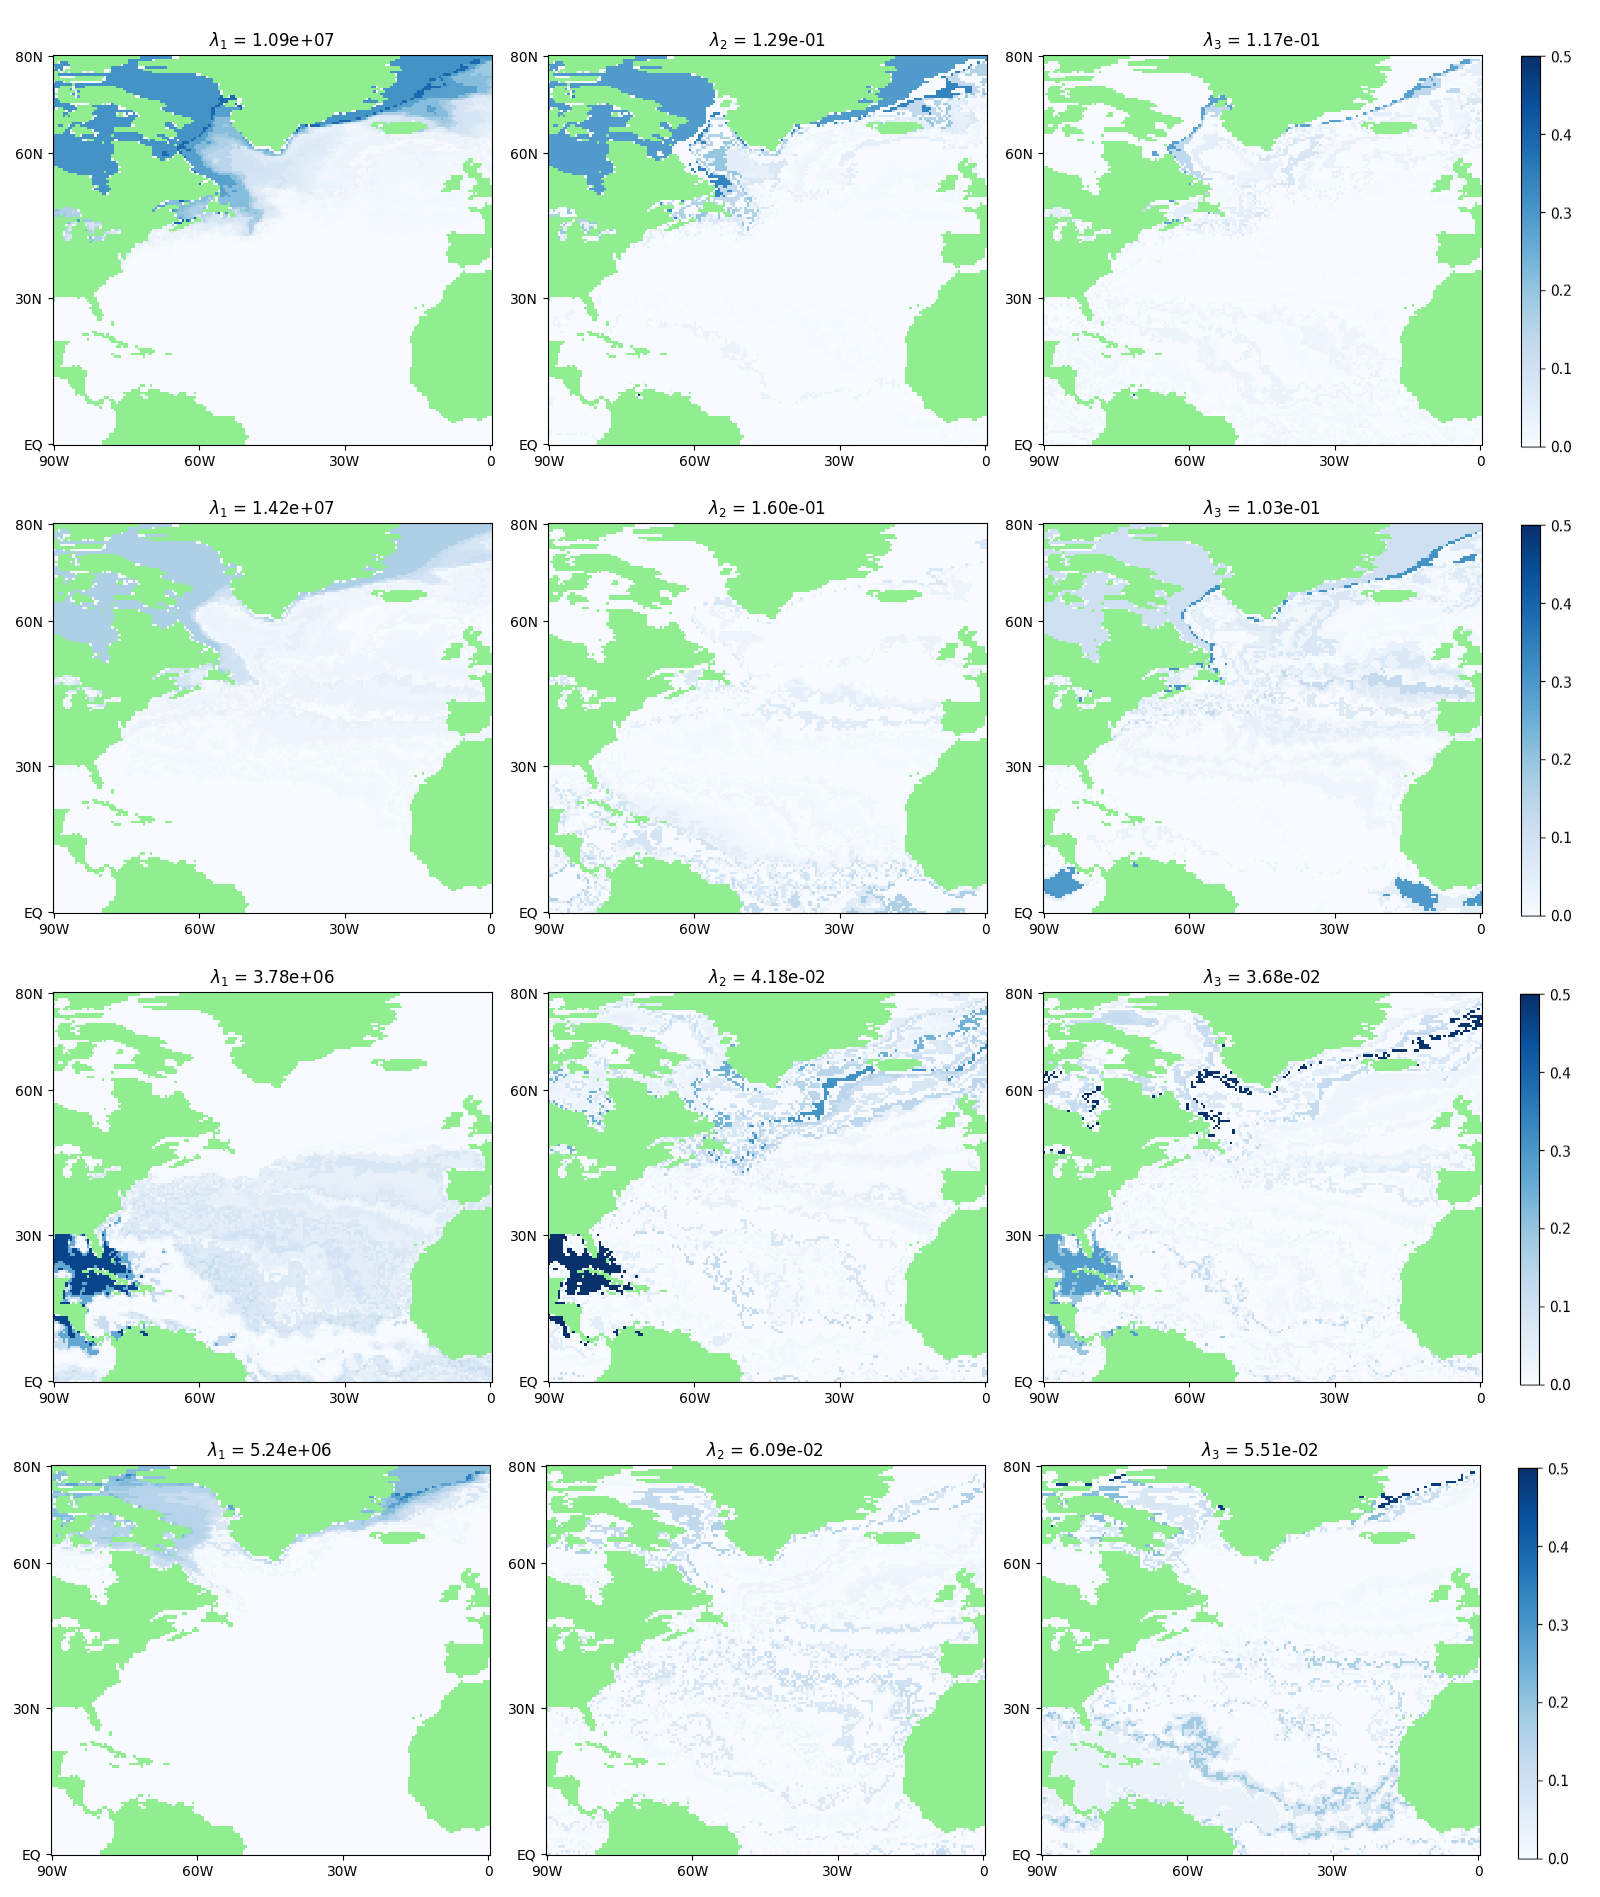
\includegraphics[width=\textwidth]{flux-sst_eigenvectors.png}
	\caption{Первые три собственных вектора из упорядоченного набора для пары Flux-SST за $01.01.23$, $01.04.23$, $01.07.23$ и $01.10.23$}
	\label{fig:Flux-SST_eigenvectors}
\end{figure}

\begin{figure}
	\centering
	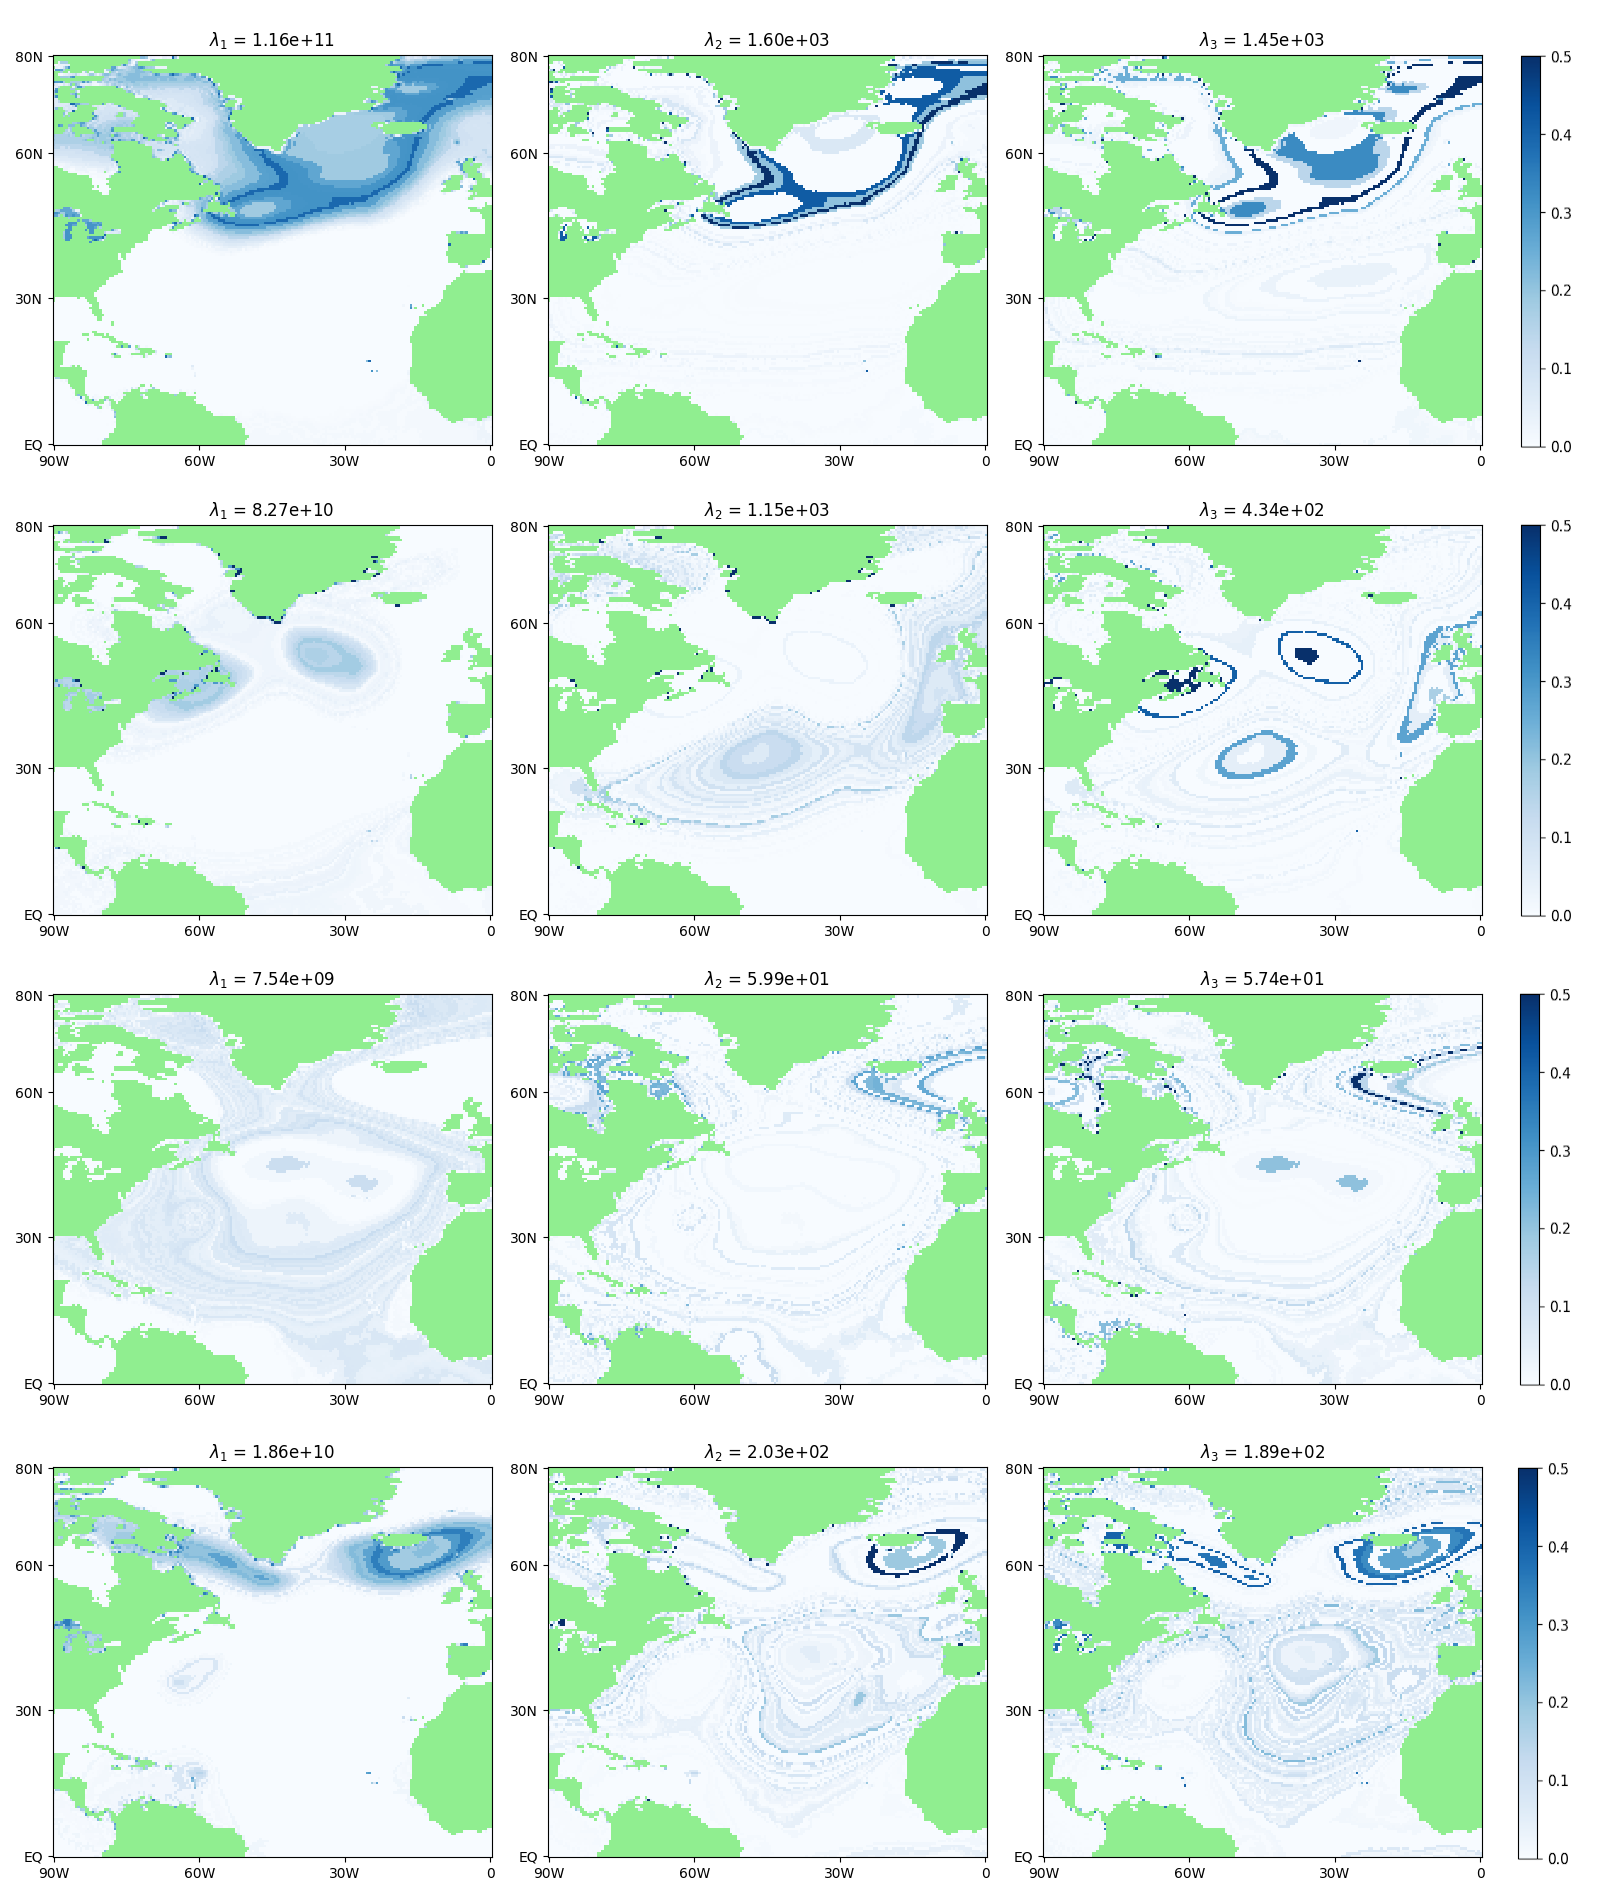
\includegraphics[width=\textwidth]{flux-press_eigenvectors.png}
	\caption{Первые три собственных вектора из упорядоченного набора для пары Flux-Давление за $01.01.23$, $01.04.23$, $01.07.23$ и $01.10.23$}
	\label{fig:Flux-press_eigenvectors}
\end{figure}

\section{Выделение компонент связности для явного и скрытого потоков}
TODO корректура текста
На рис.~\ref{fig:Comps_gulfstqe_dyn}--\ref{fig:Comps_troptqh_diff} верхние графики демонстрируют статистическую структуру процесса теплообмена между океаном и атмосферой в указанных географических точках для двух классов потоков~\cite{perry1977ocean} --  скрытых (далее обозначаются как \verb"qe") и явных (\verb"qh"), -- являющихся составляющими теплового баланса.

Благодаря структурам, возвращаемым функцией \verb"MSMComponents", можно точно отследить, когда те или иные из компонент существовали, прерывались и возобновлялись, и проанализировать их взаимосвязь с реальными физическими процессами. На нижних графиках, содержащих СРС-оценки для динамической и диффузионной компонент, продемонстрирована эволюция весов, то есть вклад соответствующей структурной составляющей в общее развитие процесса во времени.

\begin{figure}[!h]
	\centering
	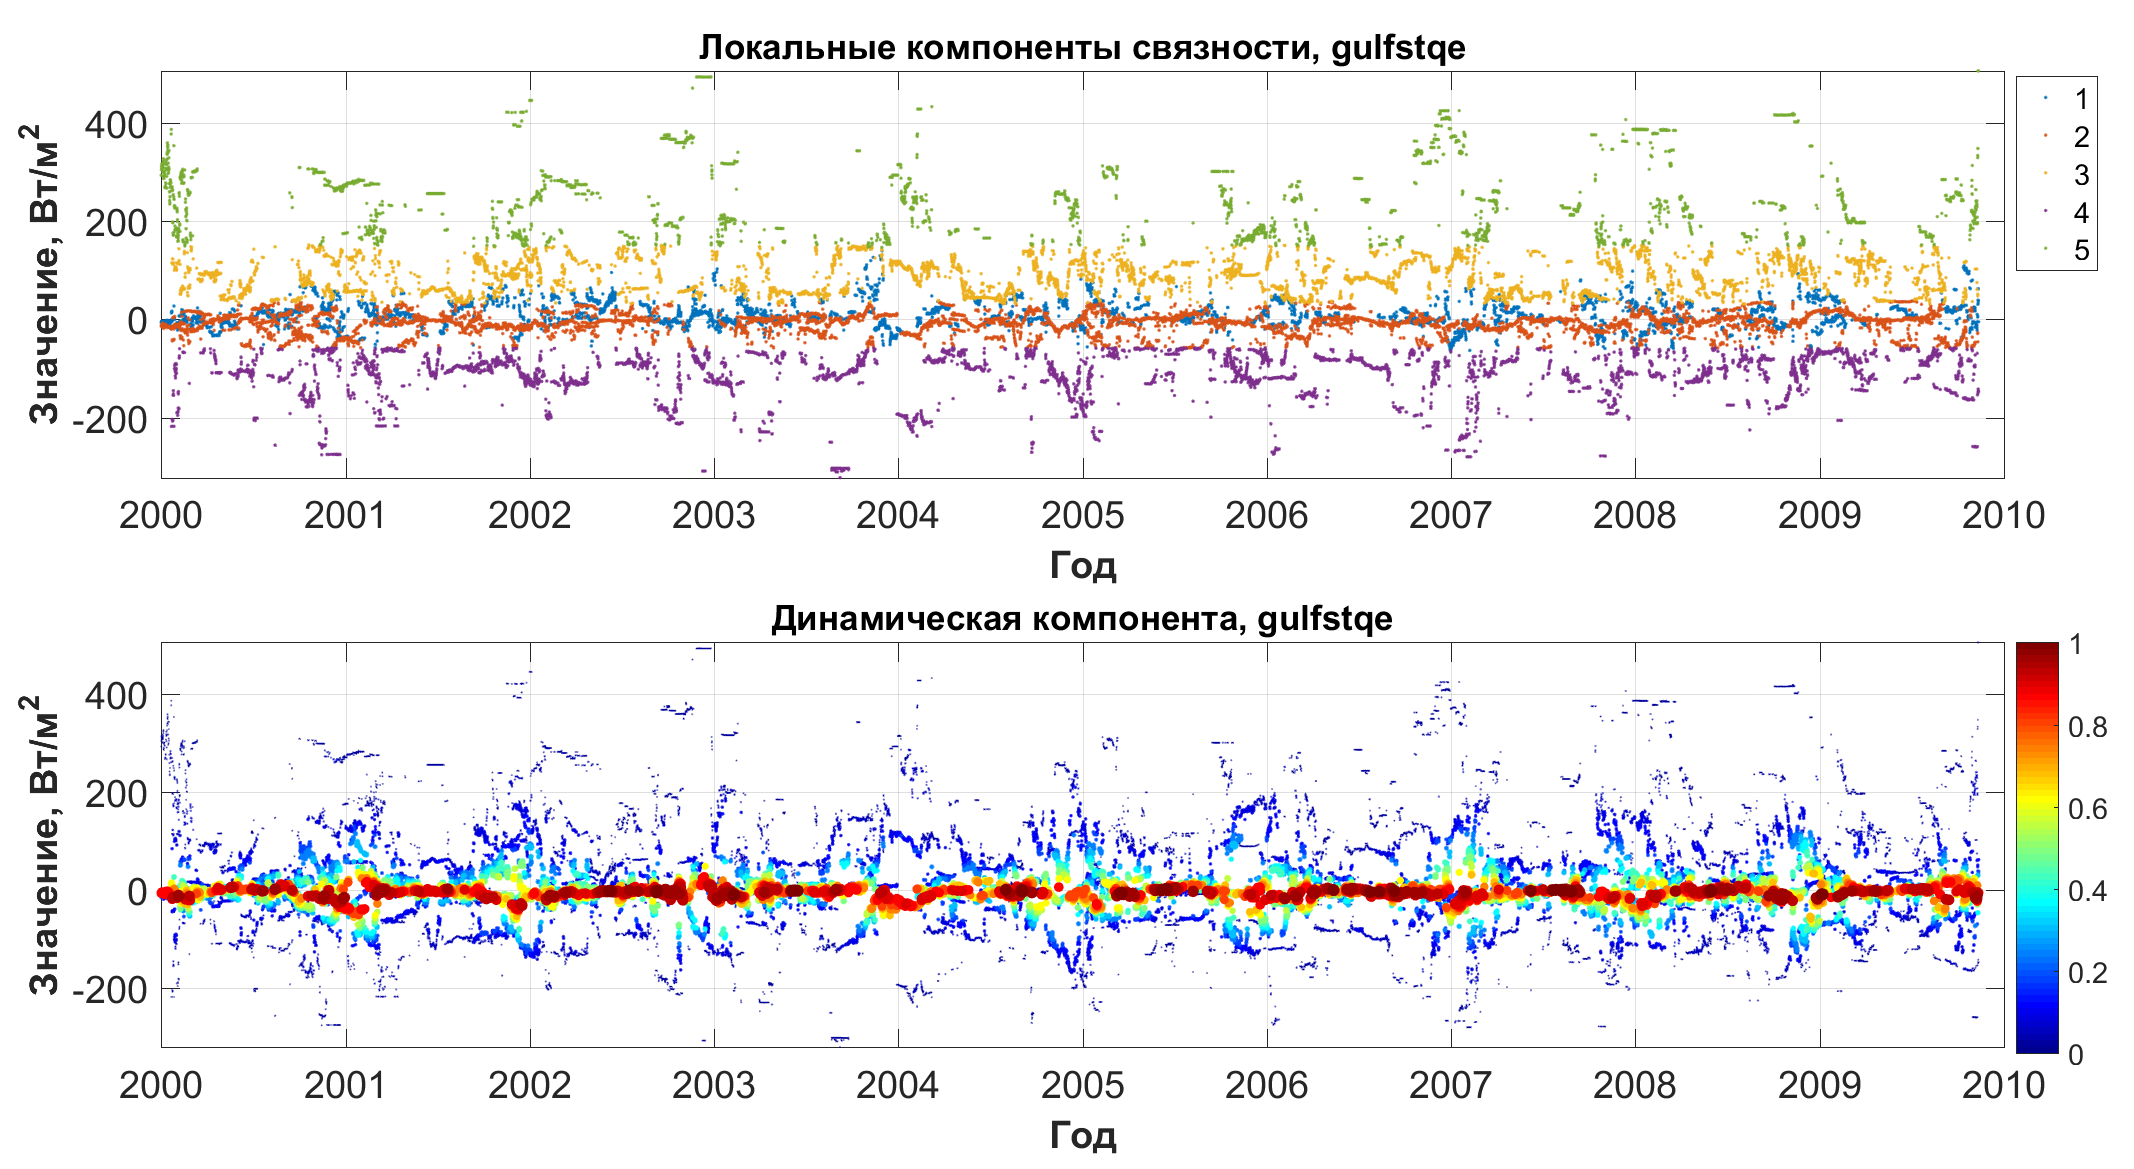
\includegraphics[width=\textwidth,height=0.28\textheight]{Comps_gulfstqe_dyn.png}
	\caption{Оценки распределения сдвига (Гольфстрим, явные потоки)}
	\label{fig:Comps_gulfstqe_dyn}
\end{figure}

\begin{figure}[!h]
	\centering
	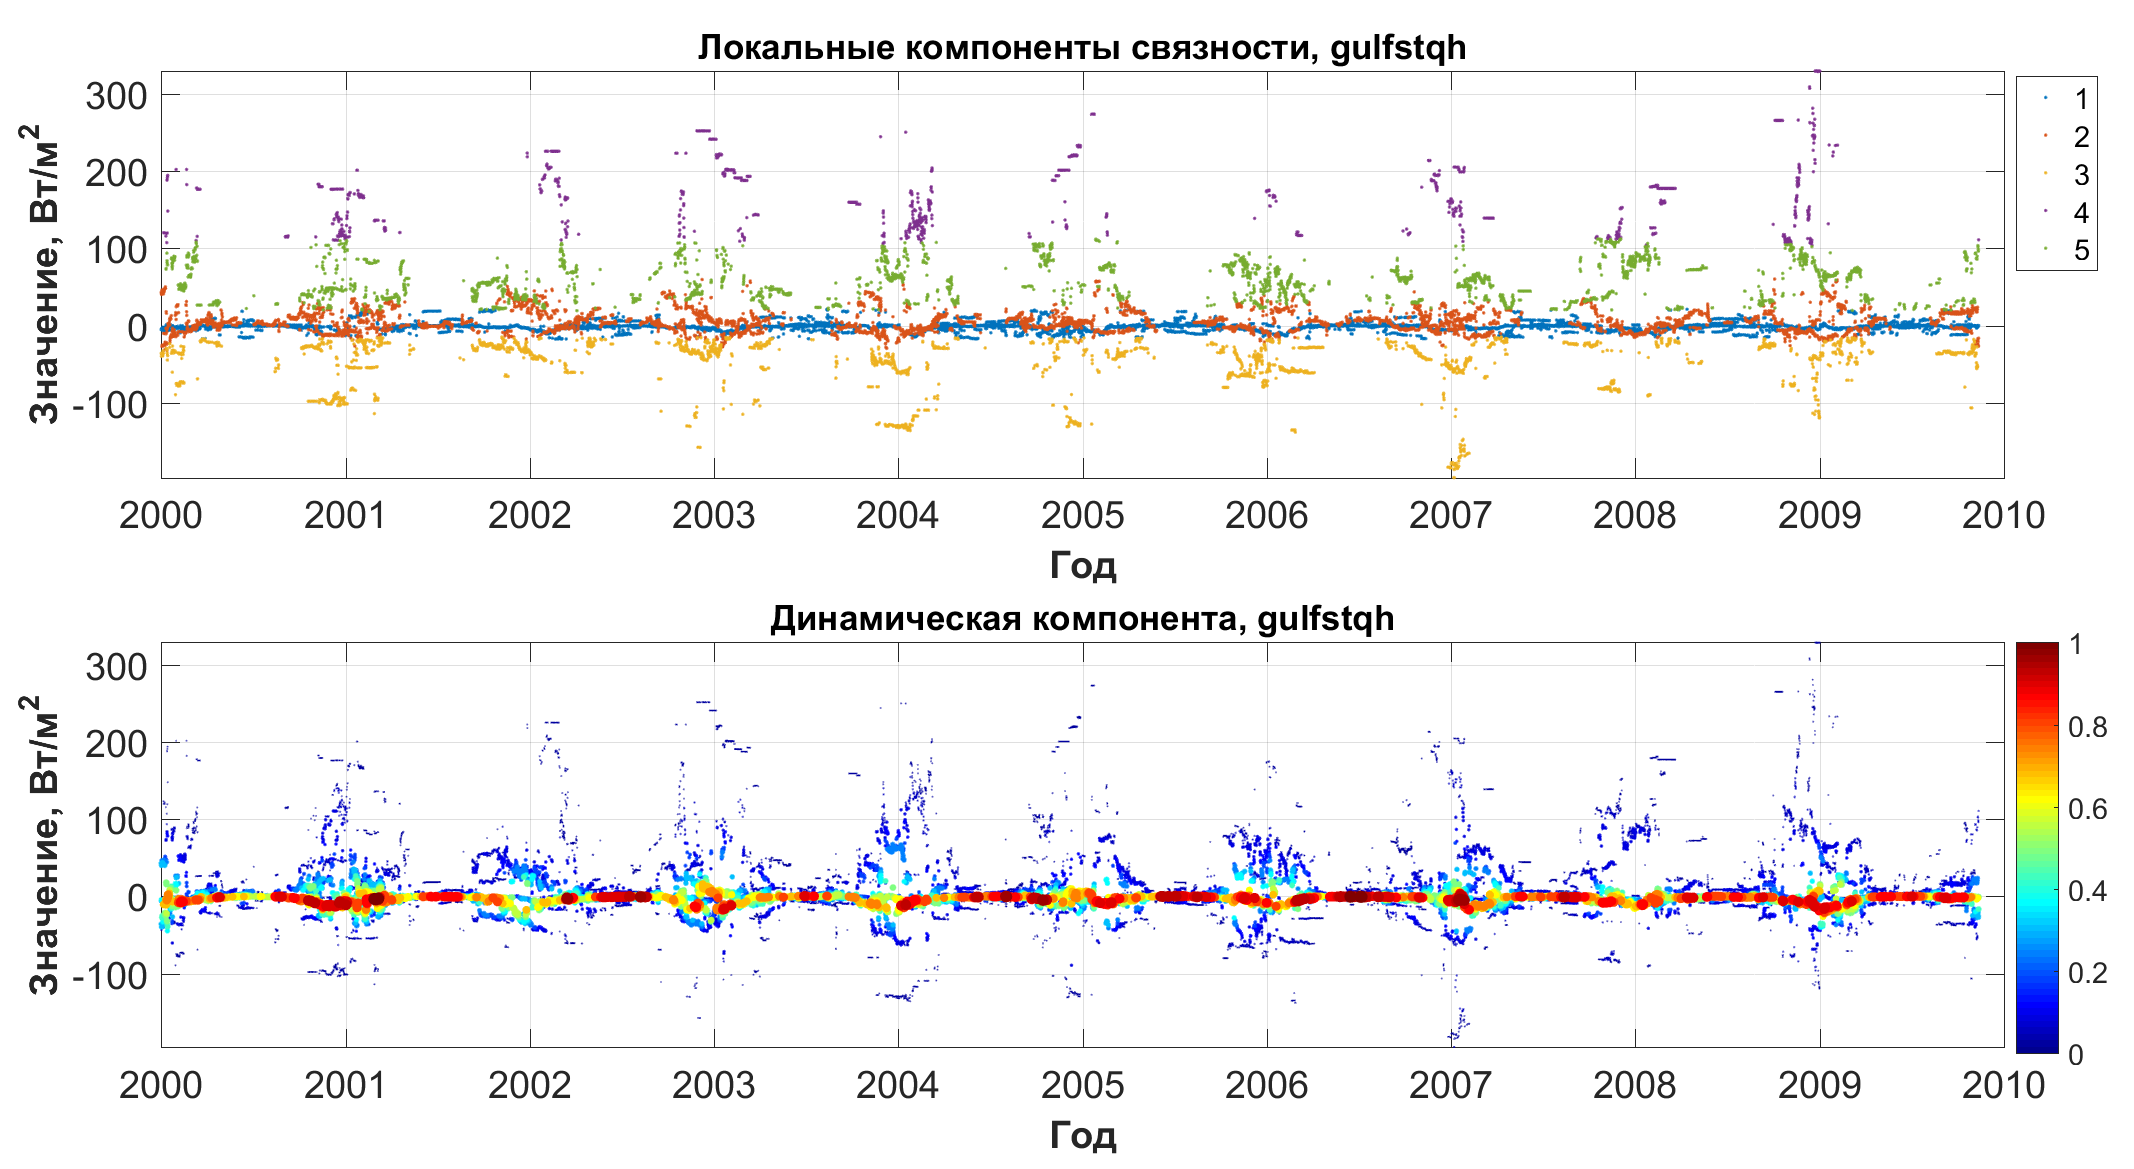
\includegraphics[width=\textwidth,height=0.28\textheight]{Comps_gulfstqh_dyn.png}
	\caption{Оценки распределения сдвига (Гольфстрим, скрытые потоки)}
	\label{fig:Comps_gulfstqh_dyn}
\end{figure}

Для аппроксимации были использованы четырехкомпонентные нормальные смеси, однако при выбранных настройках жадного алгоритма~\ref{AlgGreedy} для всех рядов (за исключением явных потоков в тропиках) были получены пять локальных компонент связности.

\begin{figure}[!h]
	\centering
	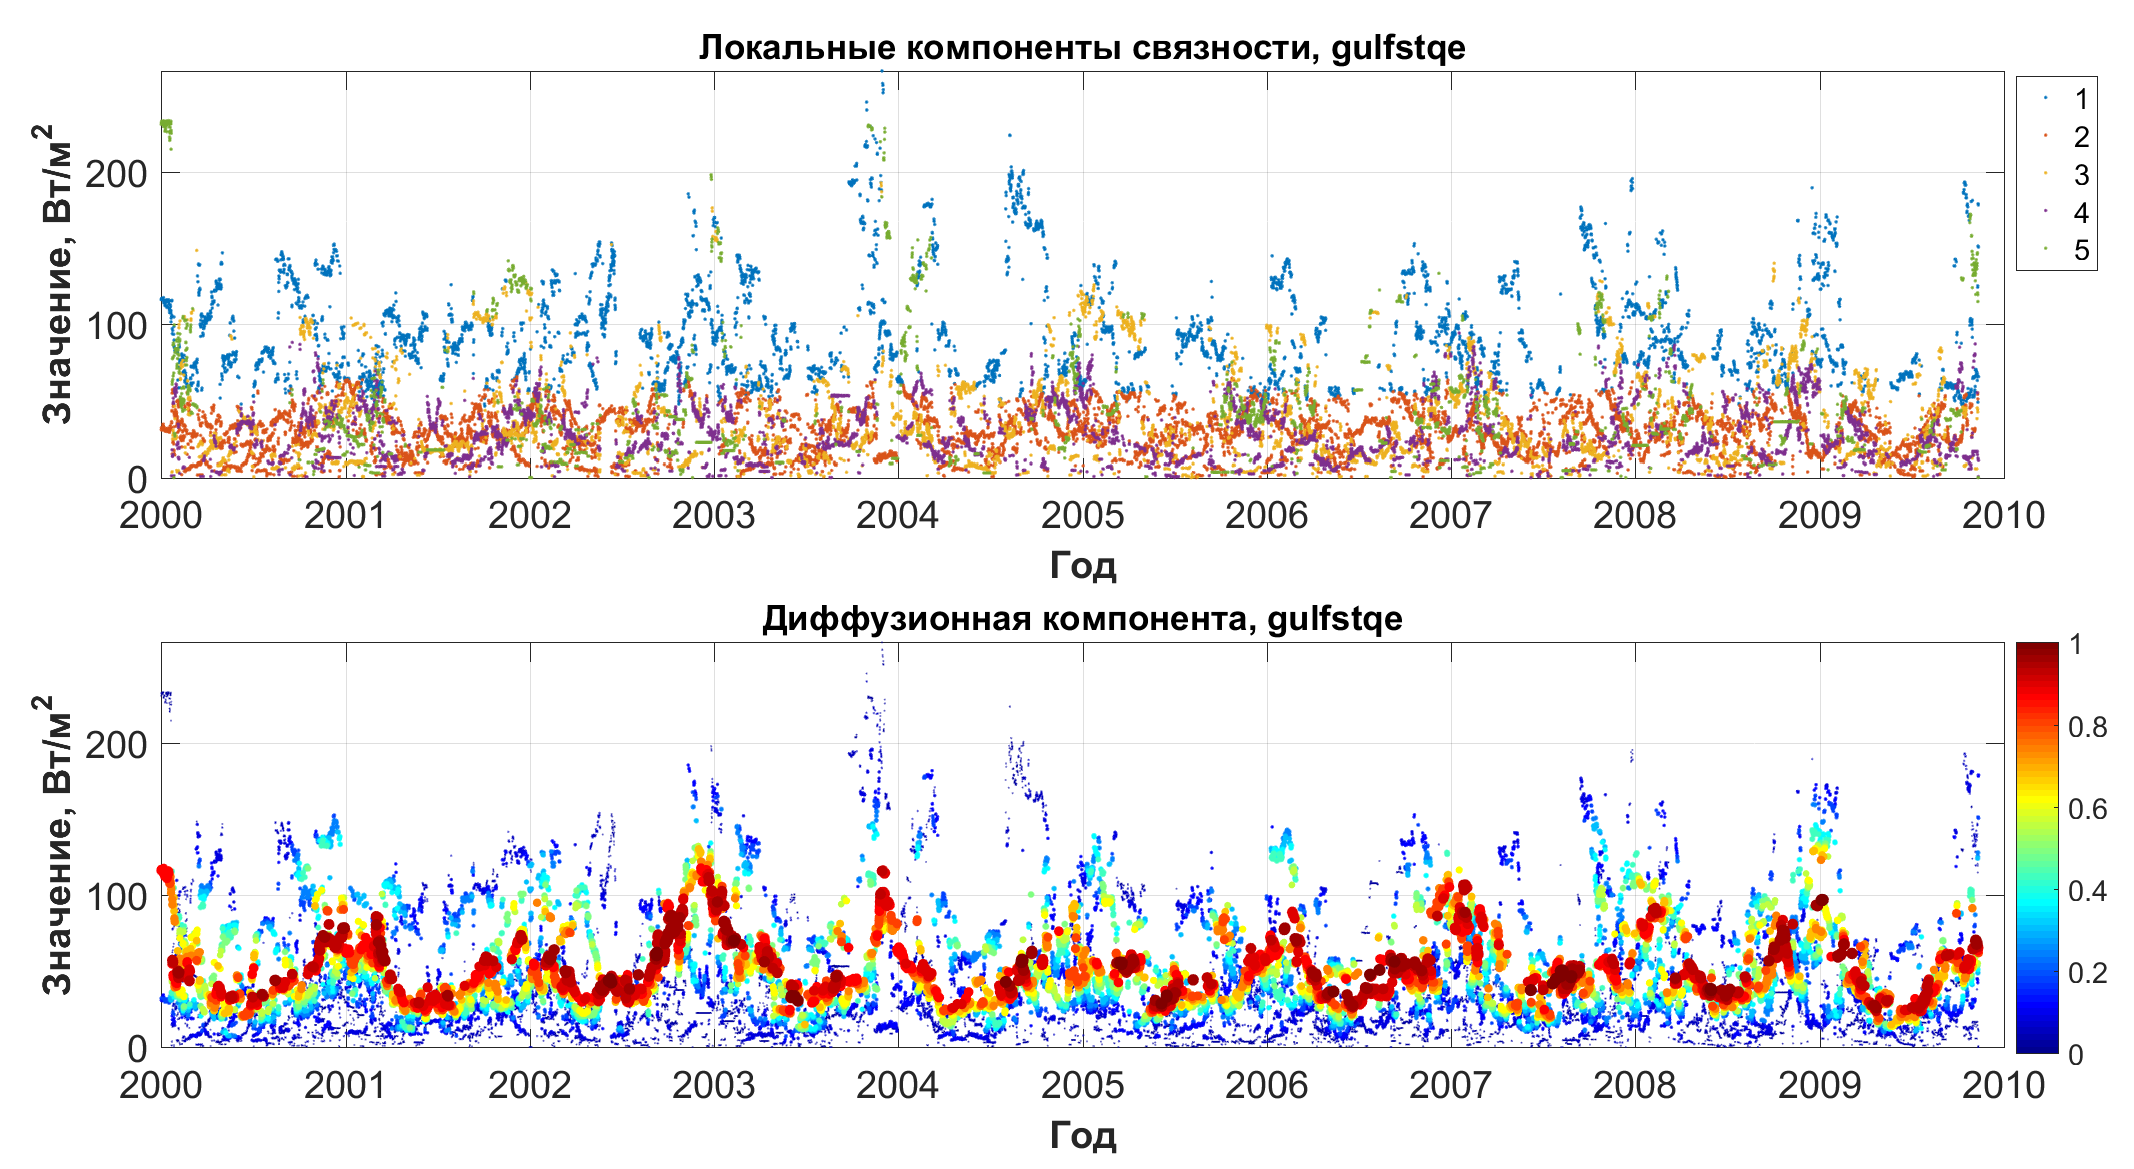
\includegraphics[width=\textwidth,height=0.28\textheight]{Comps_gulfstqe_diff.png}
	\caption{Оценки распределения коэффициента диффузии (Гольфстрим, явные потоки)}
	\label{fig:Comps_gulfstqe_diff}
\end{figure}

\begin{figure}[!h]
	\centering
	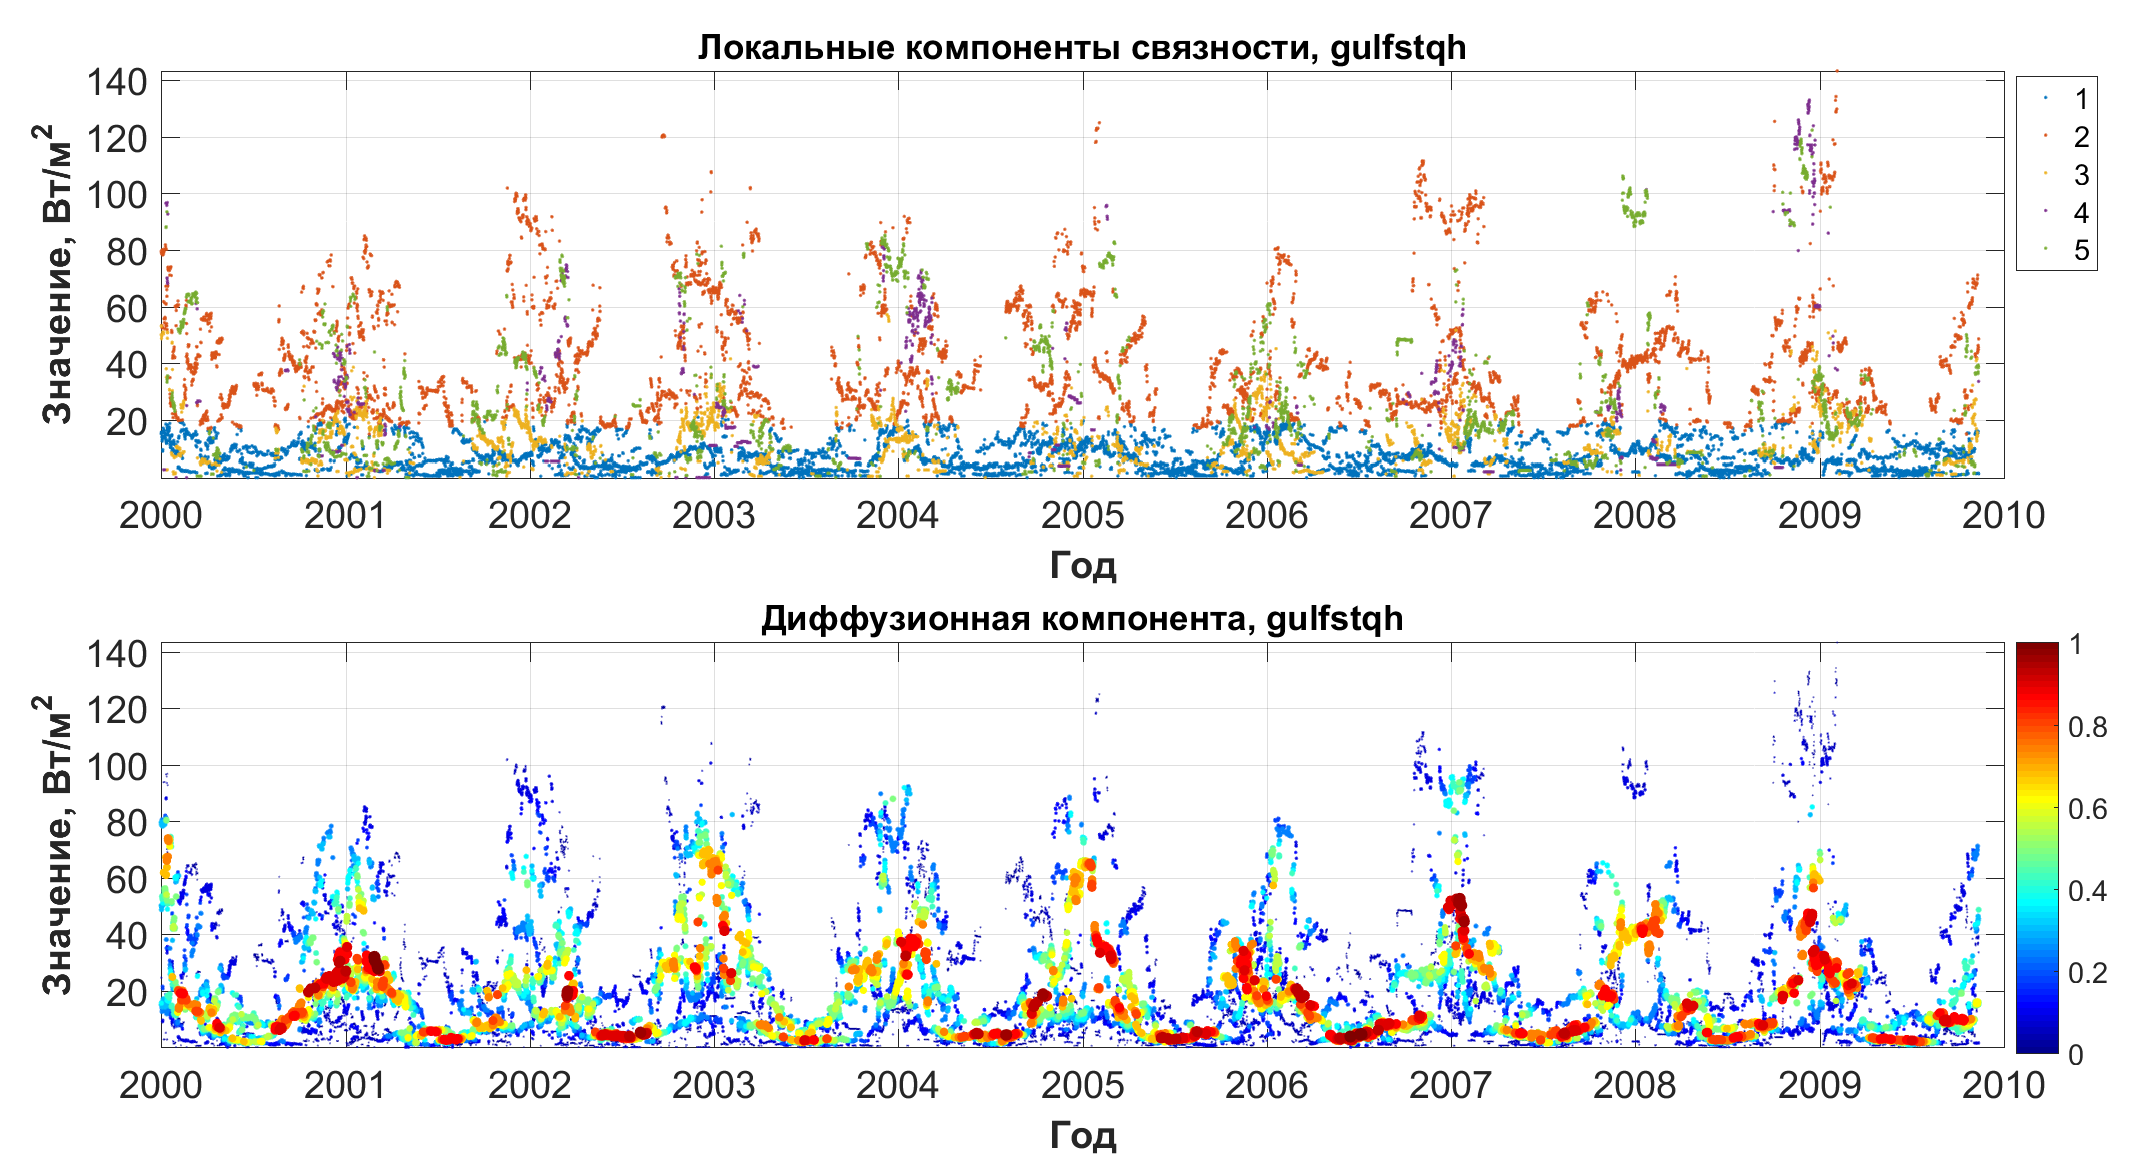
\includegraphics[width=\textwidth,height=0.28\textheight]{Comps_gulfstqh_diff.png}
	\caption{Оценки распределения коэффициента диффузии (Гольфстрим, скрытые потоки)}
	\label{fig:Comps_gulfstqh_diff}
\end{figure}

Видно, что общее число компонент не слишком сильно изменяется, поэтому результаты автоматического определения с помощью жадного алгоритма~\ref{AlgGreedy} варьируются от ряда к ряду не очень существенно. Однако для лучшего учета локальных процессов полученное число компонент ($4$--$5$) может быть расширено за счет повышения чувствительности процедуры путем выбора меньшего порогового значения в формуле~\eqref{Dist}.

\begin{figure}[!h]
	\centering
	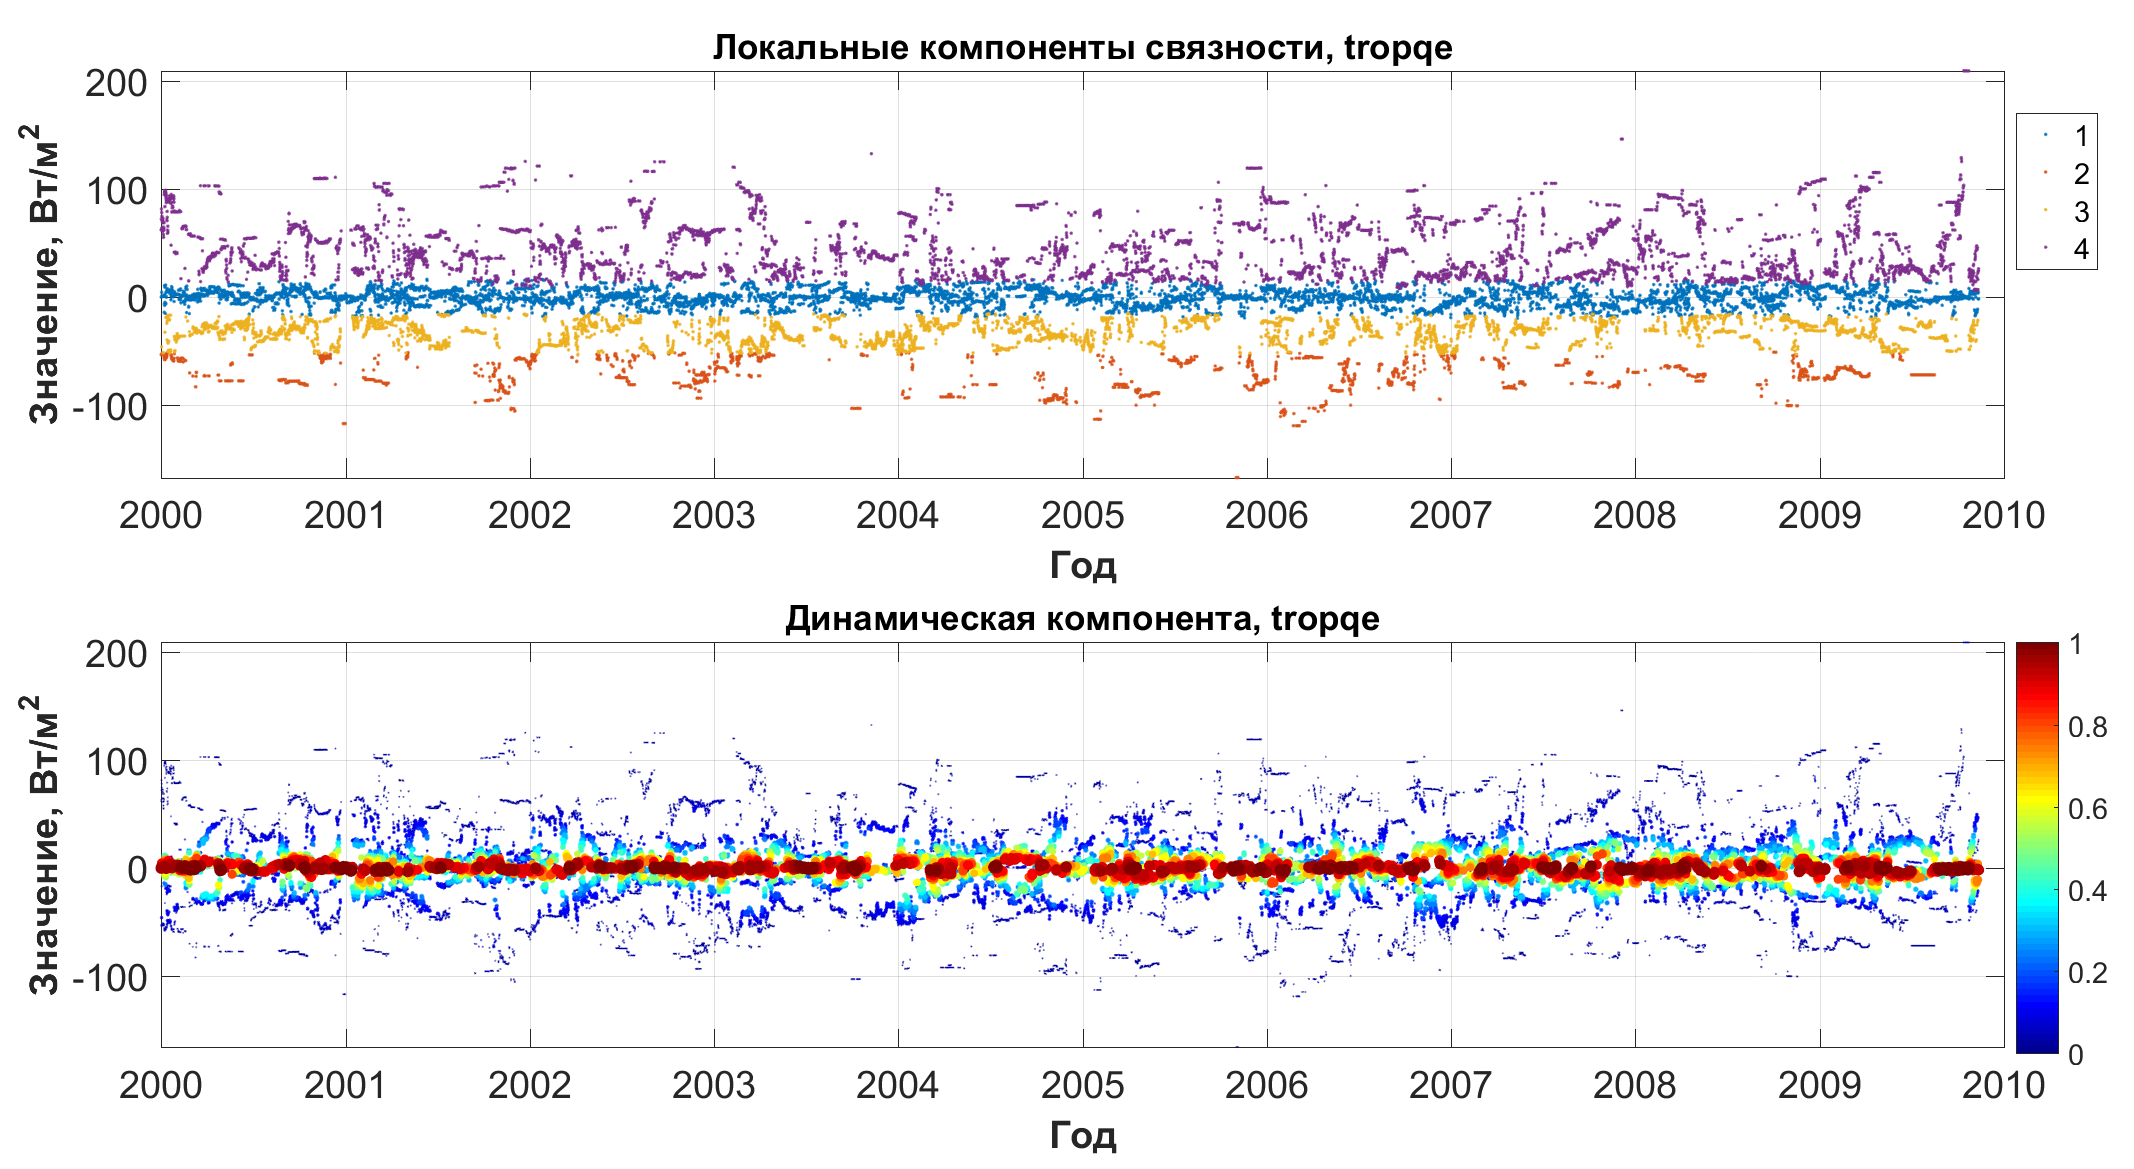
\includegraphics[width=\textwidth,height=0.28\textheight]{Comps_tropqe_dyn.png}
	\caption{Оценки распределения сдвига (тропики, явные потоки)}
	\label{fig:Comps_tropqe_dyn}
\end{figure}

\begin{figure}[!h]
	\centering
	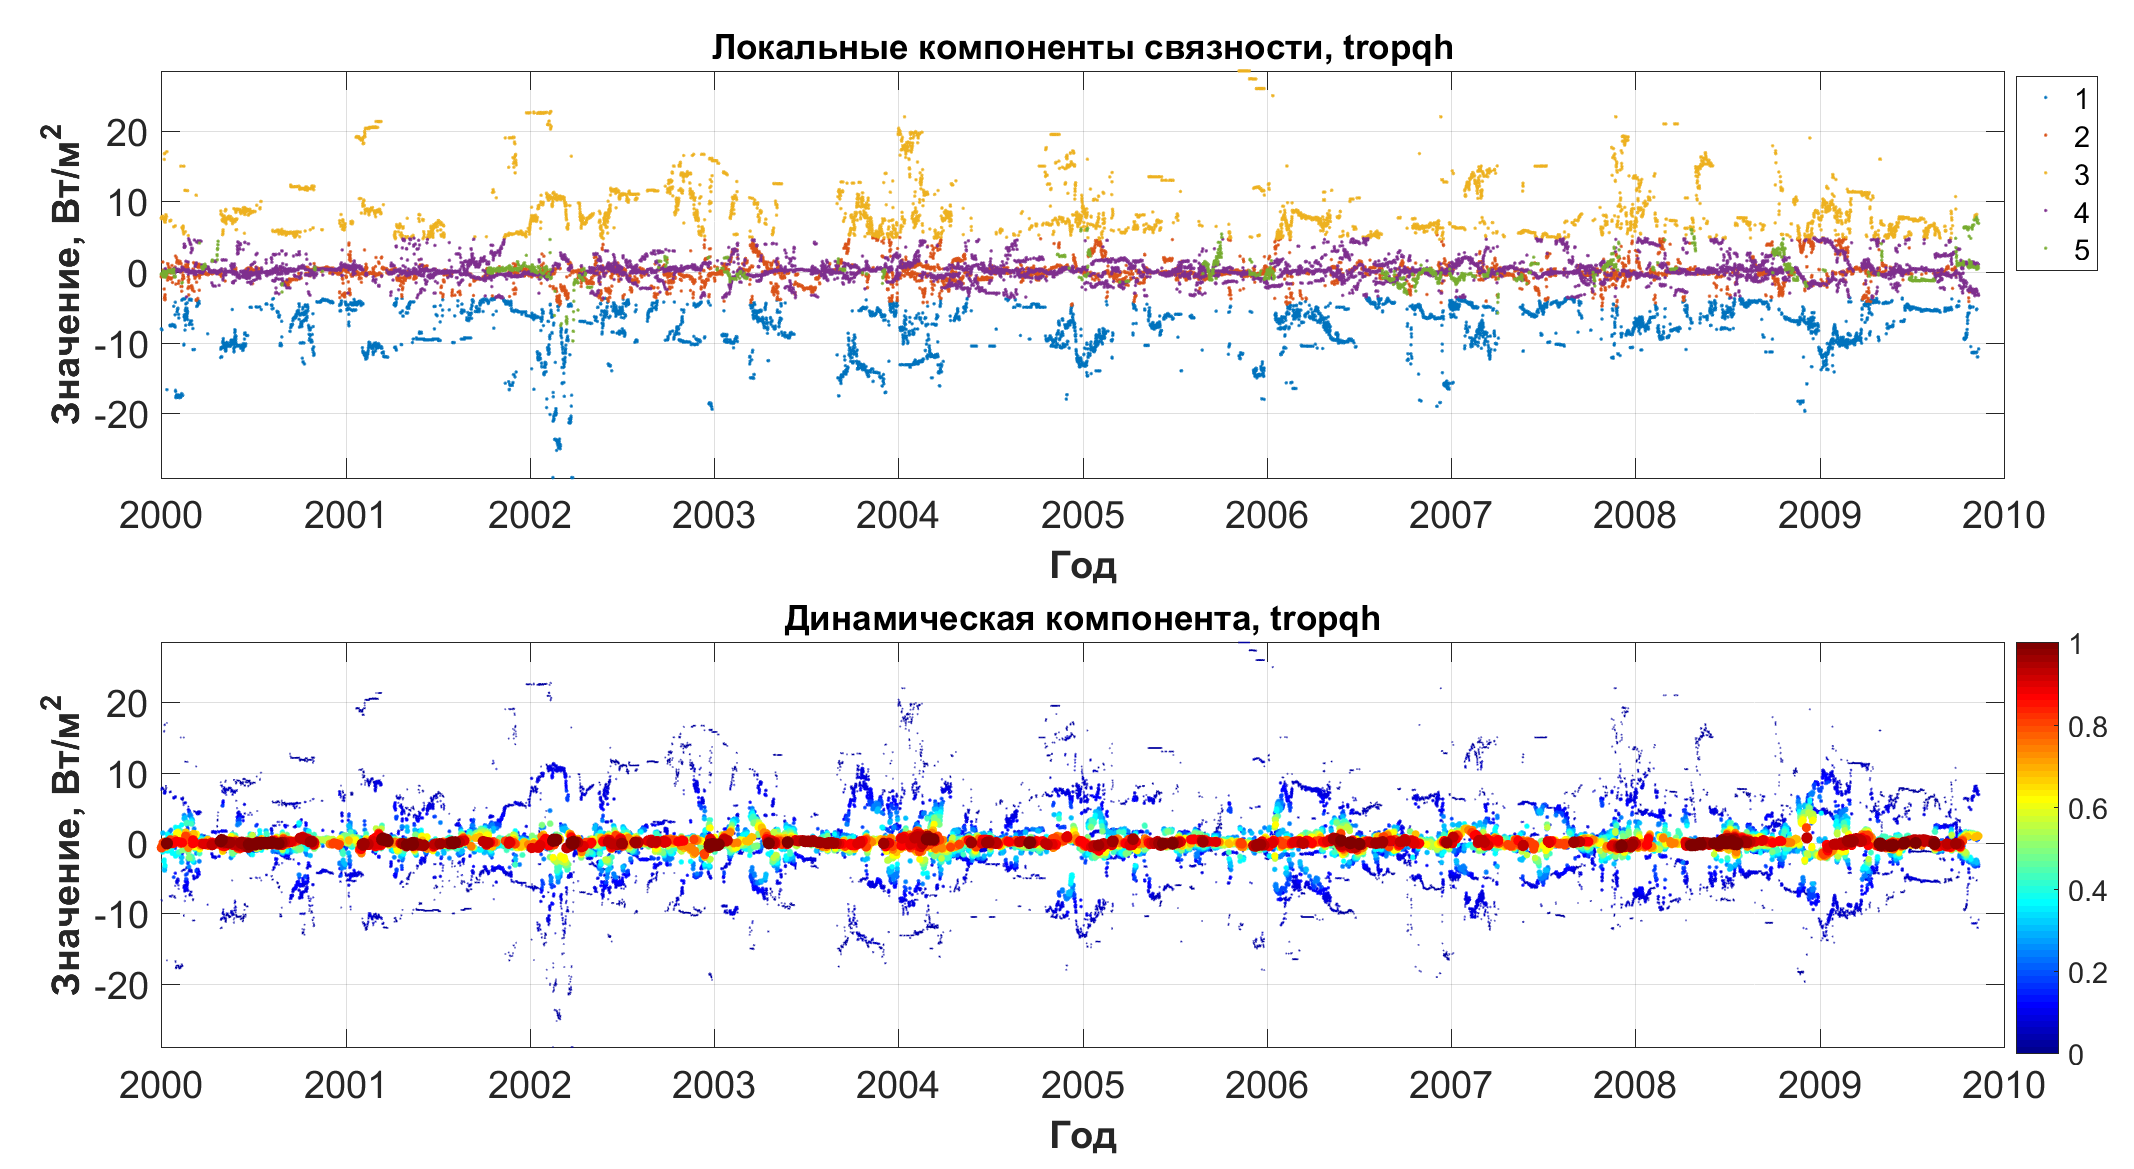
\includegraphics[width=\textwidth,height=0.28\textheight]{Comps_tropqh_dyn.png}
	\caption{Оценки распределения сдвига (тропики, скрытые потоки)}
	\label{fig:Comps_tropqh_dyn}
\end{figure}

\begin{figure}[!h]
	\centering
	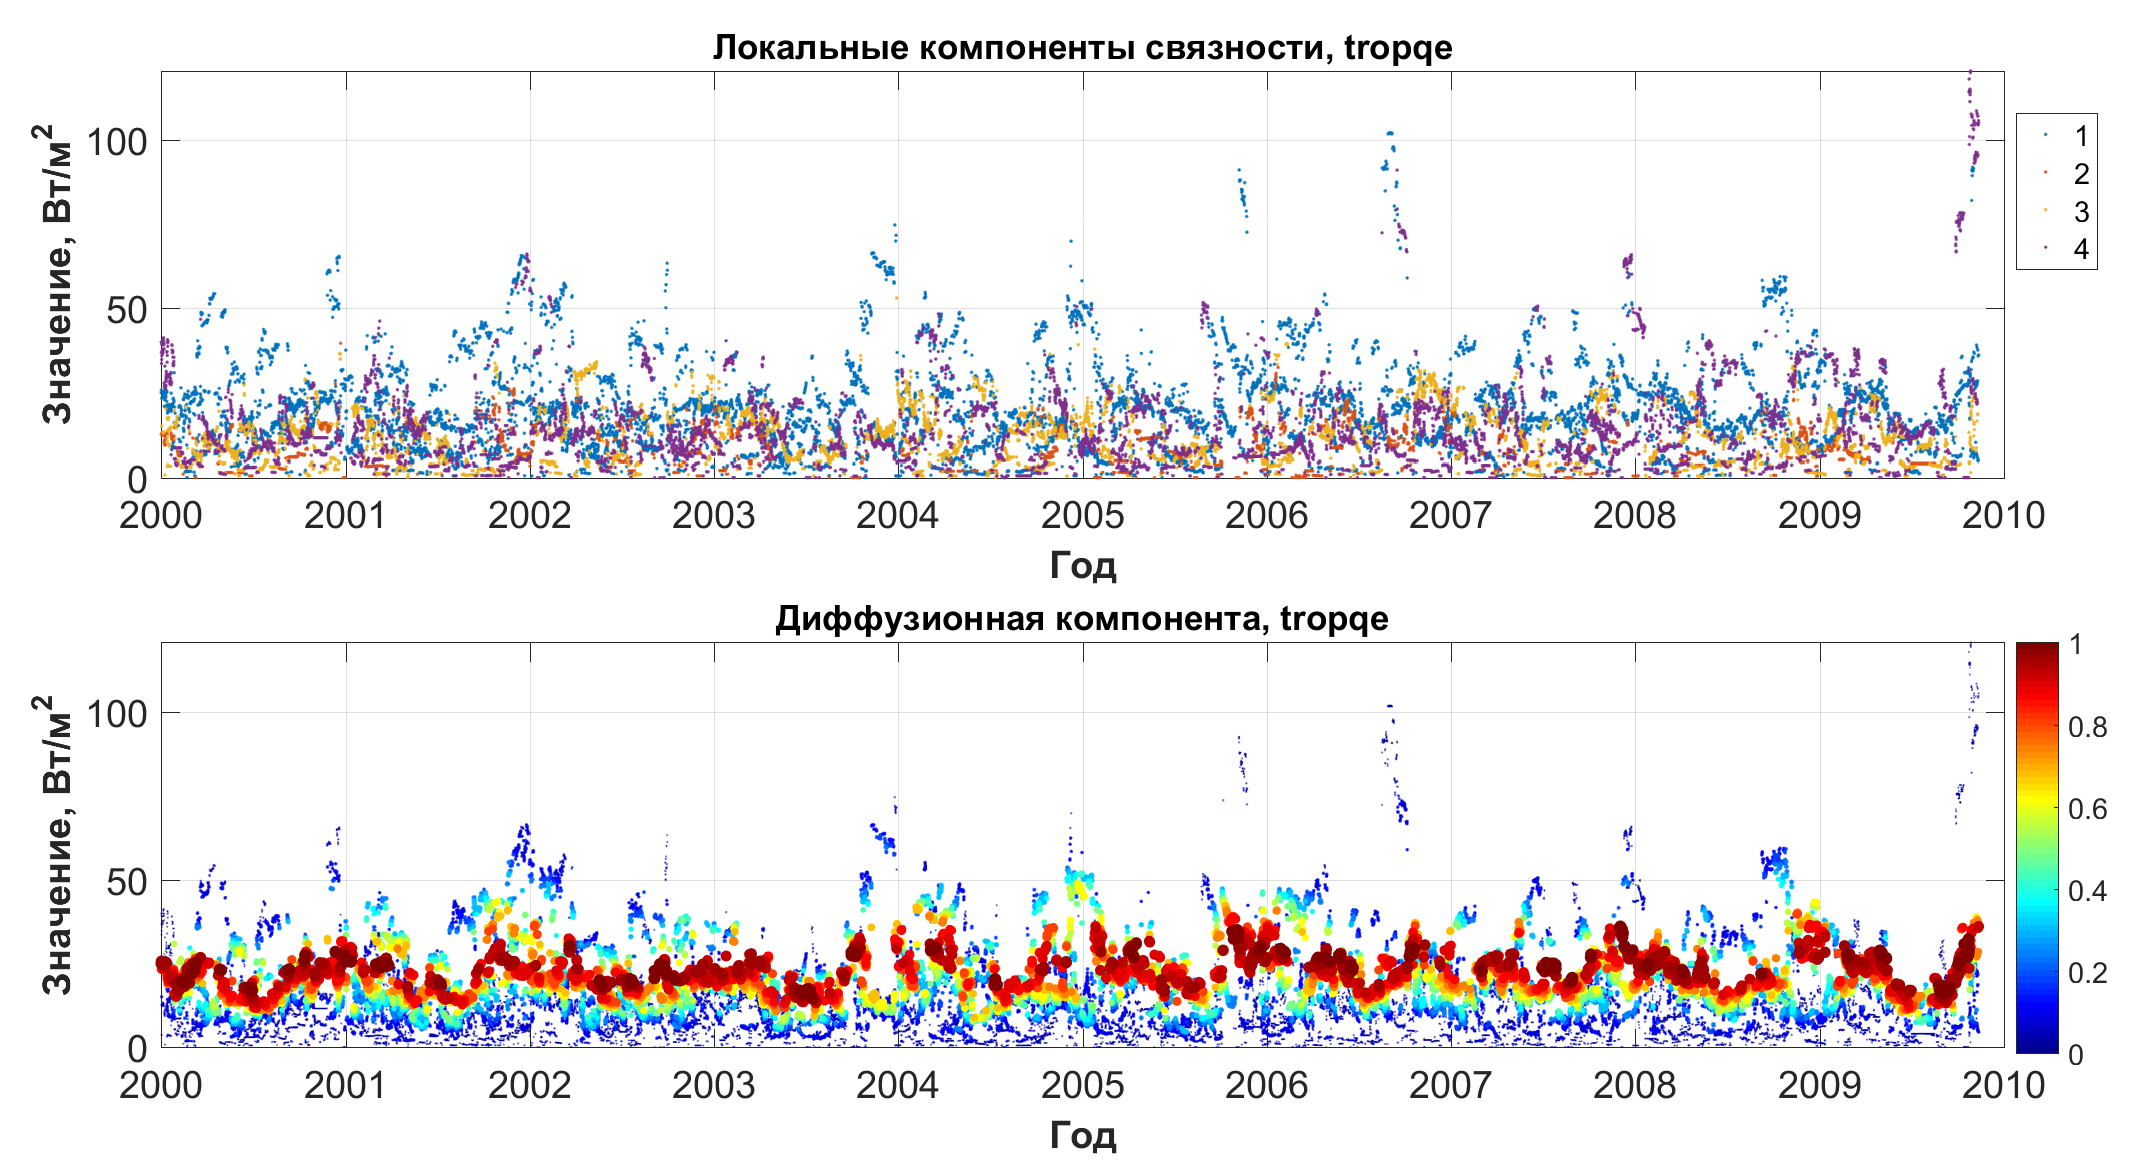
\includegraphics[width=\textwidth,height=0.28\textheight]{Comps_tropqe_diff.png}
	\caption{Оценки распределения коэффициента диффузии (тропики, явные потоки)}
	\label{fig:Comps_troptqe_diff}
\end{figure}

\begin{figure}[!h]
	\centering
	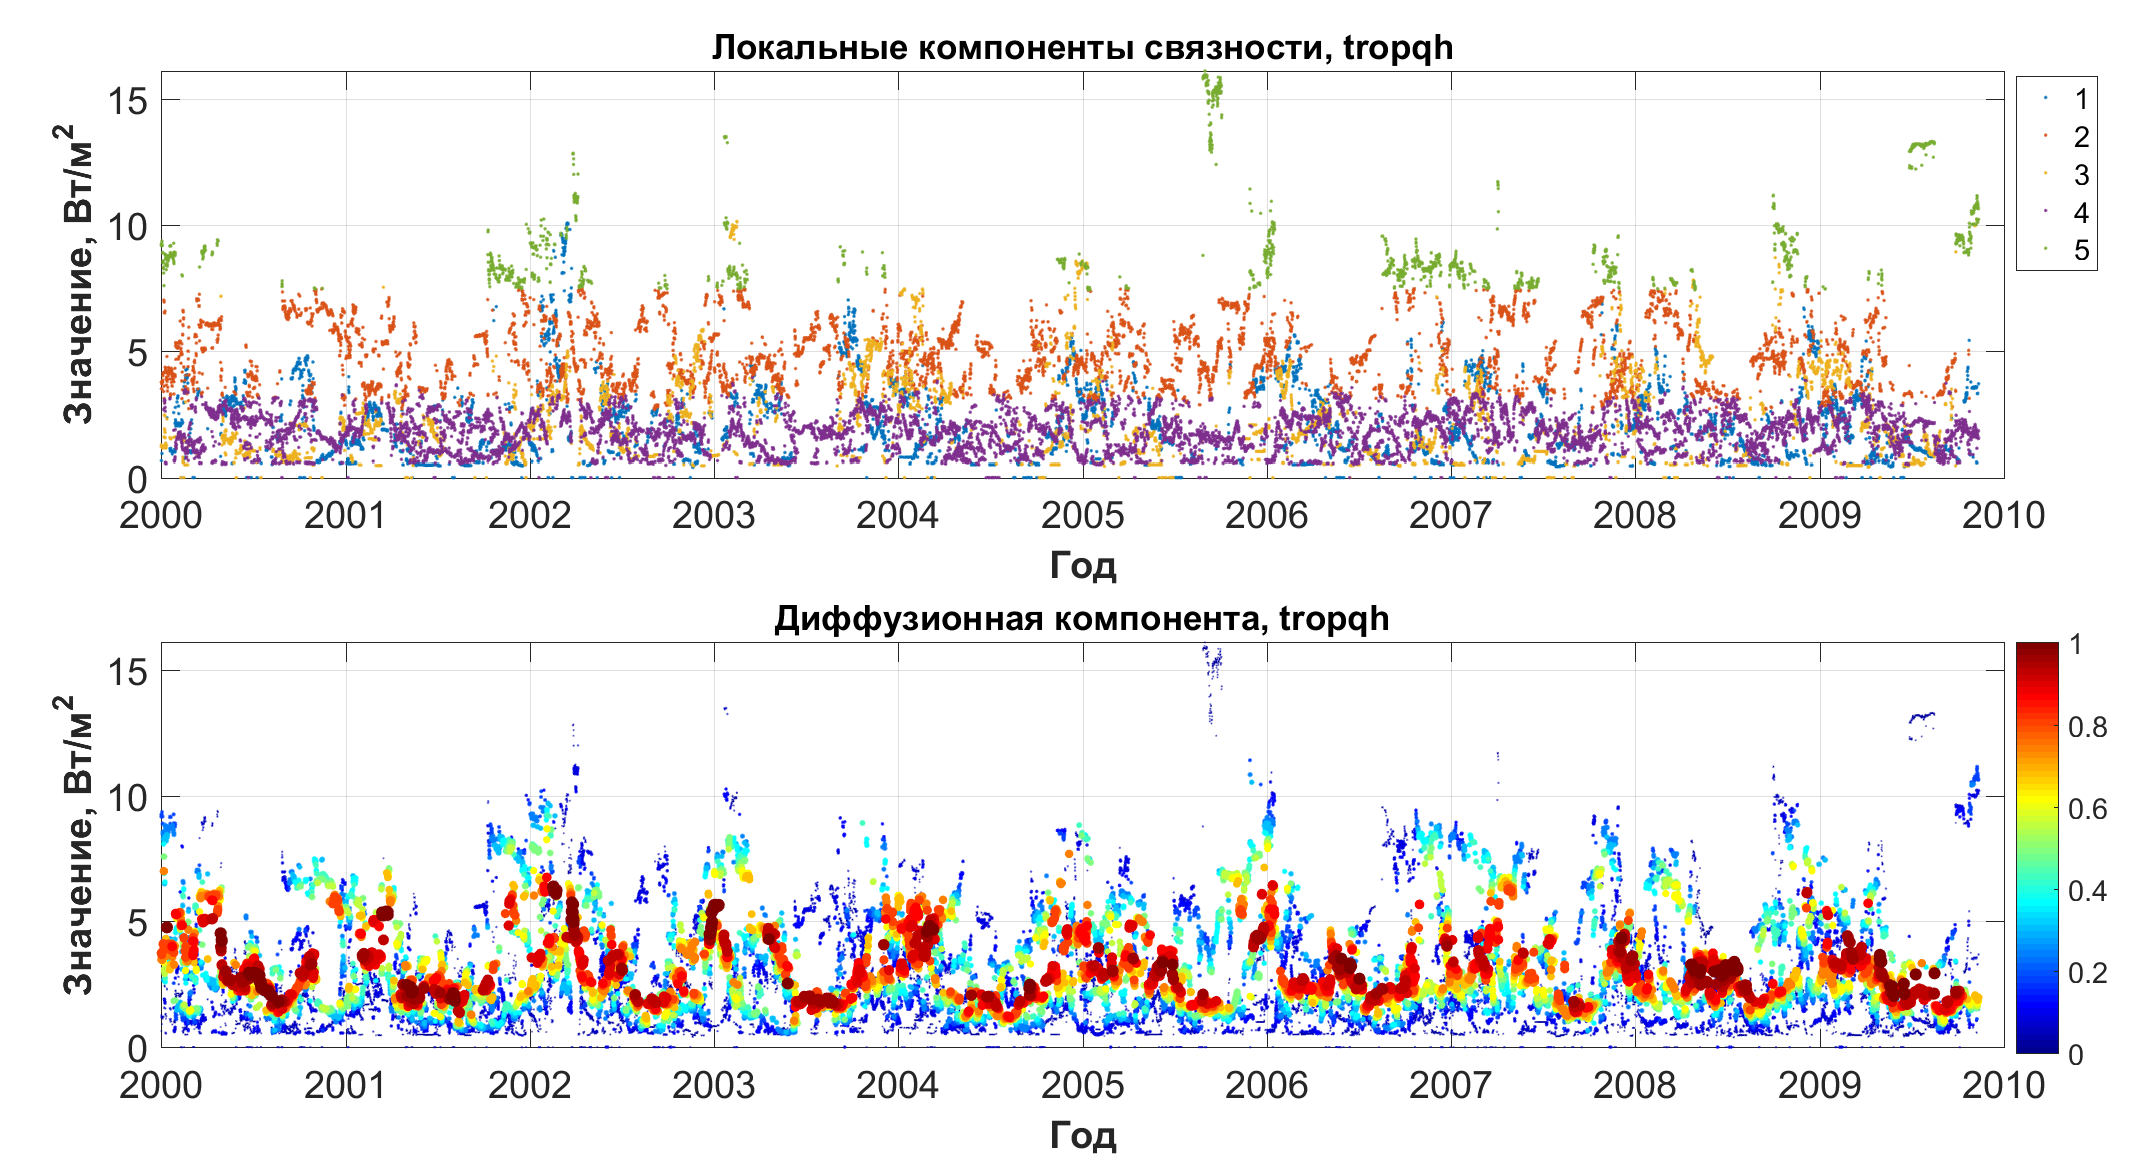
\includegraphics[width=\textwidth,height=0.28\textheight]{Comps_tropqh_diff.png}
	\caption{Оценки распределения коэффициента диффузии (тропики, скрытые потоки)}
	\label{fig:Comps_troptqh_diff}
\end{figure}

В работе описан метод статистического оценивания распределений случайных параметров стохастических дифференциальных уравнений типа Ито с помощью техники скользящего разделения смесей. Предложены дискретные аппроксимации для оценок указанных распределений. С целью изучения изменчивости распределений коэффициентов СДУ во времени предложен алгоритм последовательной идентификации (определения локальной связности) компонент получаемых смесей. В его основу положена комбинация жадного алгоритма для поиска числа компонент и одного из методов кластеризации ($k$- или $c$-средних). Функциональные параметры (компоненты распределения~\eqref{eq:DiffDiscrApprox} как функции времени), полученные в результате описываемых статистических процедур, могут быть использованы при обучении интеллектуальных алгоритмов прогнозирования процессов, удовлетворяющих уравнениям типа~\eqref{eq:Ito}. Применение метода иллюстрируется конкретными примерами анализа процесса теплообмена между атмосферой и океаном.
